\documentclass[8pt]{beamer}
\usepackage[T1]{fontenc}
\usepackage[francais]{babel}
\usepackage{xcolor}
\usepackage{tikz}
\usetikzlibrary{arrows,shapes,tikzmark,fit}
\usepackage{pslatex}
\usepackage{textcomp}
\usepackage[utf8]{inputenc}
\usepackage{wrapfig}
\usepackage{graphicx}
\usepackage[section]{placeins}
\usepackage{lscape}
\usepackage{float}
\usepackage{amssymb}
\usepackage{wasysym}
\usepackage{pgf}
\usepackage{alltt}
\usepackage{eso-pic}
\usepackage{comment}
\usepackage{ulem}
\usepackage{multirow}
\usepackage{makecell}

%\usepackage{colortbl}
%\usepackage{pstricks}

\definecolor{MyGray}{gray}{0.85}
\definecolor{MyGreen}{HTML}{31B404}

\newcommand{\refarticle}[2]{\textit{#1} ~~ \fcolorbox{red}{white}{{\tt #2}}}
\newcommand{\crefarticle}[2]{\begin{center}\textit{#1} ~~ \fcolorbox{red}{white}{{\tt #2}} \end{center}}

\usetheme{Frankfurt}

\graphicspath{{figs/}}

\title[Séminaire 2ieme année]{Développement d'un algorithme de suivi \\ de particules (PFA) pour l'ILC. Outils de surveillance \\ en ligne de qualité de données}
\institute{\normalsize Institut de Physique Nucléaire de Lyon}
\author[R. Eté]{{\large \bf Rémi \'ET\'E} \\ {\bf Directeur de thèse : Imad LAKTINEH}}
\date{8 mars 2017}

\DeclareUnicodeCharacter{00A0}{ }

\setbeamertemplate{itemize items}[ball]
%\addtobeamertemplate{block begin}{\pgfsetfillopacity{0.5}}{\pgfsetfillopacity{1}}

\begin{document}

  %%%%%%%%%%%%%% Page de présentation %%%%%%%%%%%%%%
  \begin{frame}
    \titlepage
    \begin{center}
      
\includegraphics[width=0.2\textwidth]{logo/logo_ipnl.jpg} ~~~
      
\includegraphics[width=0.2\textwidth]{logo/logo-univ-lyon.png} ~~~
      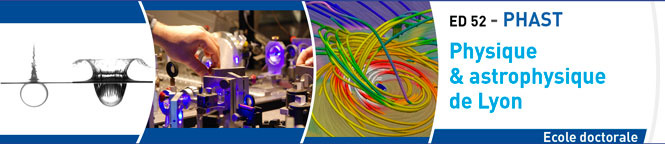
\includegraphics[width=0.5\textwidth]{logo/logo-edphast.jpg}
    \end{center}
  \end{frame}


  \begin{frame}
  \frametitle{Sommaire}
    \tableofcontents
  \end{frame}



  %%%%%%%%%%%%%%%%%%
  %% INTRODUCTION %%
  %%%%%%%%%%%%%%%%%%
  \section{Contexte théorique et expérimental}

  \begin{frame}
  \frametitle{\secname}
    \tableofcontents[currentsection]
  \end{frame}

  \subsection{Le modèle standard}

  %% Modele standard
  \begin{frame}
  \frametitle{\secname}
  \framesubtitle{Le modèle standard}
    \begin{minipage}{0.6\linewidth}
      \begin{block}{Le modèle standard}
        Théorie unifiant 3 des 4 interactions fondamentales :
        \begin{itemize}
          \item L'interaction électromagnétique
          \item L'interaction faible
          \item L'interaction forte
        \end{itemize}
        Théorie de jauge SU(3) $\bigotimes$ SU(2) $\bigotimes$ U(1)
      \end{block}
      ~
    \end{minipage} \hfill
    \begin{minipage}{0.38\linewidth}
      \begin{tikzpicture}
        \node[anchor=south west,inner sep=0] at (0,0) {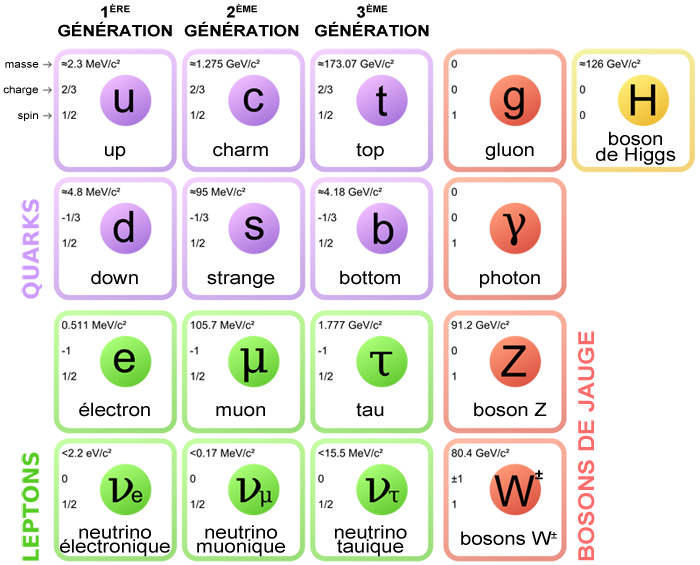
\includegraphics[width=0.9\linewidth]{figs/Particules_elementaires.png}};
        \draw<2>[red, thick, overlay] (3.03,2.1) rectangle (3.65,2.7);
      \end{tikzpicture}
    \end{minipage}
    \begin{minipage}{0.46\linewidth}
      \begin{center}
        \begin{tikzpicture}
          \node[anchor=south west,inner sep=0] at (0,0) {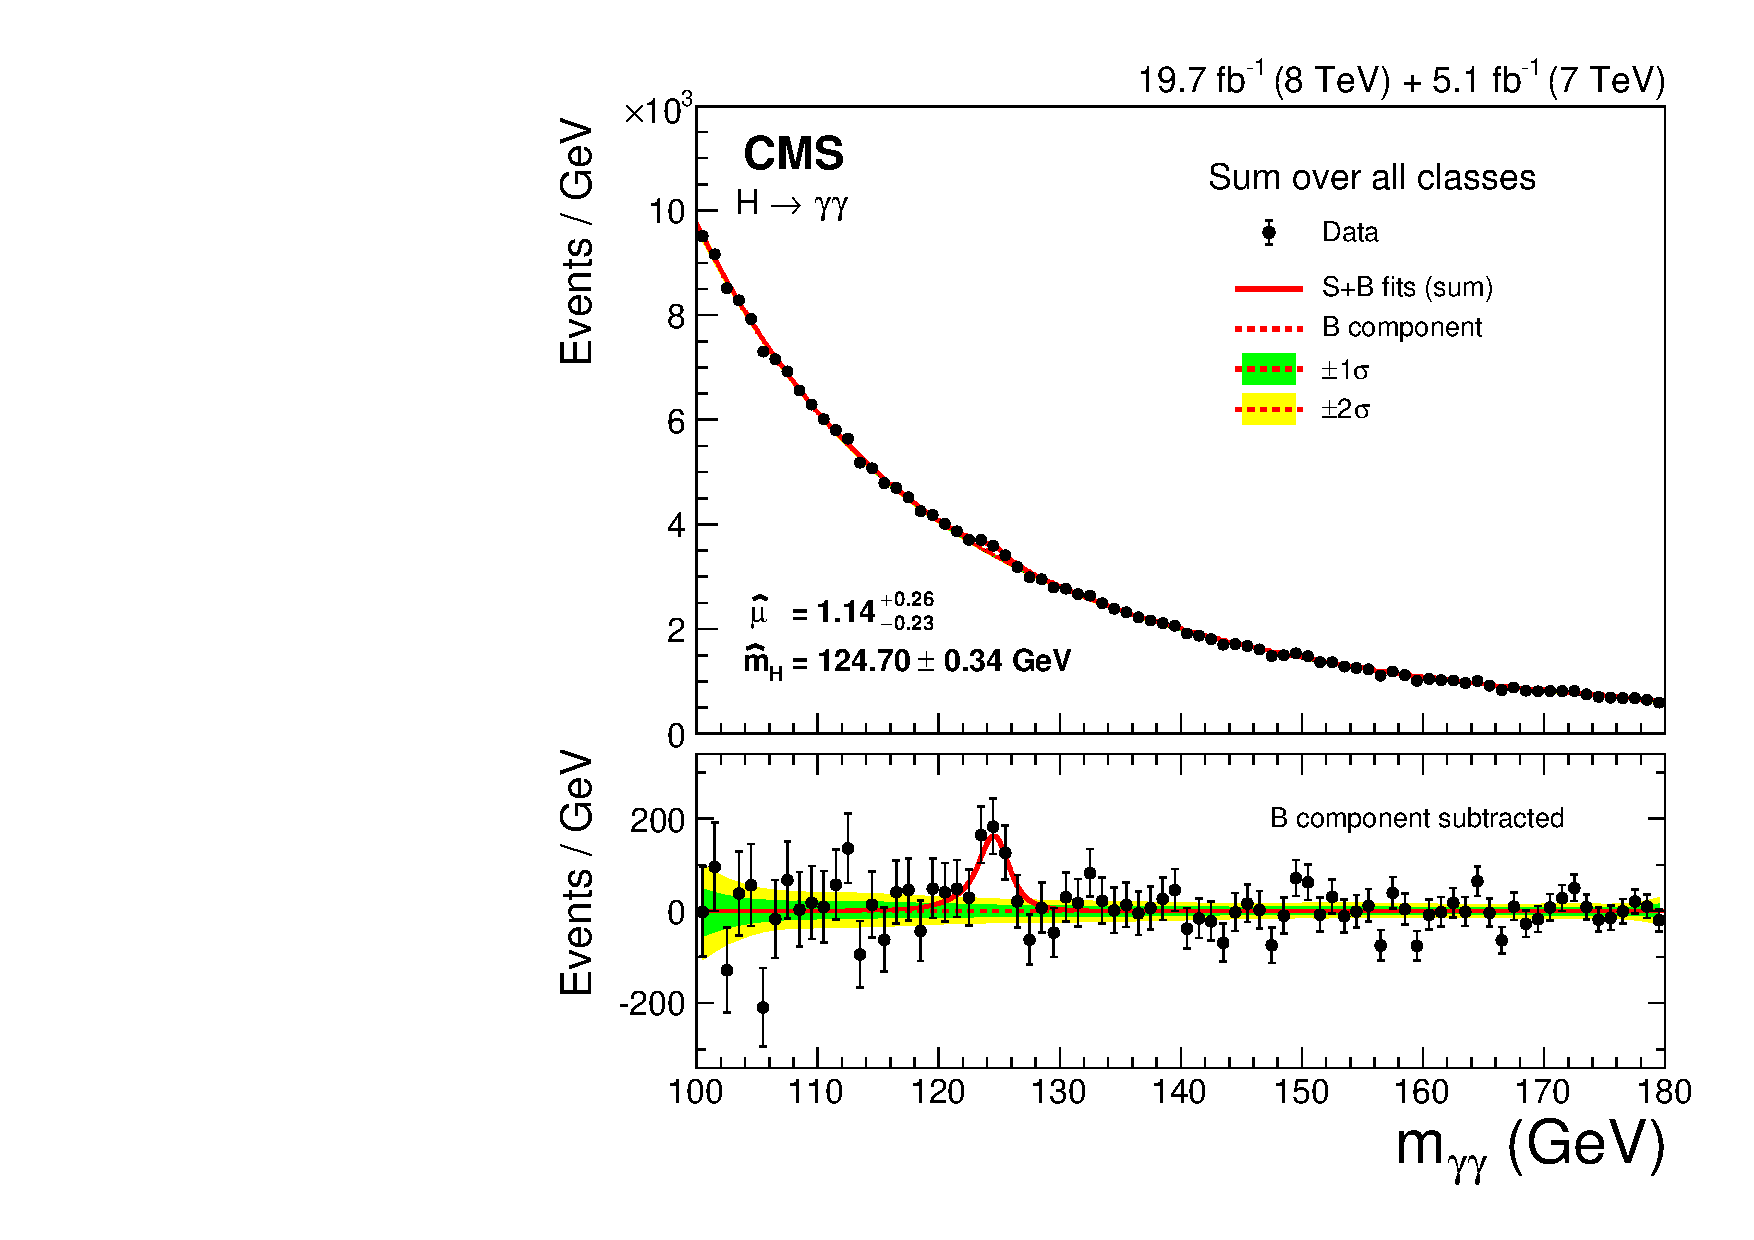
\includegraphics[width=0.8\linewidth]{figs/CMS_Higgs_plot.pdf}};
          \draw<2>[red, thick, overlay] (1.55,1) circle (0.4);
        \end{tikzpicture}
      \end{center}
      \vspace{-0.5cm}
      \crefarticle{CMS-HIG-13-001}{arXiv:1407.0558v2}
    \end{minipage} \hfill
    \begin{minipage}{0.52\linewidth}
      \begin{block}{Des familles et des générations !}
        \begin{itemize}
          \item 12 fermions
          \item 4 bosons de jauge
          \item 1 boson de Higgs
        \end{itemize}
      \end{block}
      \begin{block}{Modèle incomplet}
        \begin{itemize}
          \item Pas de gravitation
          \item Masse/oscillation neutrinos
          \item Asymétrie matière/anti-matière
        \end{itemize}
      \end{block}
    \end{minipage}
    \begin{tikzpicture}
      \draw<2>[red, thick, overlay, ->] (-0.45,4.9) -- (0.3,4.9) -- (0.3,-2.25) -- (-11,-2.25) -- (-11,-0.6) -- (-9.15,-0.6);
    \end{tikzpicture}
  \end{frame}


  \subsection{Le collisionneur linéaire international}

  %% L'ILC
  \begin{frame}
  \frametitle{\secname}
  \framesubtitle{Le collisionneur linéaire international - ILC}
    \begin{center}
      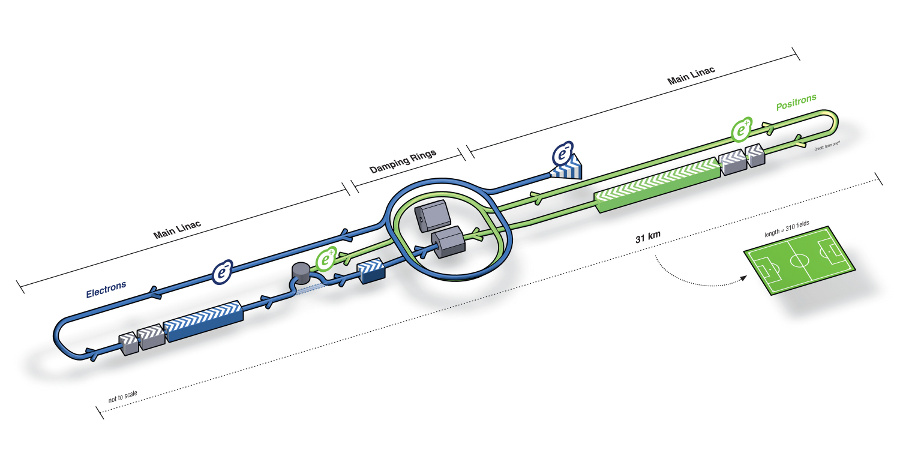
\includegraphics[width=0.55\linewidth]{figs/ilc_layout.jpg}
    \end{center}
    \begin{minipage}{0.51\linewidth}
      \begin{block}{Caractéristiques du collisionneur}
        \begin{itemize}
          \item Collision e$^{+}$ e$^{-}$
          \item Energie : 250-500 GeV (1 TeV ?)
          \item Luminosité : 0.75$\cdot$10$^{34}$-1.8$\cdot$10$^{34}$ cm$^{-2}$s$^{-1}$
          \item Fréquence de collisions : 5 Hz (contre 40 MHz au LHC)
          \item Nb de particules par croisement : 2 $\cdot$ 10$^{10}$
          \item Alimentation pulsée
        \end{itemize}
      \end{block}
    \end{minipage} \hfill
    \begin{minipage}{0.46\linewidth}
      \begin{tikzpicture}
        \node[anchor=south west,inner sep=0] at (0,0) {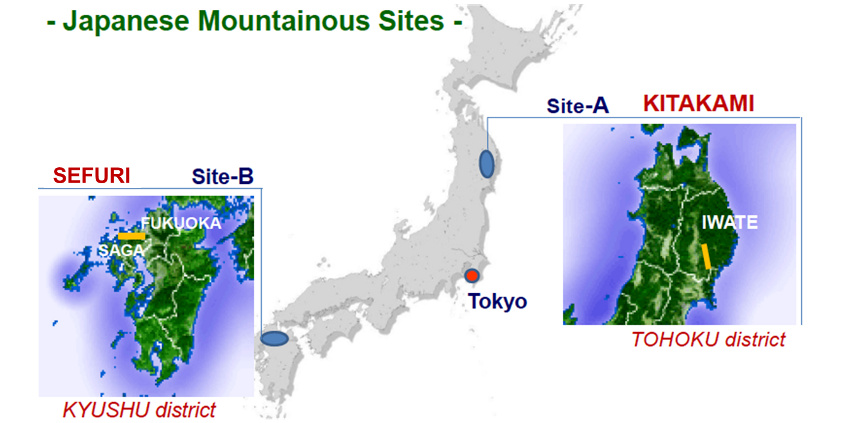
\includegraphics[width=\linewidth]{figs/japanese_sites.jpg}};
        \draw<2>[red, thick, overlay] (3.7,1.3) circle (1.4);
      \end{tikzpicture}
      \crefarticle{ILC Technical Design Report, \\Vol.1 Executive Summary \\}{arXiv:1306.6327}
      % \begin{center}  {\tt } \end{center}
    \end{minipage}
  \end{frame}

  %% Le programme de l'ILC
  \begin{frame}
  \frametitle{\secname}
  \framesubtitle{Le programme physique}
    \begin{center}
      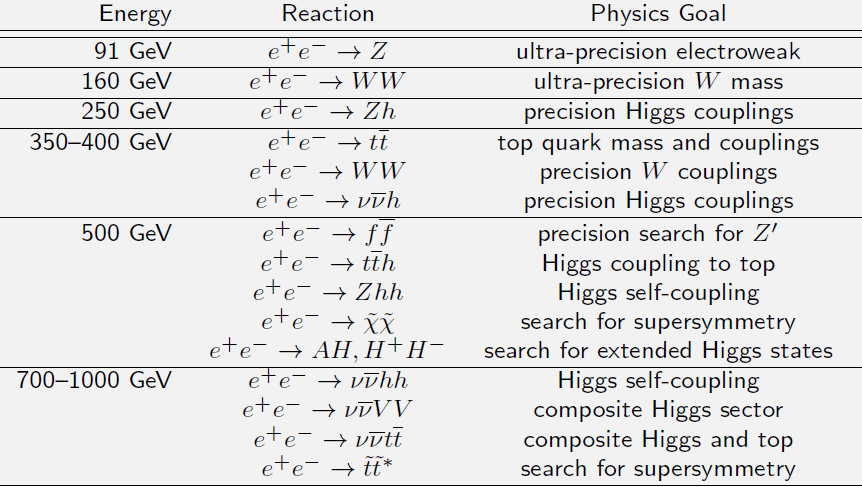
\includegraphics[width=\linewidth]{figs/ilc_program.png}
    \end{center}
    \crefarticle{ILC Technical Design Report, Vol.2 : Physics}{arXiv:1306.6352}
  \end{frame}

  %% ILD et SiD
  \begin{frame}
  \frametitle{\secname}
  \framesubtitle{ILD et SiD}
    \begin{minipage}{0.54\linewidth}
      Deux détecteurs génériques :
      \begin{itemize}
        \item ILD : TPC, plus large, B = 3.5 - 4 T
        \item SiD : Tracker en silicium, plus compact, B = 5 T
      \end{itemize}
      ~ \\
      Installation sur rail coulissant \\
      \crefarticle{ILC Technical Design Report, Vol.4 Detectors \\}{arXiv:1306.6329}
    \end{minipage}
    \begin{minipage}{0.45\linewidth}
      \begin{center}
        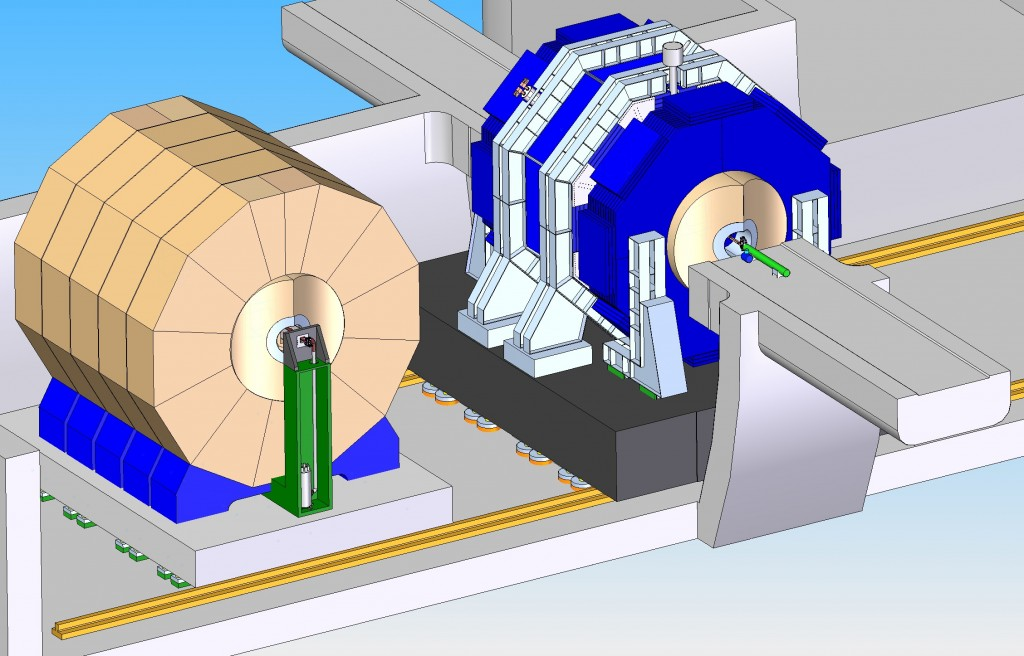
\includegraphics[width=0.94\linewidth]{figs/ild_sid.jpg}
      \end{center}
    \end{minipage}
    ~ \\
    ~ \\
    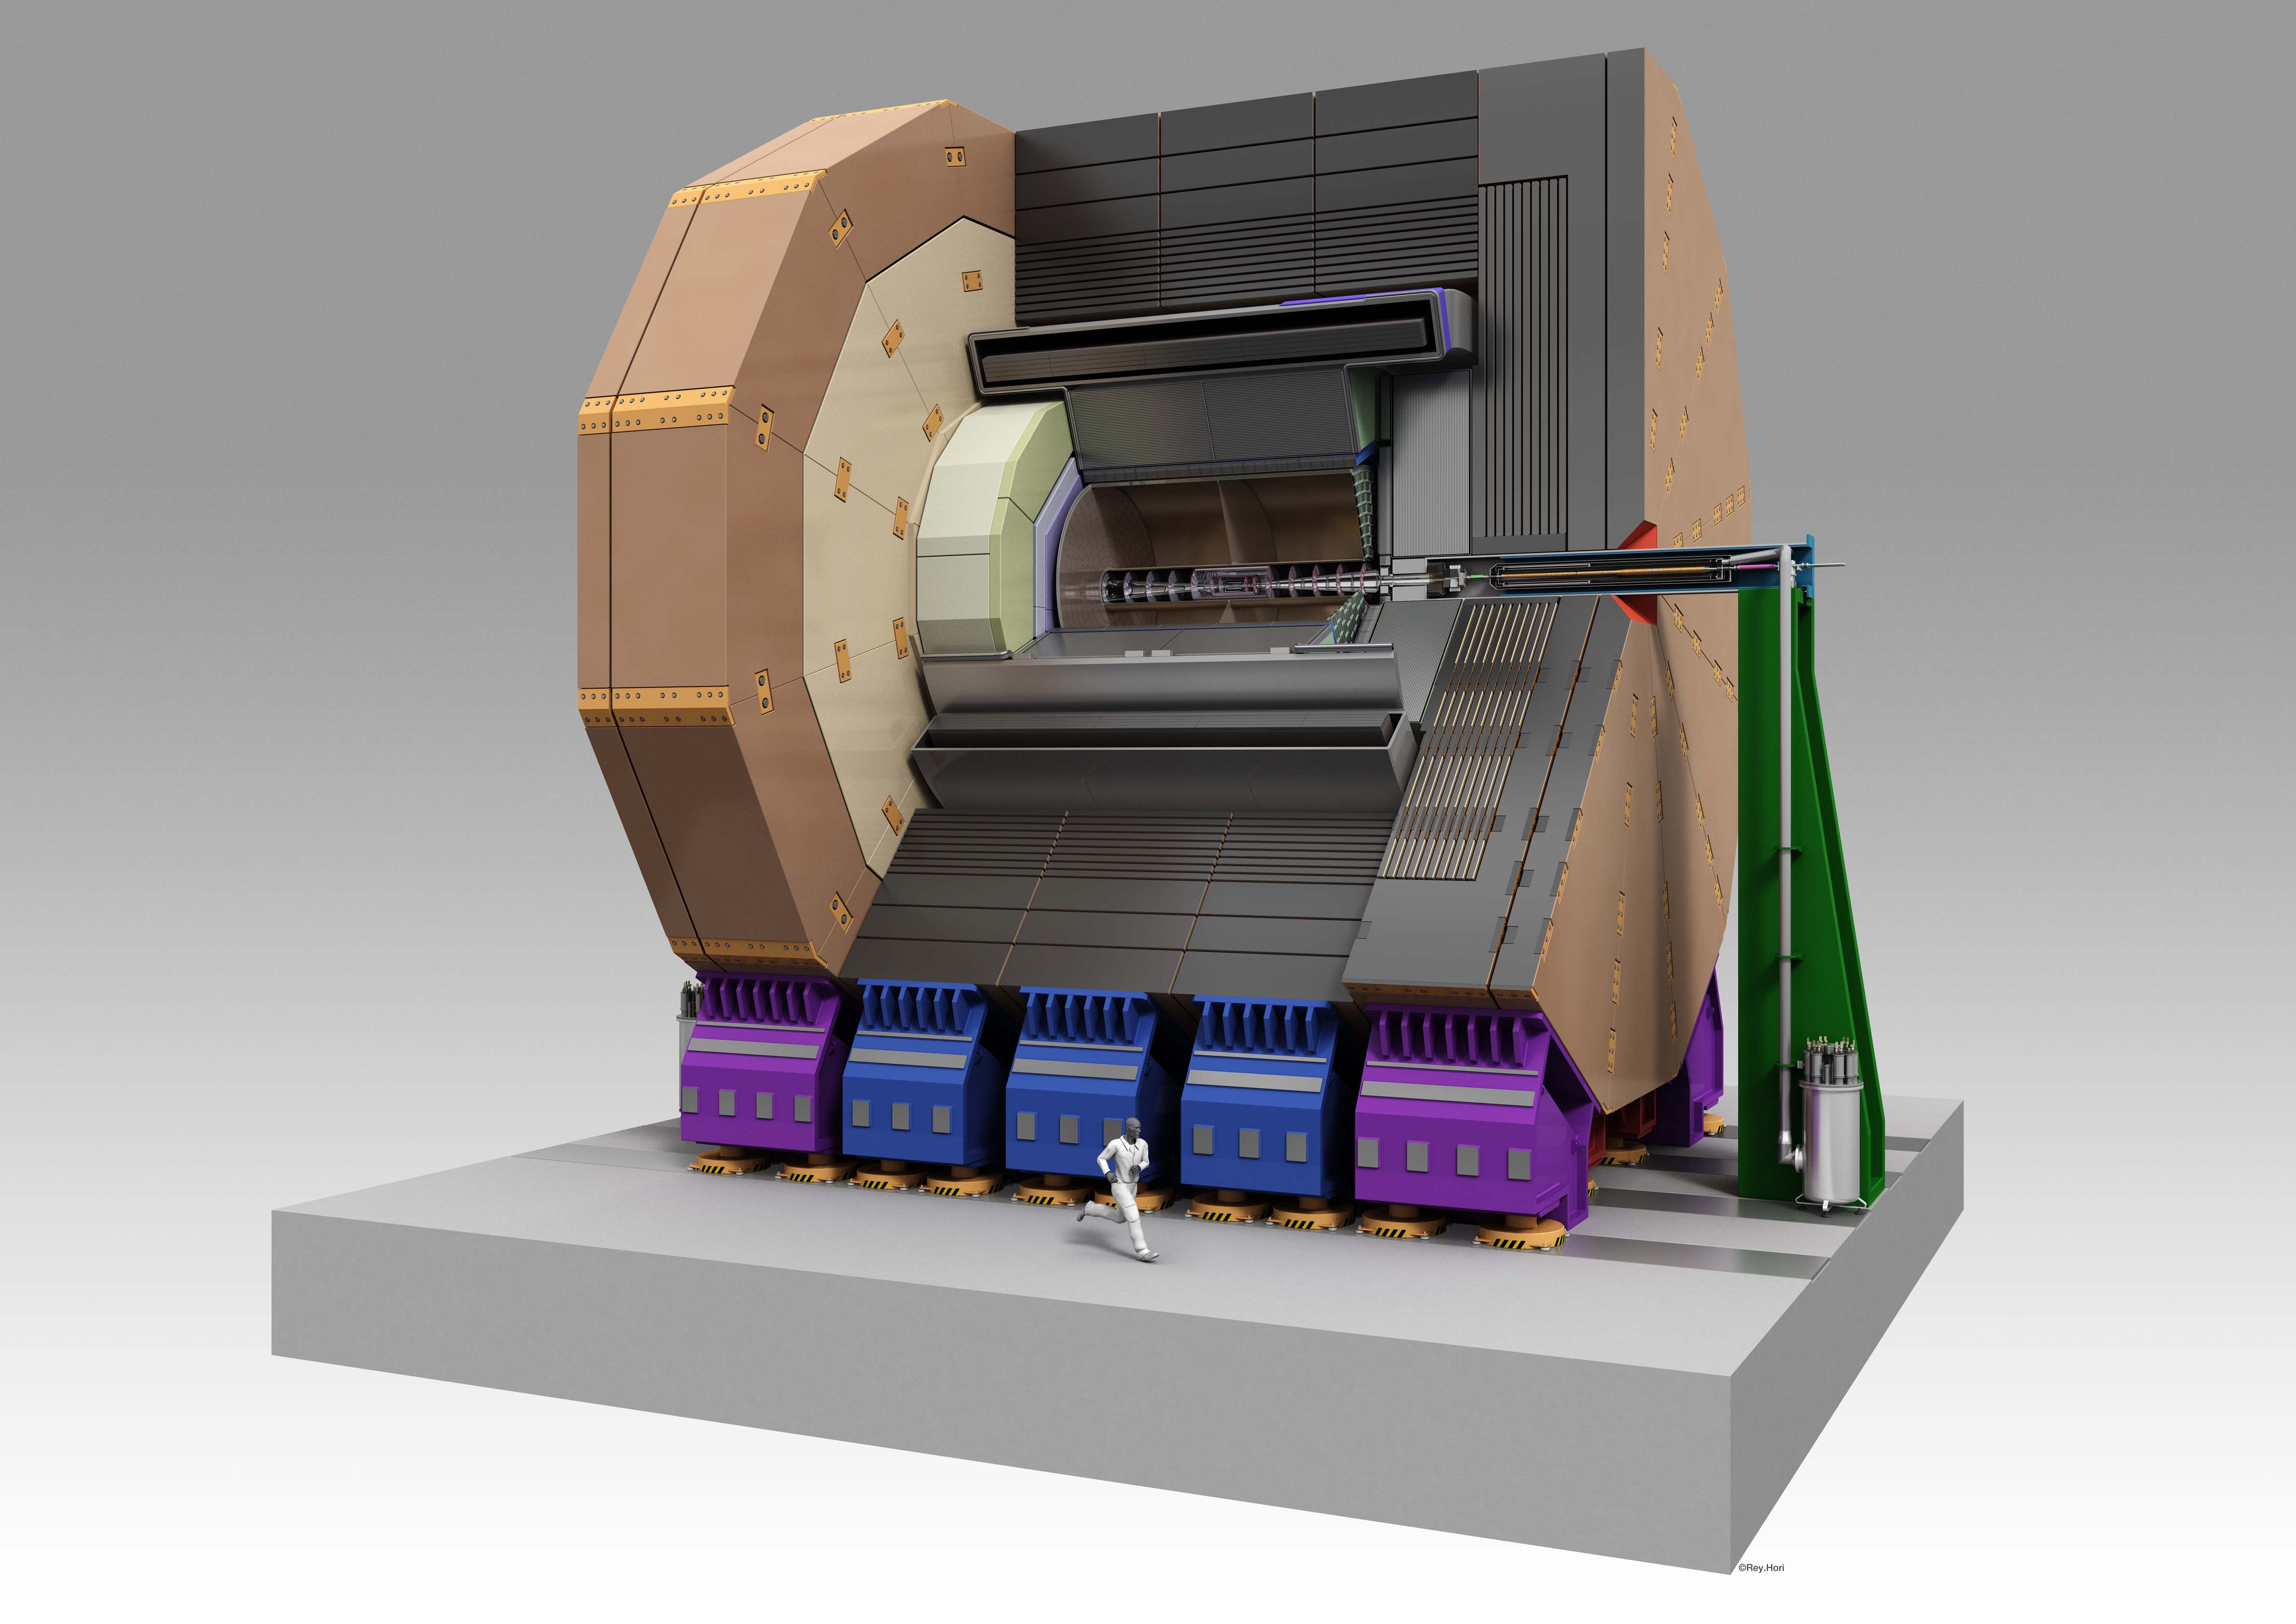
\includegraphics[width=0.48\linewidth]{figs/ild.jpg} ~~~~
    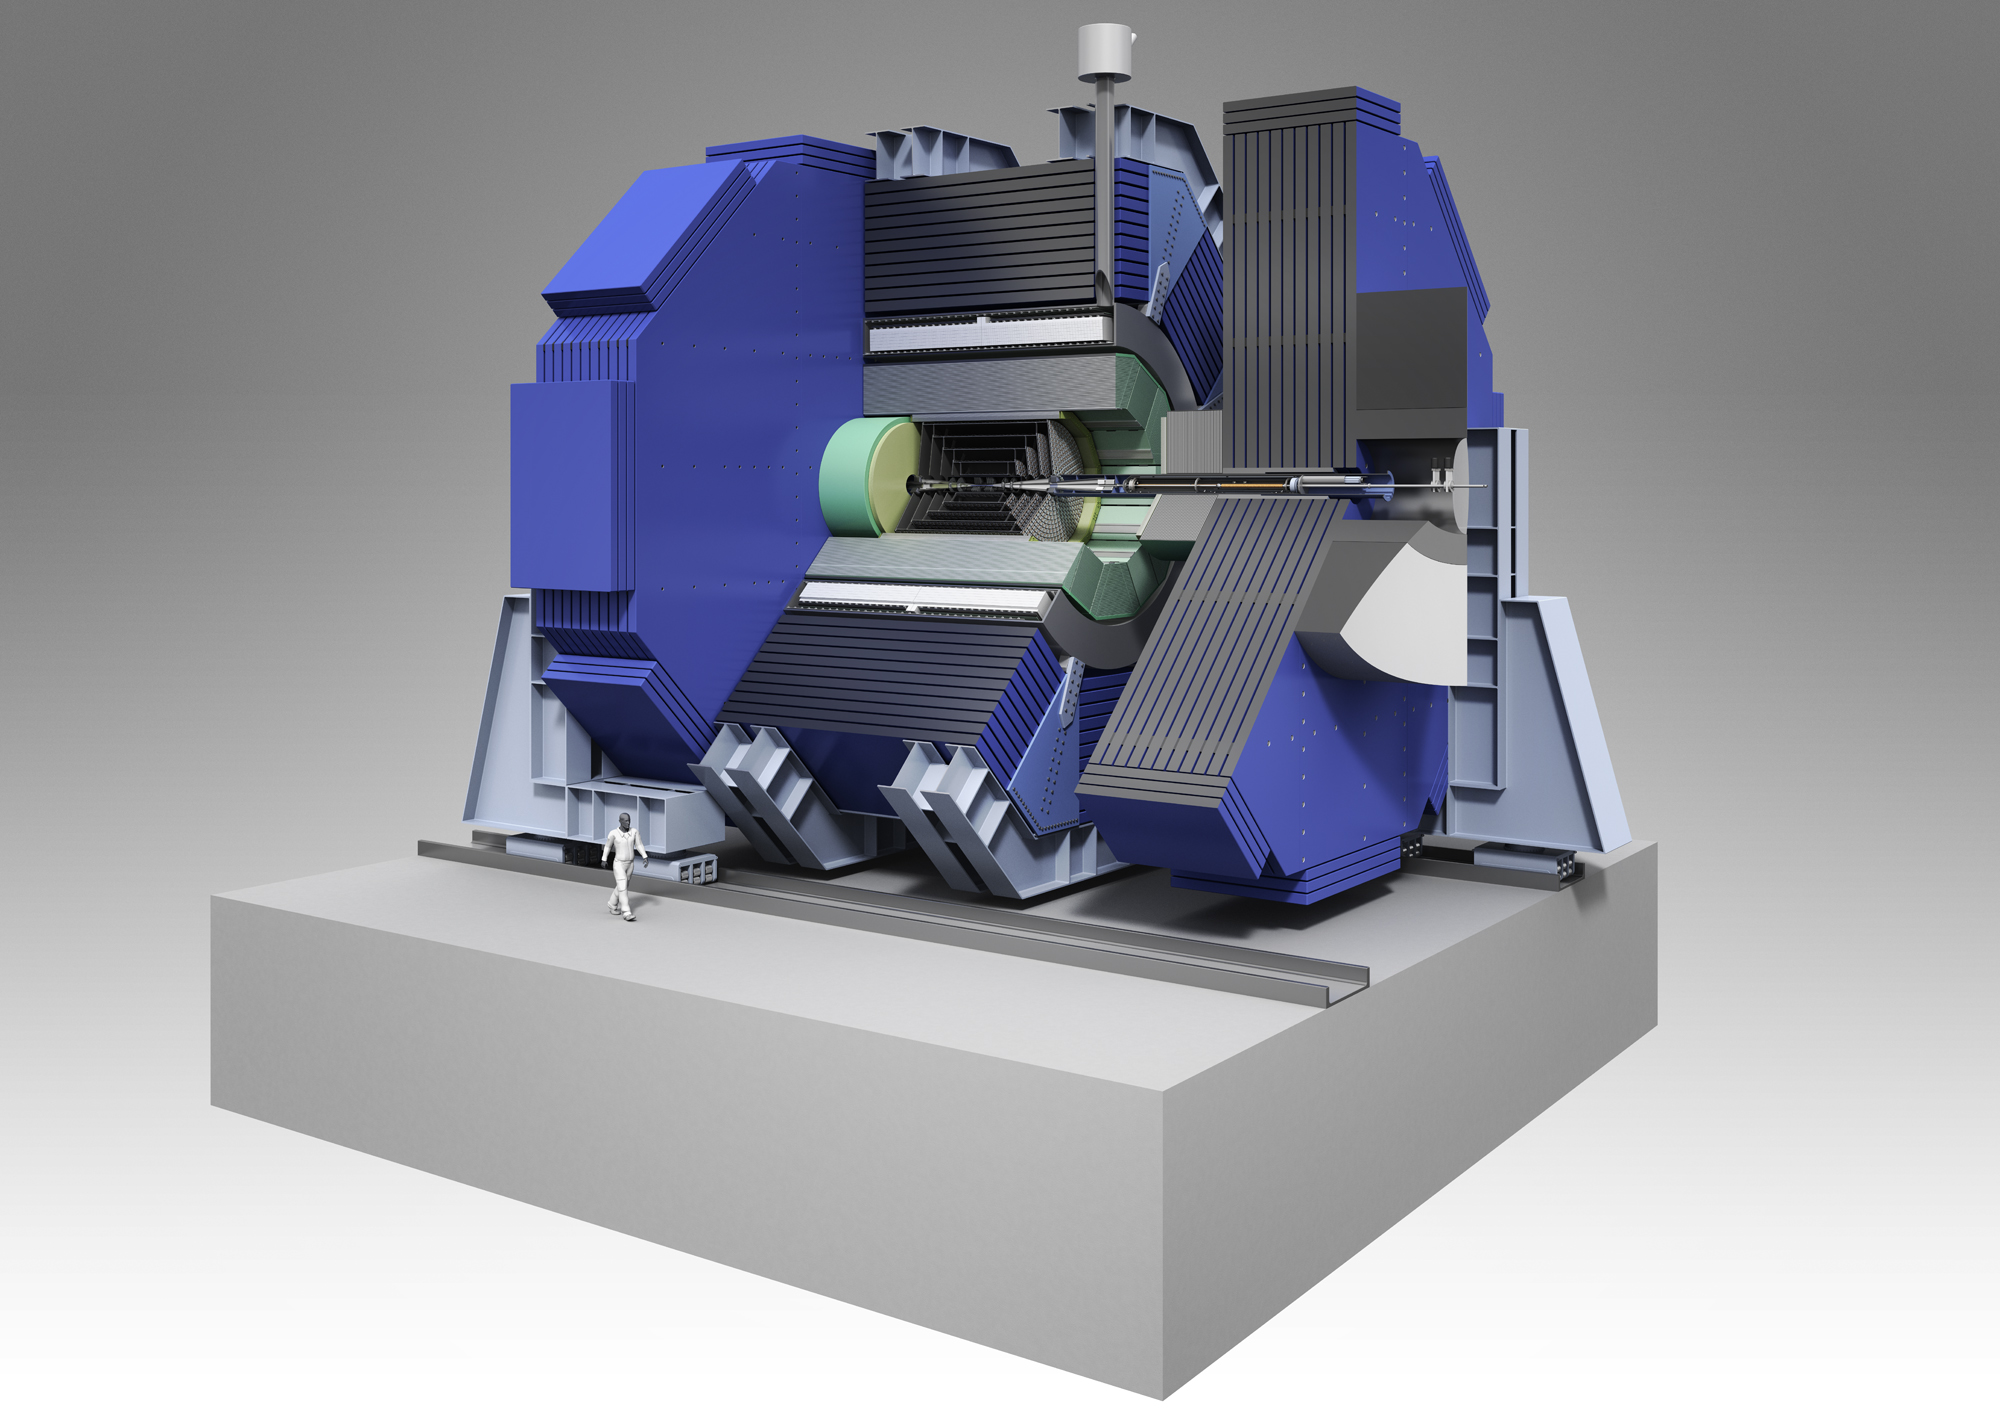
\includegraphics[width=0.48\linewidth]{figs/sid.jpg}
  \end{frame}


  %% Les sous détecteurs
  \begin{frame}
  \frametitle{\secname}
  \framesubtitle{Les sous détecteurs de l'ILD}
    \begin{minipage}{0.62\linewidth}
      \begin{table}
        \begin{tabular}{c|c|c}
          \hline
          \multicolumn{1}{c}{Détecteur} & \multicolumn{1}{c}{Mesure} & \multicolumn{1}{c}{Performance} \\ 
          \hline \hline
          Trajectographe & 1 / $\delta_p$                           & 10$^{-5}$ (GeV/c)$^{-1}$ \\
          Tracking + Calo (jet)   & $\frac{\Delta E}{E}$                     & 3-4 \% \\
          \multirow{3}{*}{Vertex}         & {\footnotesize Résolution spatial}       & {\footnotesize < 3 $\mu m$} \\
          ~              & {\footnotesize Budget matière}           & {\footnotesize < 0.15 \% $X_{0}$/layer} \\
          ~              & {\footnotesize Rayon premier layer}      & {\footnotesize $\simeq$ 1.6 $cm$}
        \end{tabular}
      \end{table}
    \end{minipage} \hfill
    \begin{minipage}{0.36\linewidth}
      \begin{tikzpicture}
        \node[anchor=south west,inner sep=0] at (0,0) {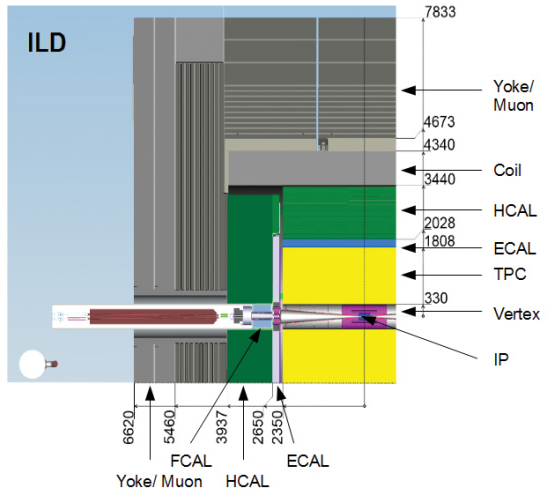
\includegraphics[width=\linewidth]{figs/ild_vue_en_coupe.png}};
        \draw<2>[red,  thick, overlay] (1.95,1.8) -- (2.8,1.8) -- (2.8,2.2) -- (1.6,2.2) -- (1.6,1.4) -- (1.95,1.4) -- (1.95,1.8);
      \end{tikzpicture}
    \end{minipage}
    \begin{minipage}[h]{0.5\linewidth}
      \begin{block}{Des calorimètres pour le suivi de particules}
        \begin{itemize}
          \item ECAL (résolution $\simeq 12\%/\sqrt{E}$) :
          \begin{itemize}
            \item SiWECal : 5 x 5 $mm^2$
            \item ScWECal : 5 x 45 $mm^2$ + SSA
          \end{itemize}
          \item HCAL (résolution $\simeq 60\%/\sqrt{E}$) :
          \begin{itemize}
            \item AHCAL : 3 x 3 $cm^2$
            \item SDHCAL : 1 x 1 $cm^2$
          \end{itemize}
        \end{itemize}
      \end{block}
      \crefarticle{ILC Technical Design Report, Vol.4 Detectors \\}{arXiv:1306.6329}
    \end{minipage} \hfill
    \begin{minipage}[h]{0.48\linewidth}
      \begin{tikzpicture}
        \node[anchor=south west,inner sep=0] at (0,0) {\includegraphics[width=0.8\linewidth]{figs/pfa_event_display.png}};
        \draw<2>[red,  thick, overlay] (1.9,1.6) -- (1.9,0) -- (0,0) -- (0,3.62) -- (3.9,3.62) -- (1.9,1.6);
      \end{tikzpicture}
    \end{minipage}
  \end{frame}

  %% Le prototype SDHCAL
  \subsection{Le calorimètre hadronique semi-digital}

  \begin{frame}
  \frametitle{\secname}
  \framesubtitle{\subsecname}
    \begin{minipage}{0.52\linewidth}
      \begin{block}{Semi-Digital Hadron Calorimeter}
        \begin{itemize}
          \item Calorimètre à échantillonnage
          \item 48 plans :
          \begin{itemize}
            \item Absorber en acier
            \item Milieu sensitif : GRPC
          \end{itemize}
          \item Segmentation :
          \begin{itemize}
            \item Transverse : 1 $cm^2$
            \item Longitudinale : 2.67 cm (abs. + sens)
          \end{itemize}
          \item Lecture semi-digitale à 3 seuils
          \begin{itemize}
            \item \textcolor{MyGreen}{seuil 1} : peu de particules
            \item \textcolor{blue}{seuil 2} : quelques particules
            \item \textcolor{red}{seuil 3} : beaucoup de particules
          \end{itemize}
        \end{itemize}
      \end{block}
      \crefarticle{The Calice Collaboration}{arXiv:1602.02276}
    \end{minipage} \hfill
    \begin{minipage}{0.46\linewidth}
      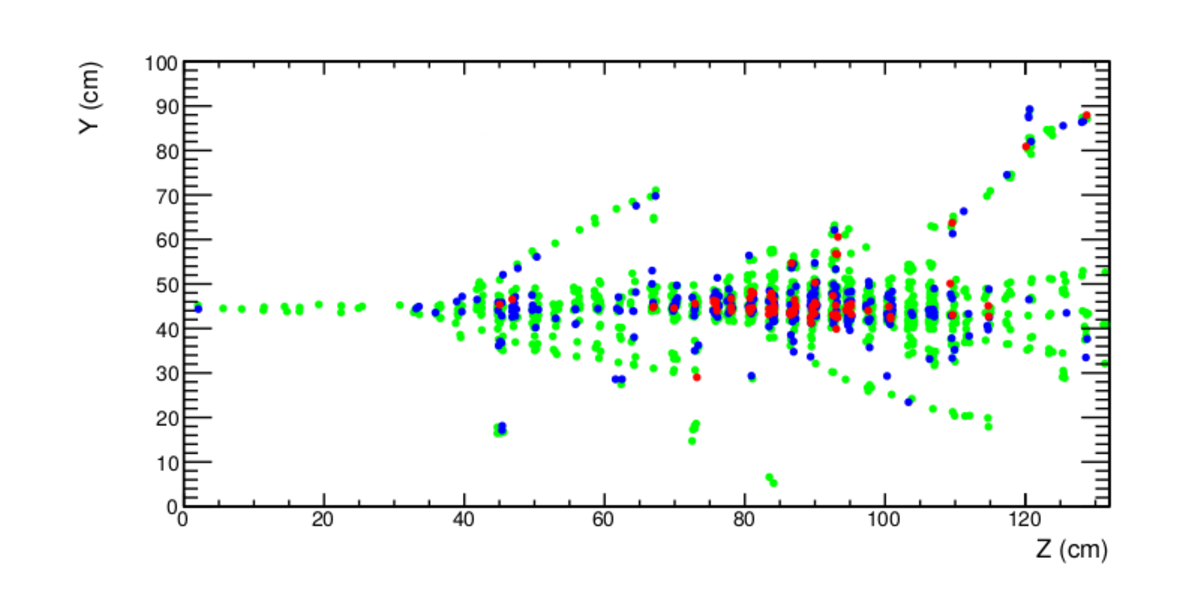
\includegraphics[width=\linewidth]{figs/sdhcal_pion_80GeV.pdf}
    \end{minipage}
    \begin{minipage}{0.58\linewidth}
      \begin{center}
        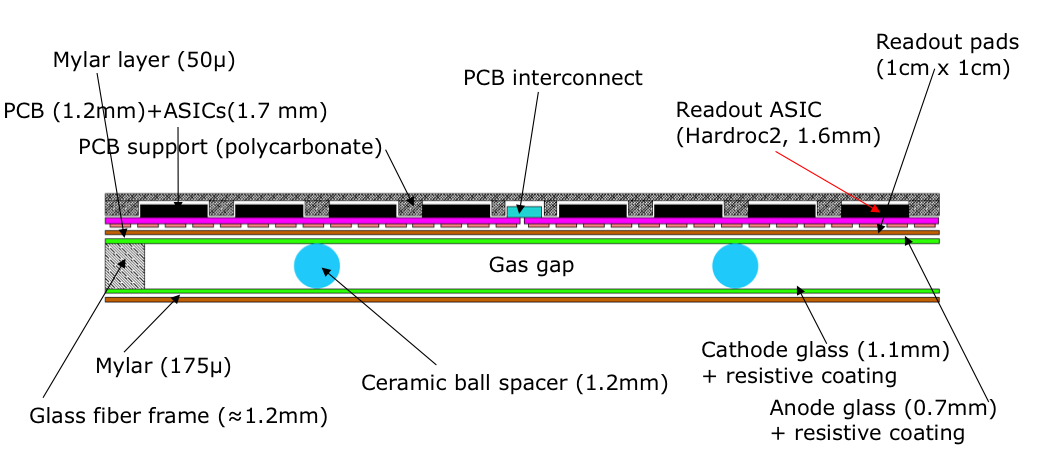
\includegraphics[width=0.9\linewidth]{figs/GRPC-K7.png}
      \end{center}
    \end{minipage} \hfill
    \begin{minipage}{0.4\linewidth}
      \begin{center}
        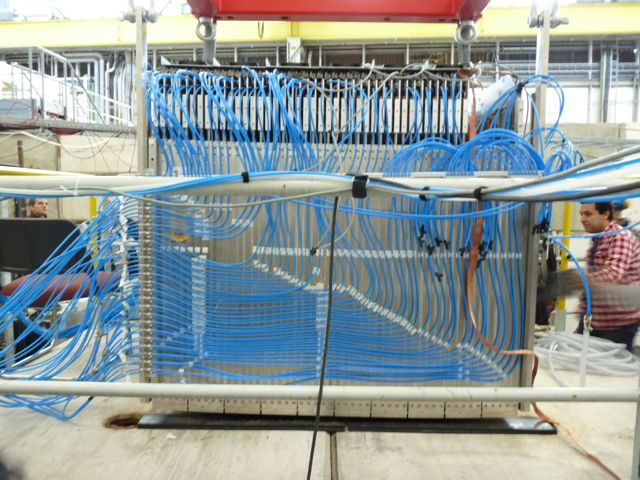
\includegraphics[width=0.7\linewidth]{figs/sdhcal_testbeam.jpg}
      \end{center}
    \end{minipage}
  \end{frame}


  %% Performances du SDHCAL
  \subsection{Performances du SDHCAL}

  %% Multiplicité / Efficacité
  \begin{frame}
  \frametitle{\secname}
  \framesubtitle{\subsecname}
    \begin{minipage}{0.5\linewidth}
      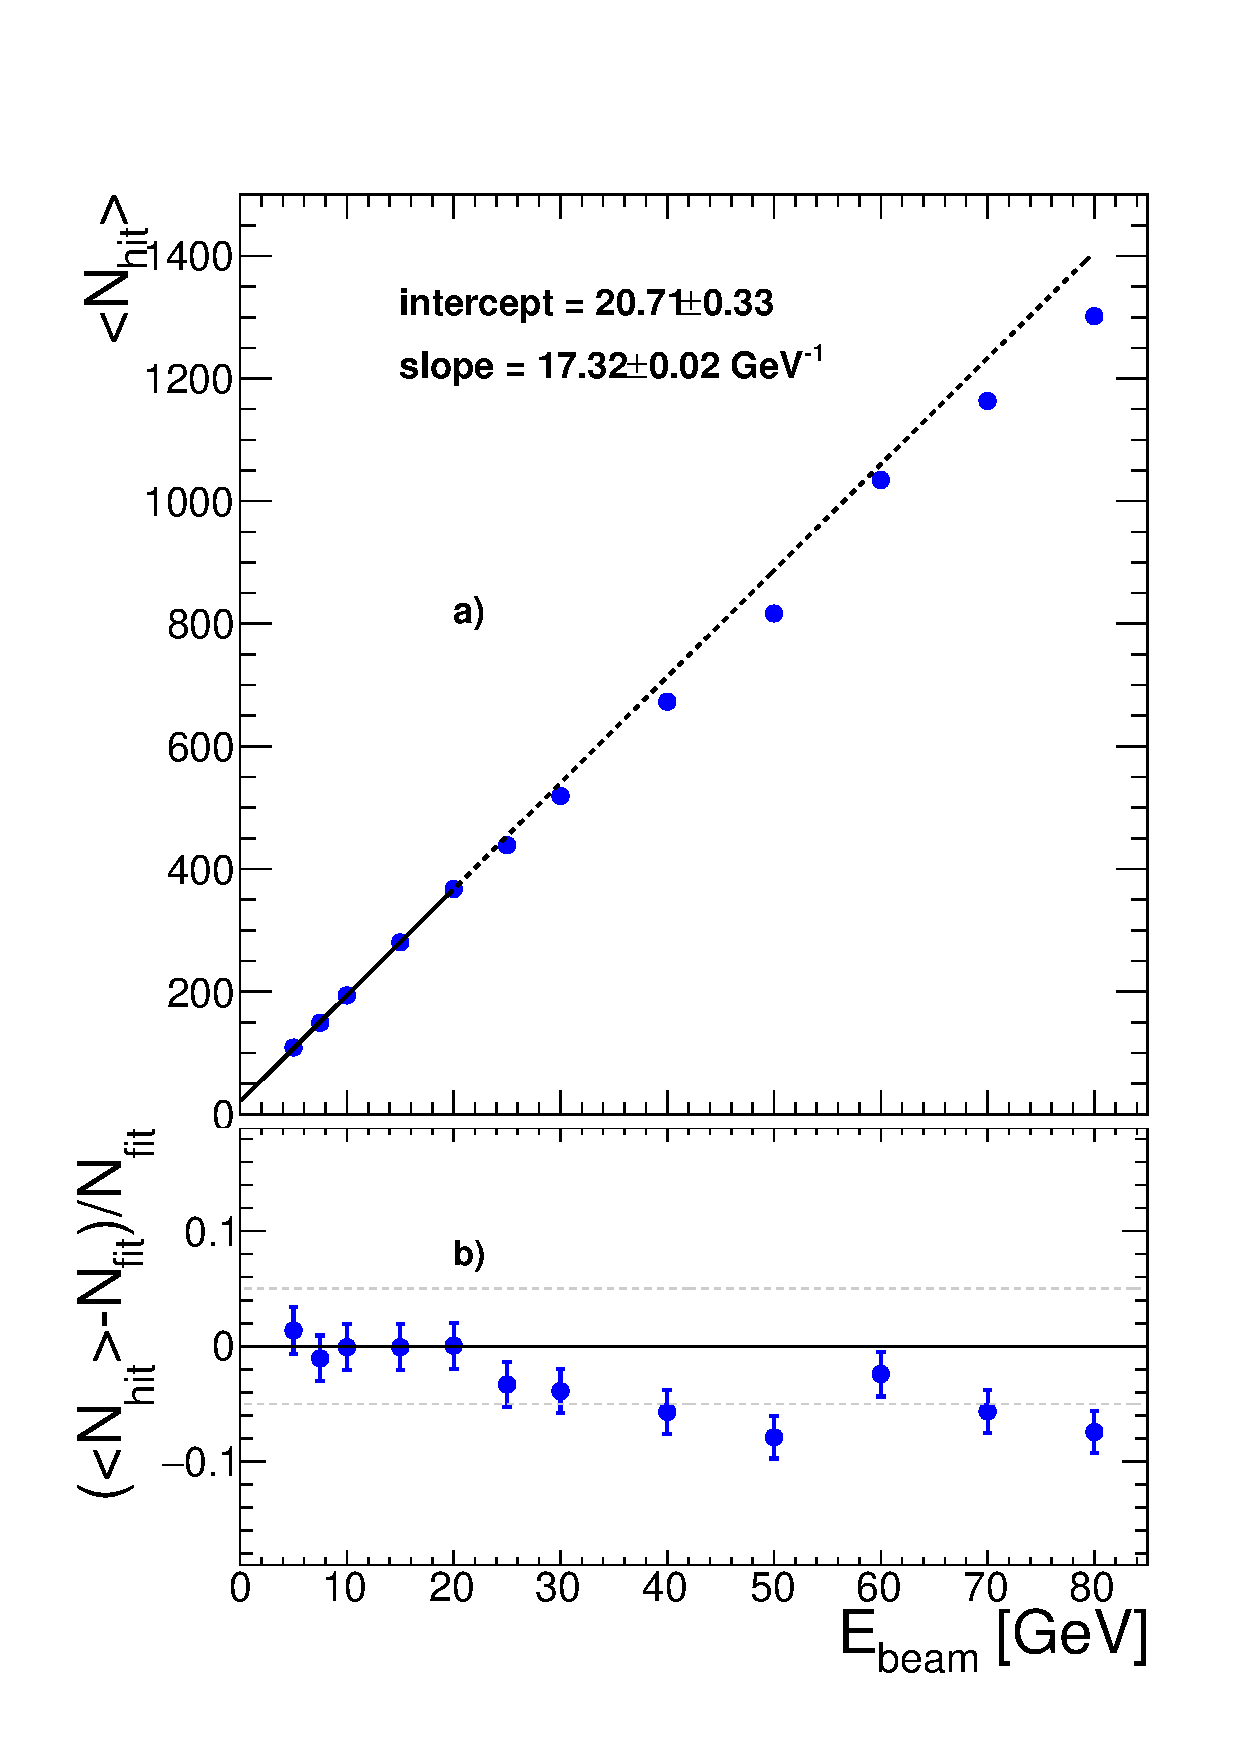
\includegraphics[width=1\linewidth]{figs/NHITPION.pdf}
    \end{minipage} \hfill
    \begin{minipage}{0.48\linewidth}
      \begin{center}
        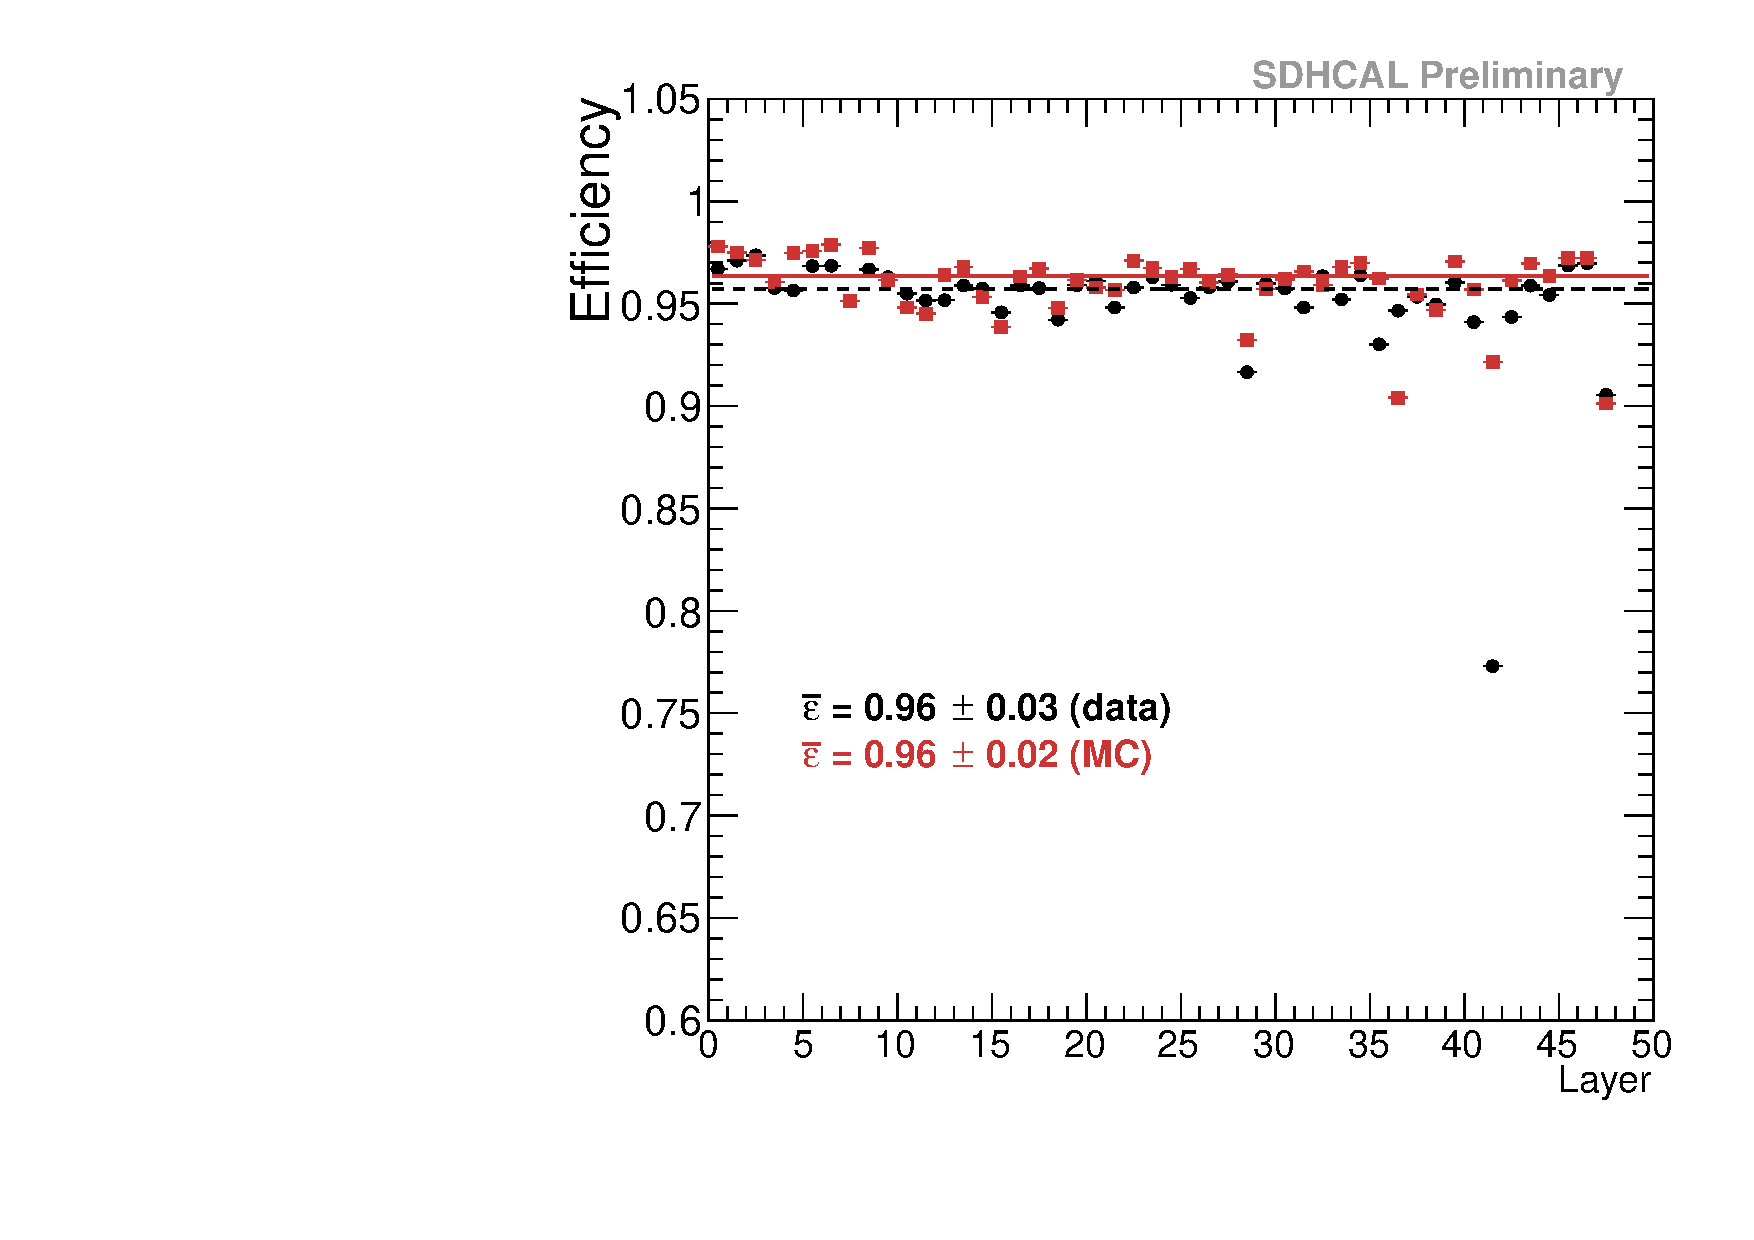
\includegraphics[width=0.7\linewidth]{figs/effLayer.pdf} \\
        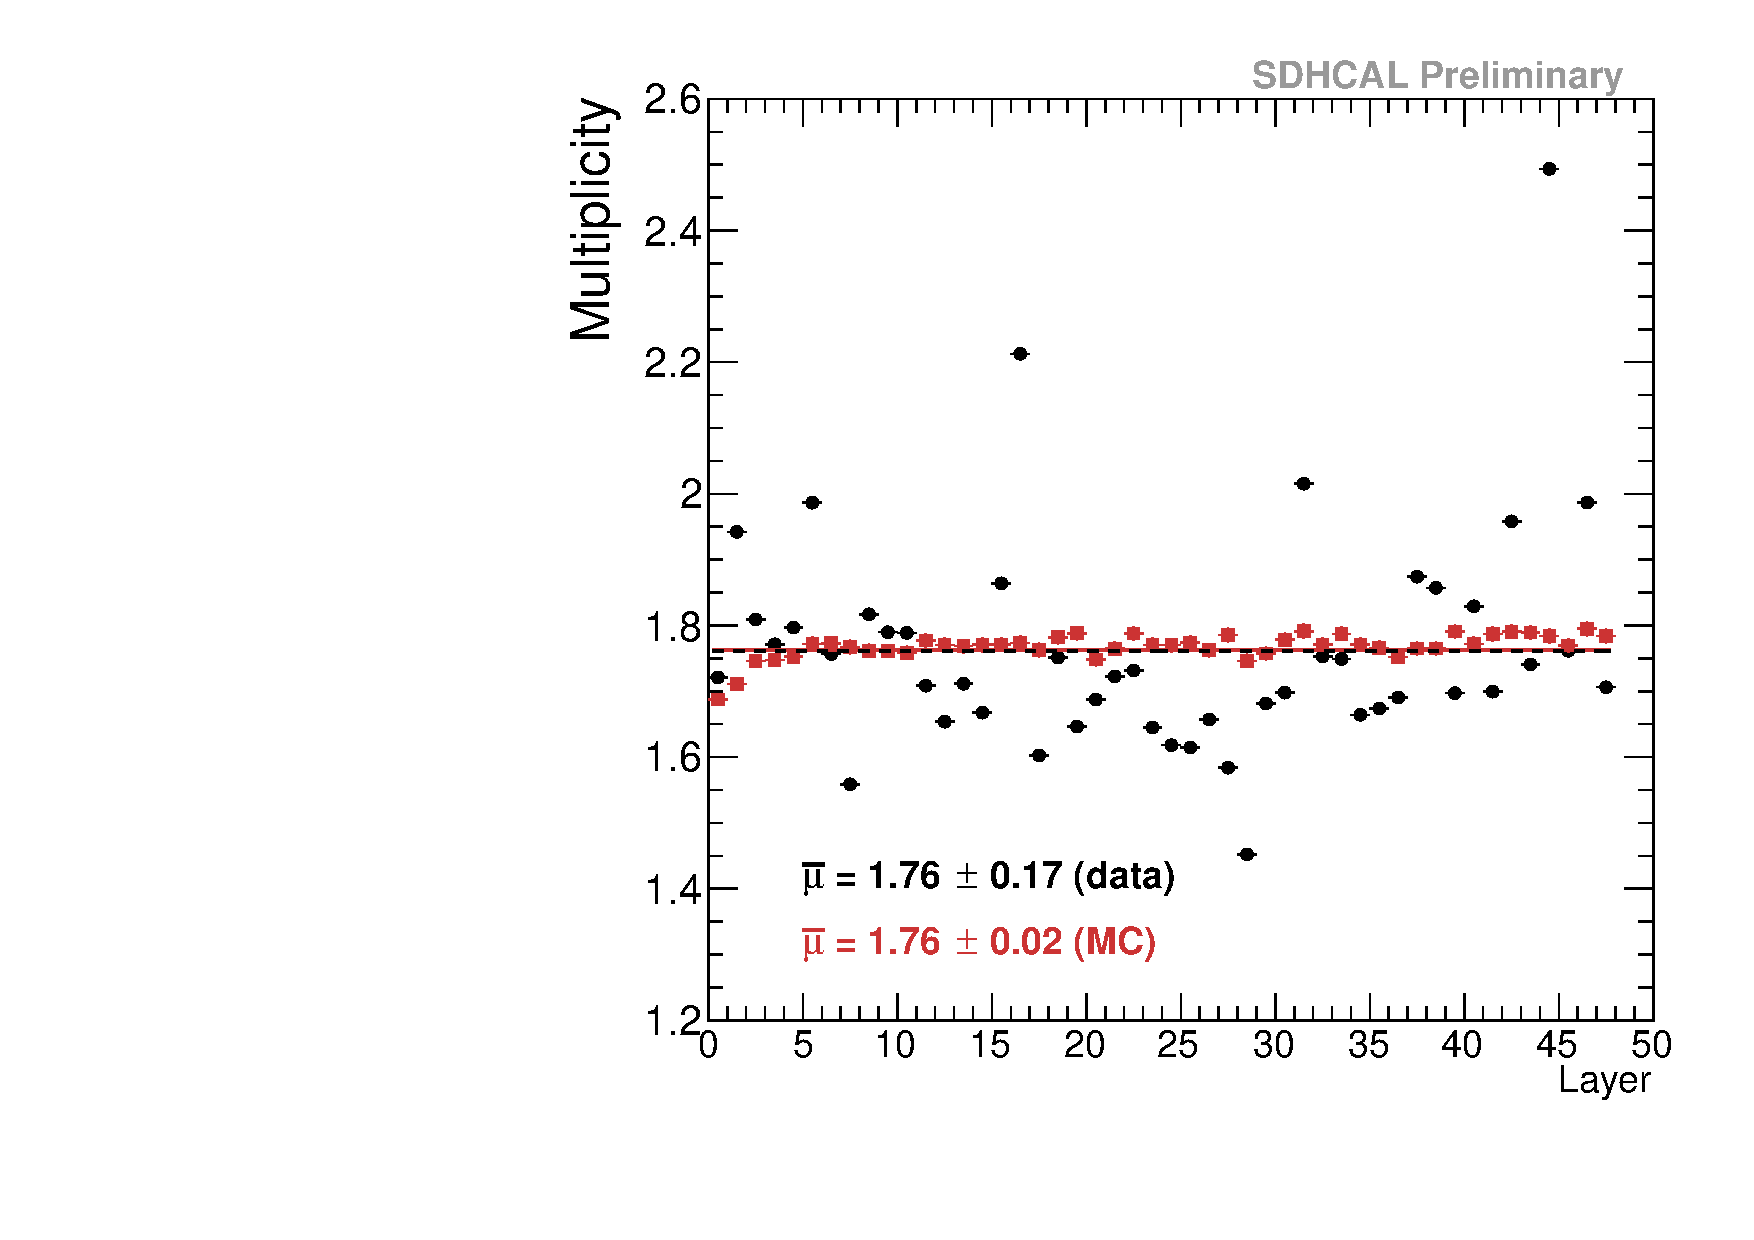
\includegraphics[width=0.7\linewidth]{figs/mulLayer.pdf}
      \end{center}
    \end{minipage}
    \crefarticle{The Calice Collaboration}{arXiv:1604.04550}
  \end{frame}


  %% Reconstruction de l'énergie
  \begingroup
  \small
  \begin{frame}
  \frametitle{\secname}
  \framesubtitle{\subsecname - reconstruction de l'énergie des hadrons}

    \begin{minipage}{0.65\linewidth}

      Principales observables du SDHCAL : $N_{hit}$, \textcolor{MyGreen}{$N_1$}, \textcolor{blue}{$N_2$}, \textcolor{red}{$N_3$} \\

      Reconstruction de l'énergie des hadrons : \\
      $\rightarrow$ plusieurs estimateurs possibles !

      \pause
      \begin{block}{Formule linéaire}
        \begin{equation}
          E = \alpha\cdot \textcolor{MyGreen}{N_1} + \beta\cdot \textcolor{blue}{N_2} + \gamma\cdot \textcolor{red}{N_3}
        \end{equation}
        avec $\alpha$, $\beta$ et $\gamma$ trois constantes.
        \begin{itemize}
          \item[\textcolor{MyGreen}{$\checkmark$}] Application très simple aux techniques de \textit{PFA}
          \item[\textcolor{red}{$\times$}] Mauvaise linéarité à basse énergie
        \end{itemize}
      \end{block}

      \pause
      \begin{block}{Formule quadratique}
        \begin{equation}
          E = \alpha(NHit)\cdot \textcolor{MyGreen}{N_1} + \beta(NHit)\cdot \textcolor{blue}{N_2} + \gamma(NHit)\cdot \textcolor{red}{N_3}
        \end{equation}
        avec :
        \begin{equation}
          \alpha(NHit) = \alpha_1 + \alpha_2\cdot NHit + \alpha_3\cdot NHit^2
        \end{equation}
        \begin{equation}
          \beta(NHit) = \beta_1 + \beta_2\cdot NHit + \beta_3\cdot NHit^2
        \end{equation}
        \begin{equation}
          \gamma(NHit) = \gamma_1 + \gamma_2\cdot NHit + \gamma_3\cdot NHit^2
        \end{equation}
        \begin{itemize}
          \item[\textcolor{MyGreen}{$\checkmark$}] Bonne linéarité et résolution sur toute la gamme en énergie
          \item[\textcolor{red}{$\times$}] Application aux techniques de \textit{PFA} plus complexe
        \end{itemize}
      \end{block}

    \end{minipage} \hfill
    \begin{minipage}{0.3\linewidth}

      \pause
      \begin{tikzpicture}
        \draw[red,  thick, overlay] (-7.8,-7.8) rectangle (-0.3,-3.8);
        \draw[red,  thick, overlay] (-0.1,-7) rectangle (3.5,0);
      \end{tikzpicture}
      \begin{center}
        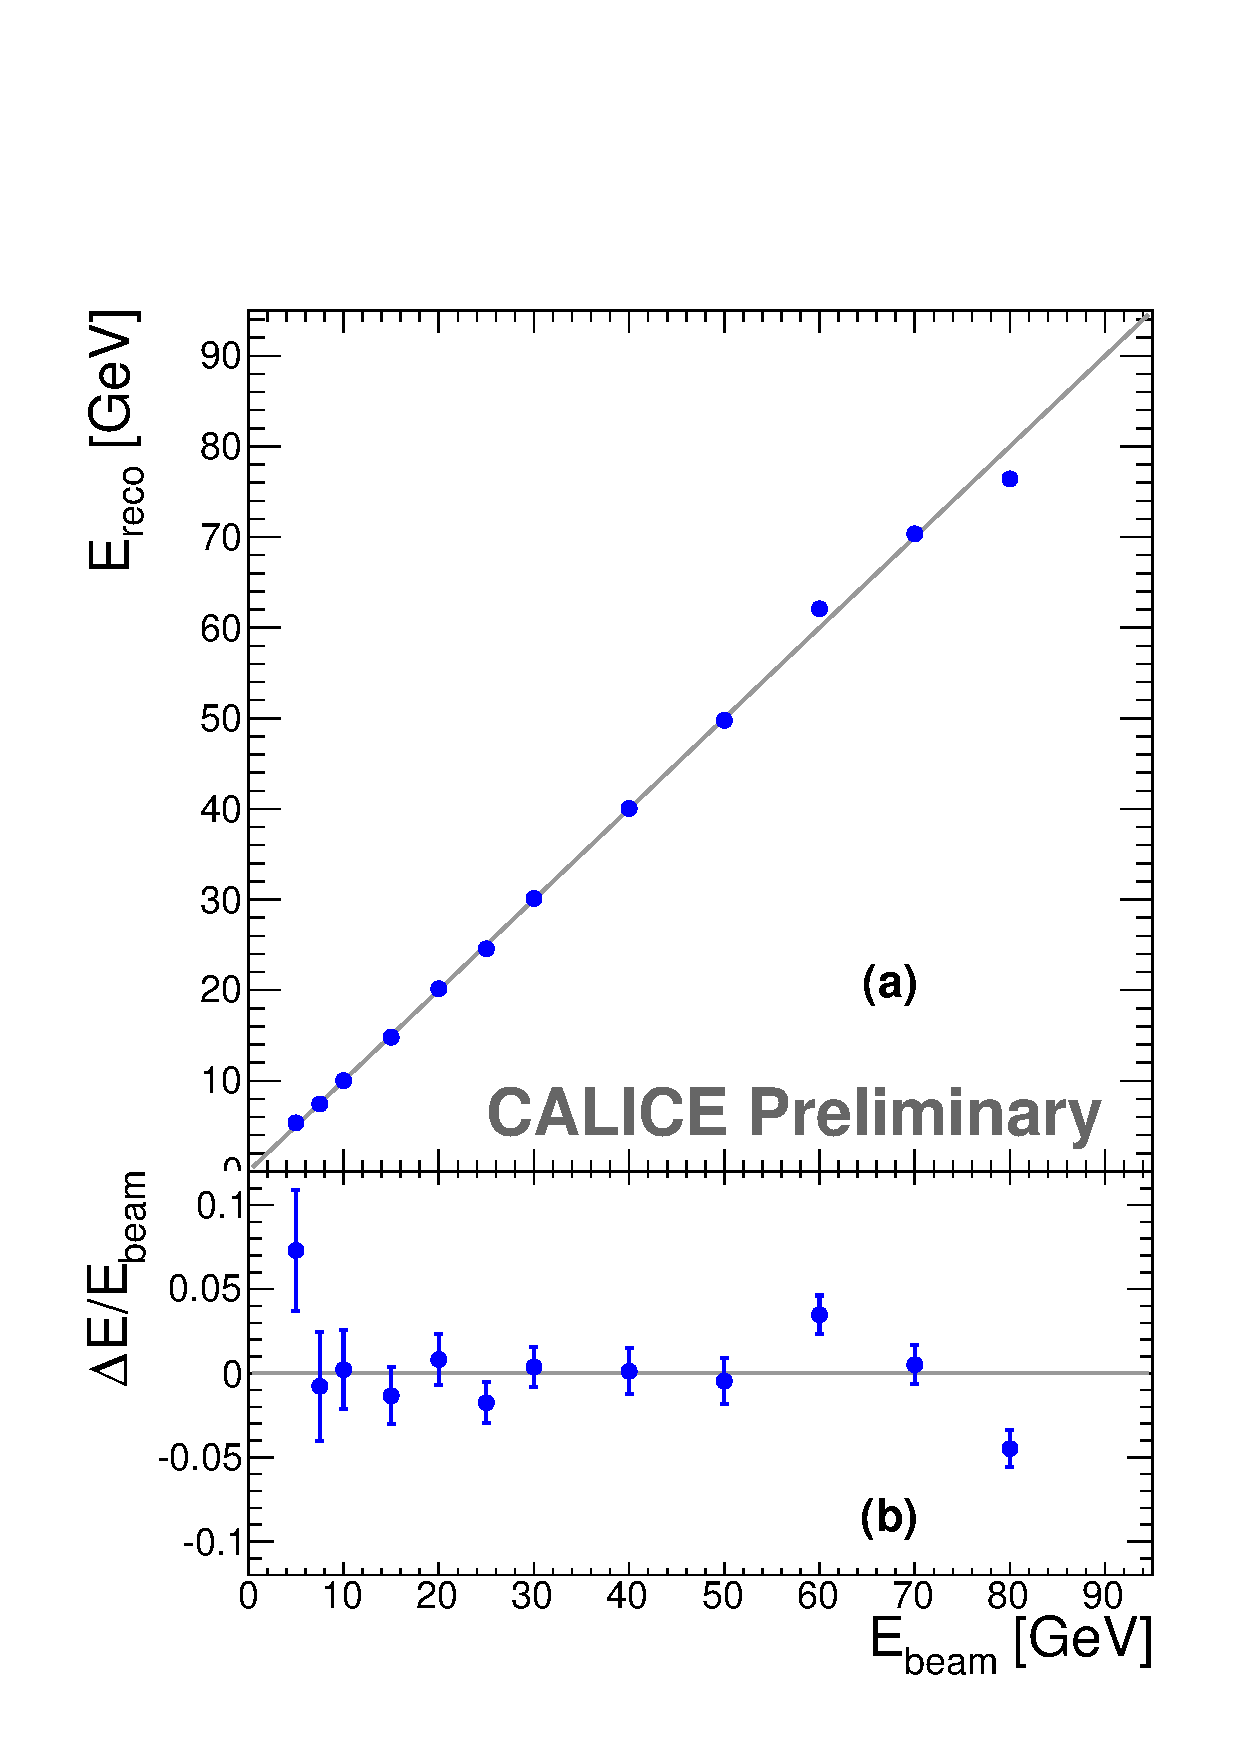
\includegraphics[width=\linewidth]{figs/Energy-Linearity.pdf} \\
        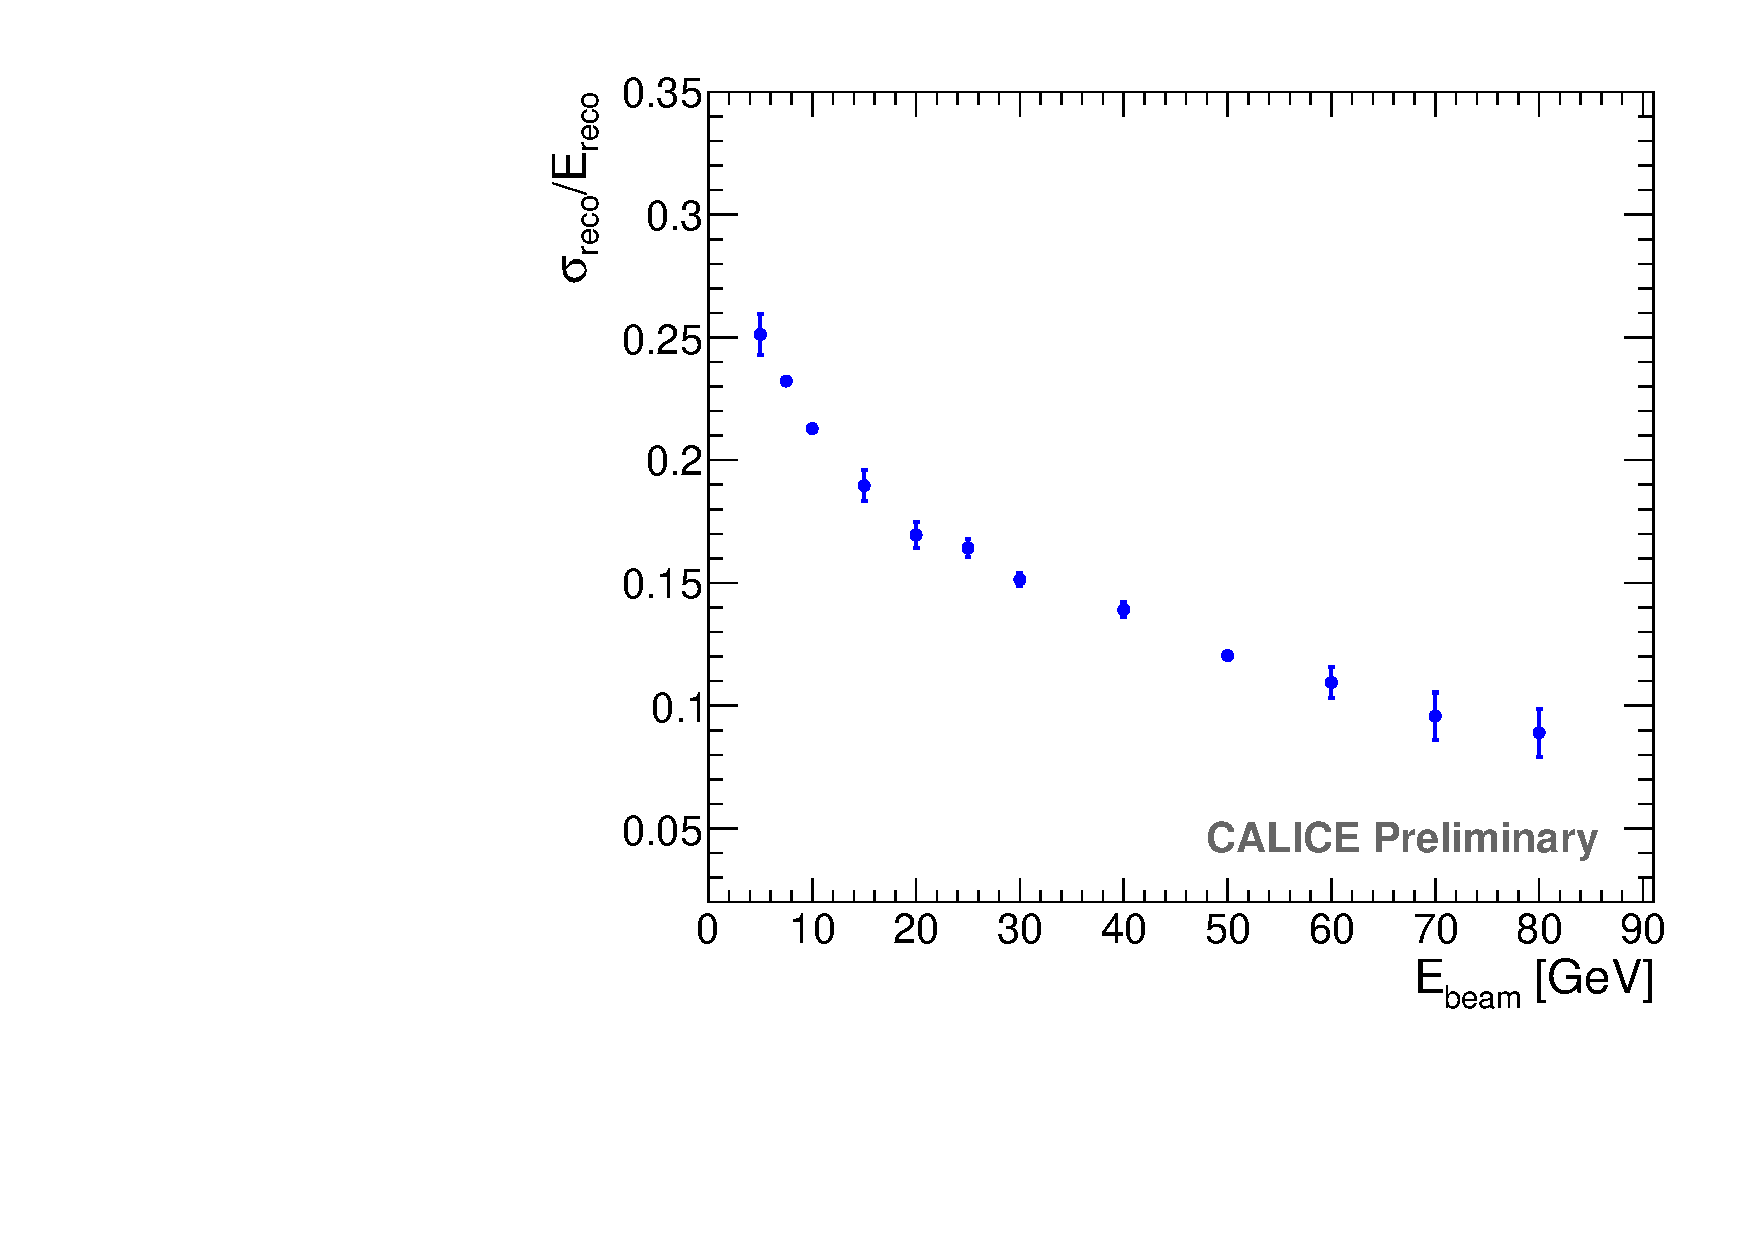
\includegraphics[width=\linewidth]{figs/Energy-Resolution.pdf}
      \end{center}
      \vspace{-0.4cm}
      \crefarticle{The Calice Collaboration}{JINST \textbf{11} P04001}
    \end{minipage}

  \end{frame}
\endgroup

  %% Quelques désaccords (1)
  \begin{frame}
  \frametitle{\secname}
  \framesubtitle{\subsecname - quelques désaccords ...}
    \begin{center}
      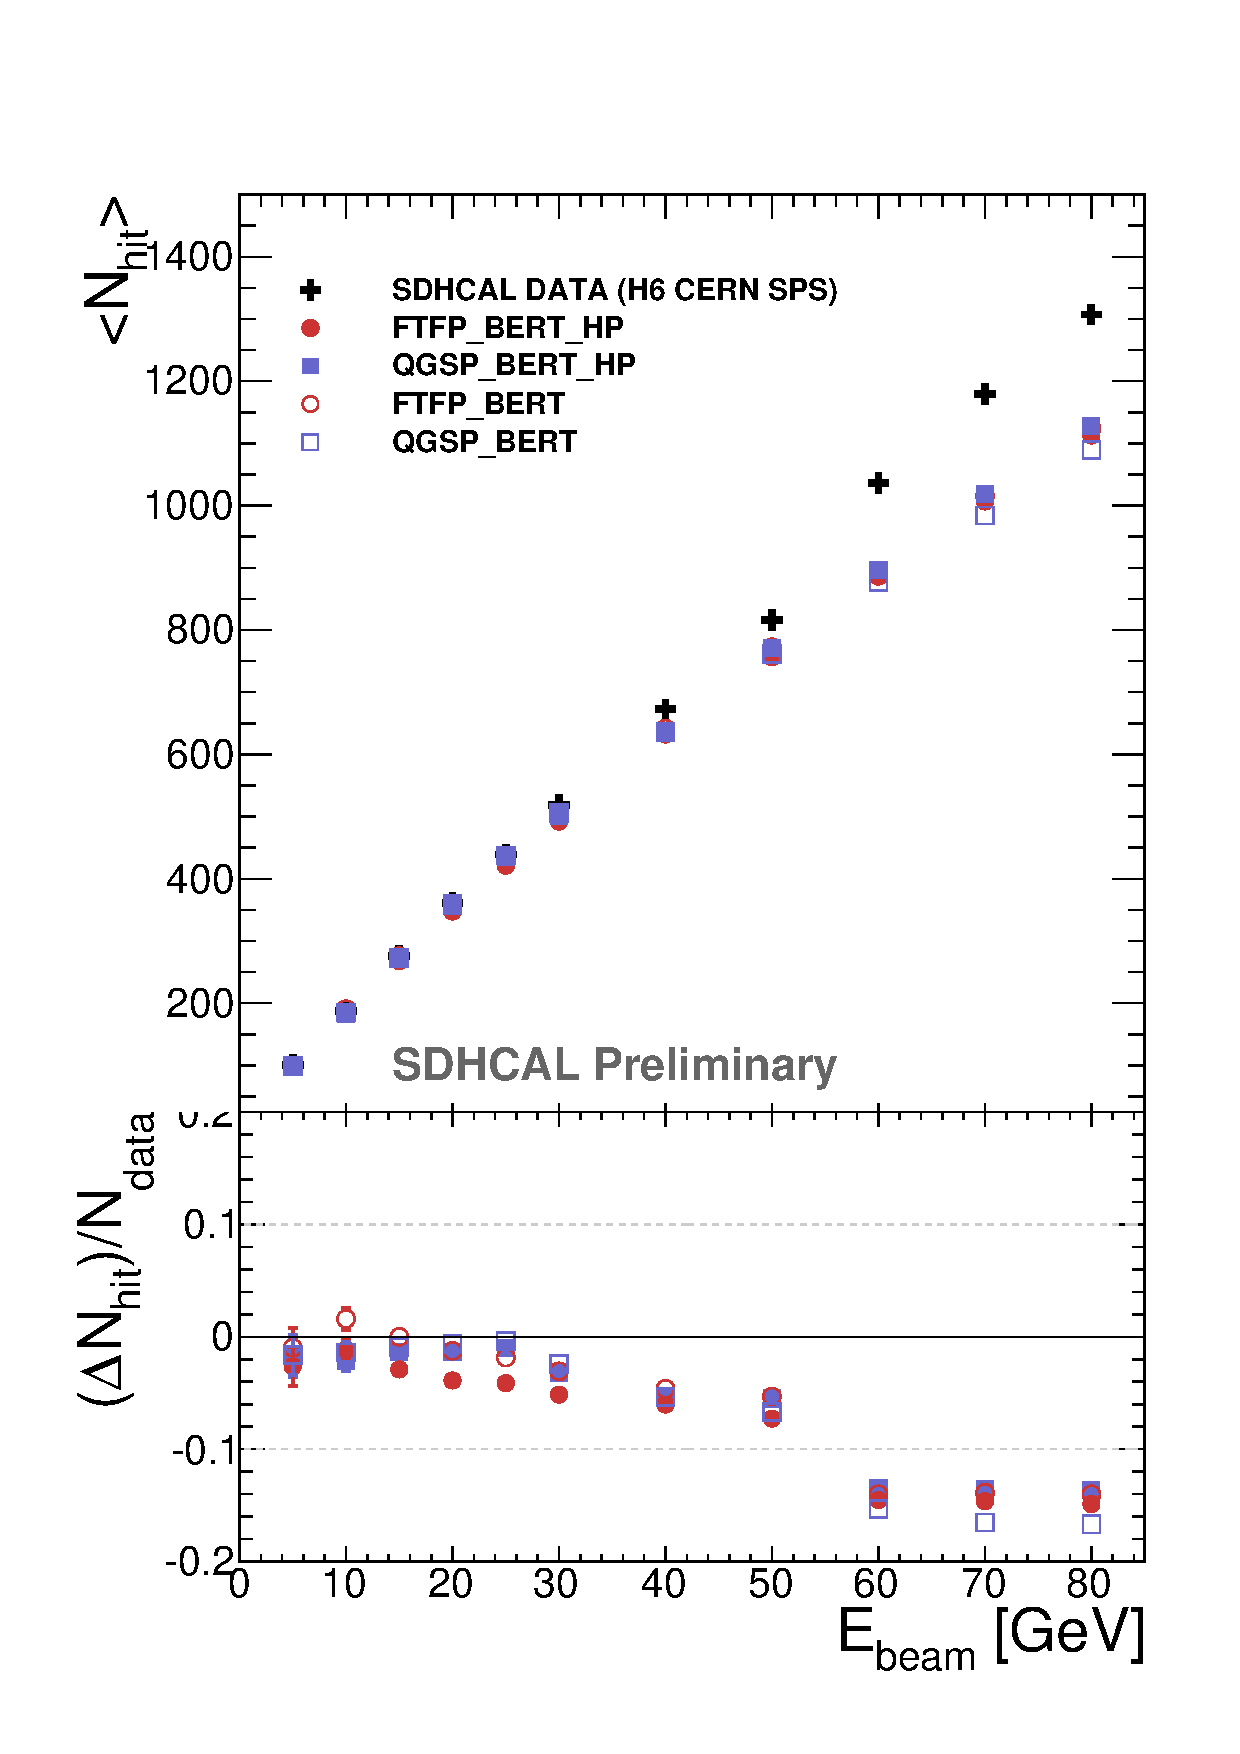
\includegraphics[width=0.49\linewidth]{figs/NHITPIONHP.pdf}
      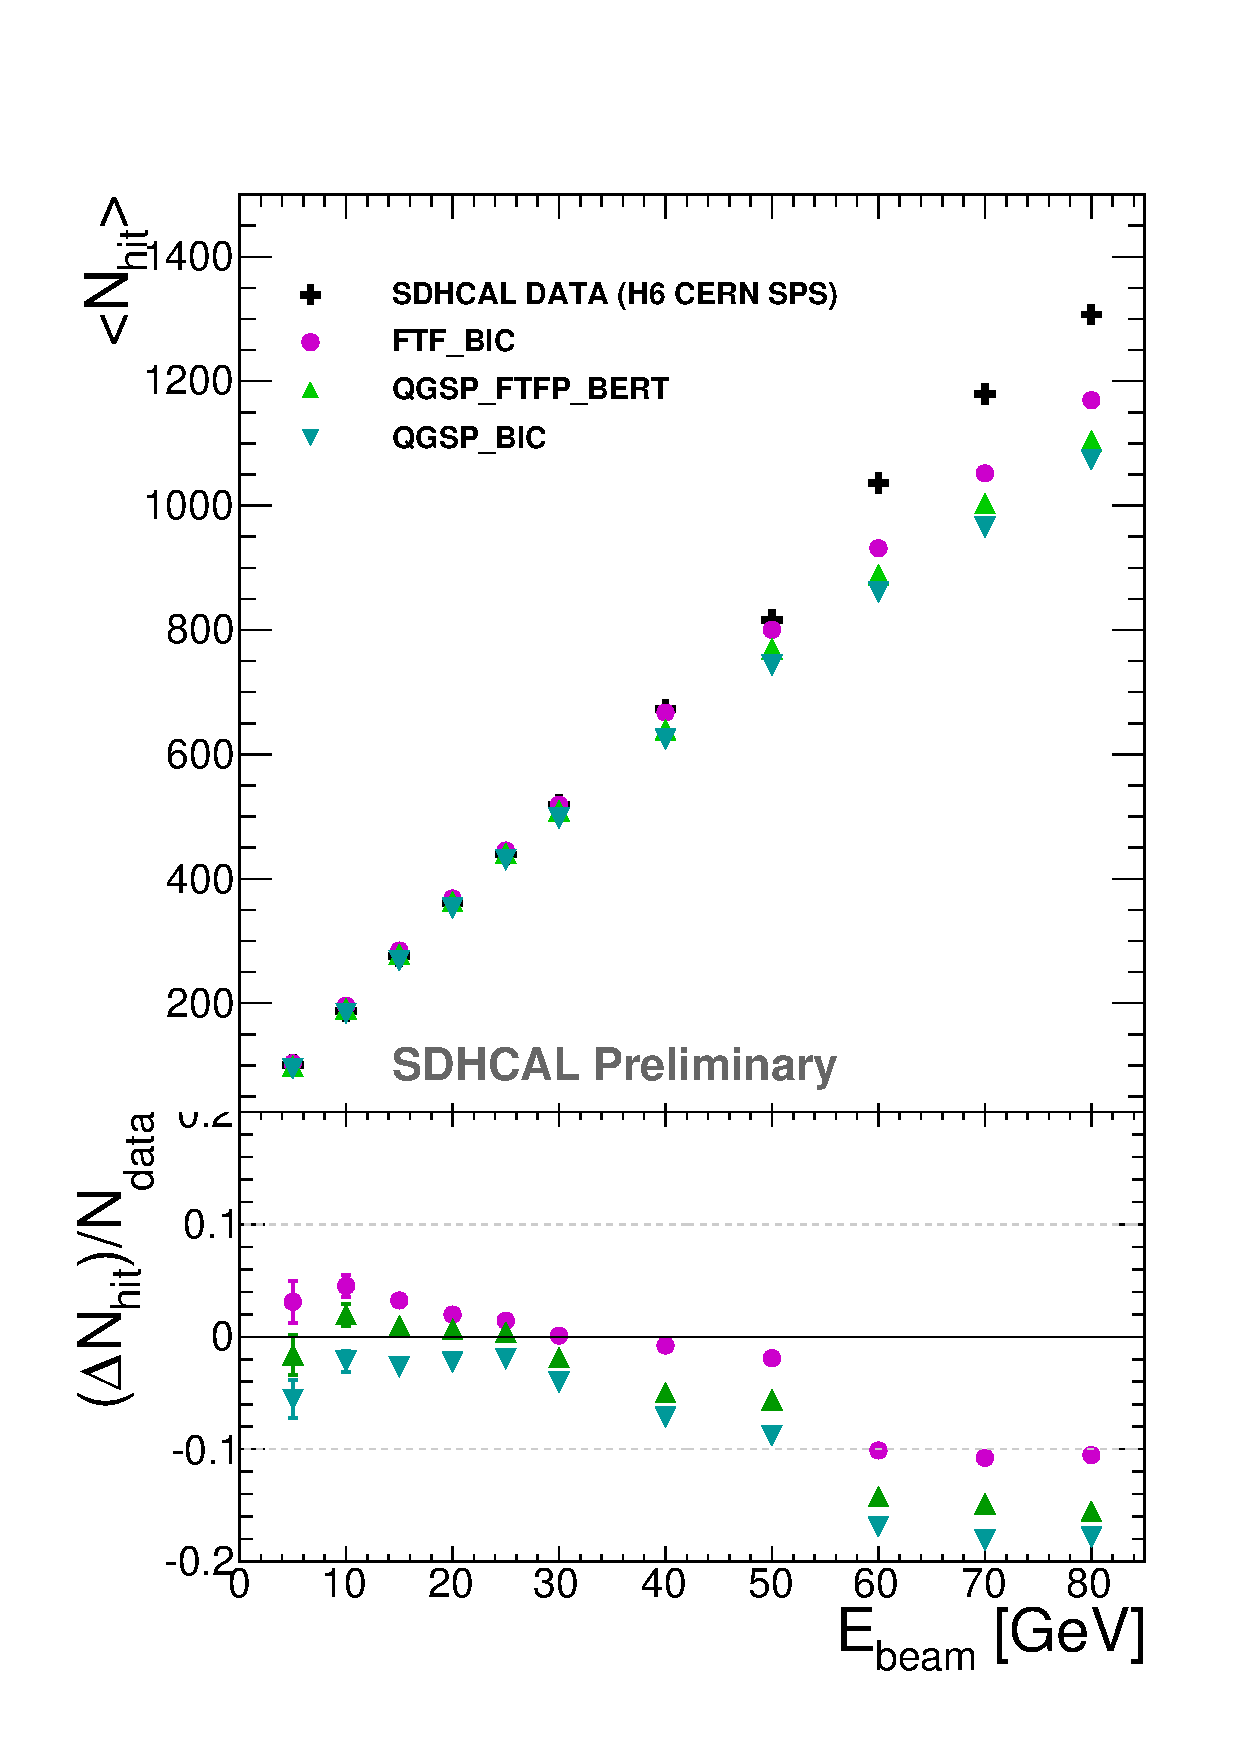
\includegraphics[width=0.49\linewidth]{figs/NHITPION_MODEL.pdf}
    \end{center}
    \crefarticle{Thèse A. Steen}{2015LYO10230}
  \end{frame}


  %% Quelques désaccords (2)
  \begin{frame}
  \frametitle{\secname}
  \framesubtitle{\subsecname - quelques désaccords ...}
    \begin{center}
      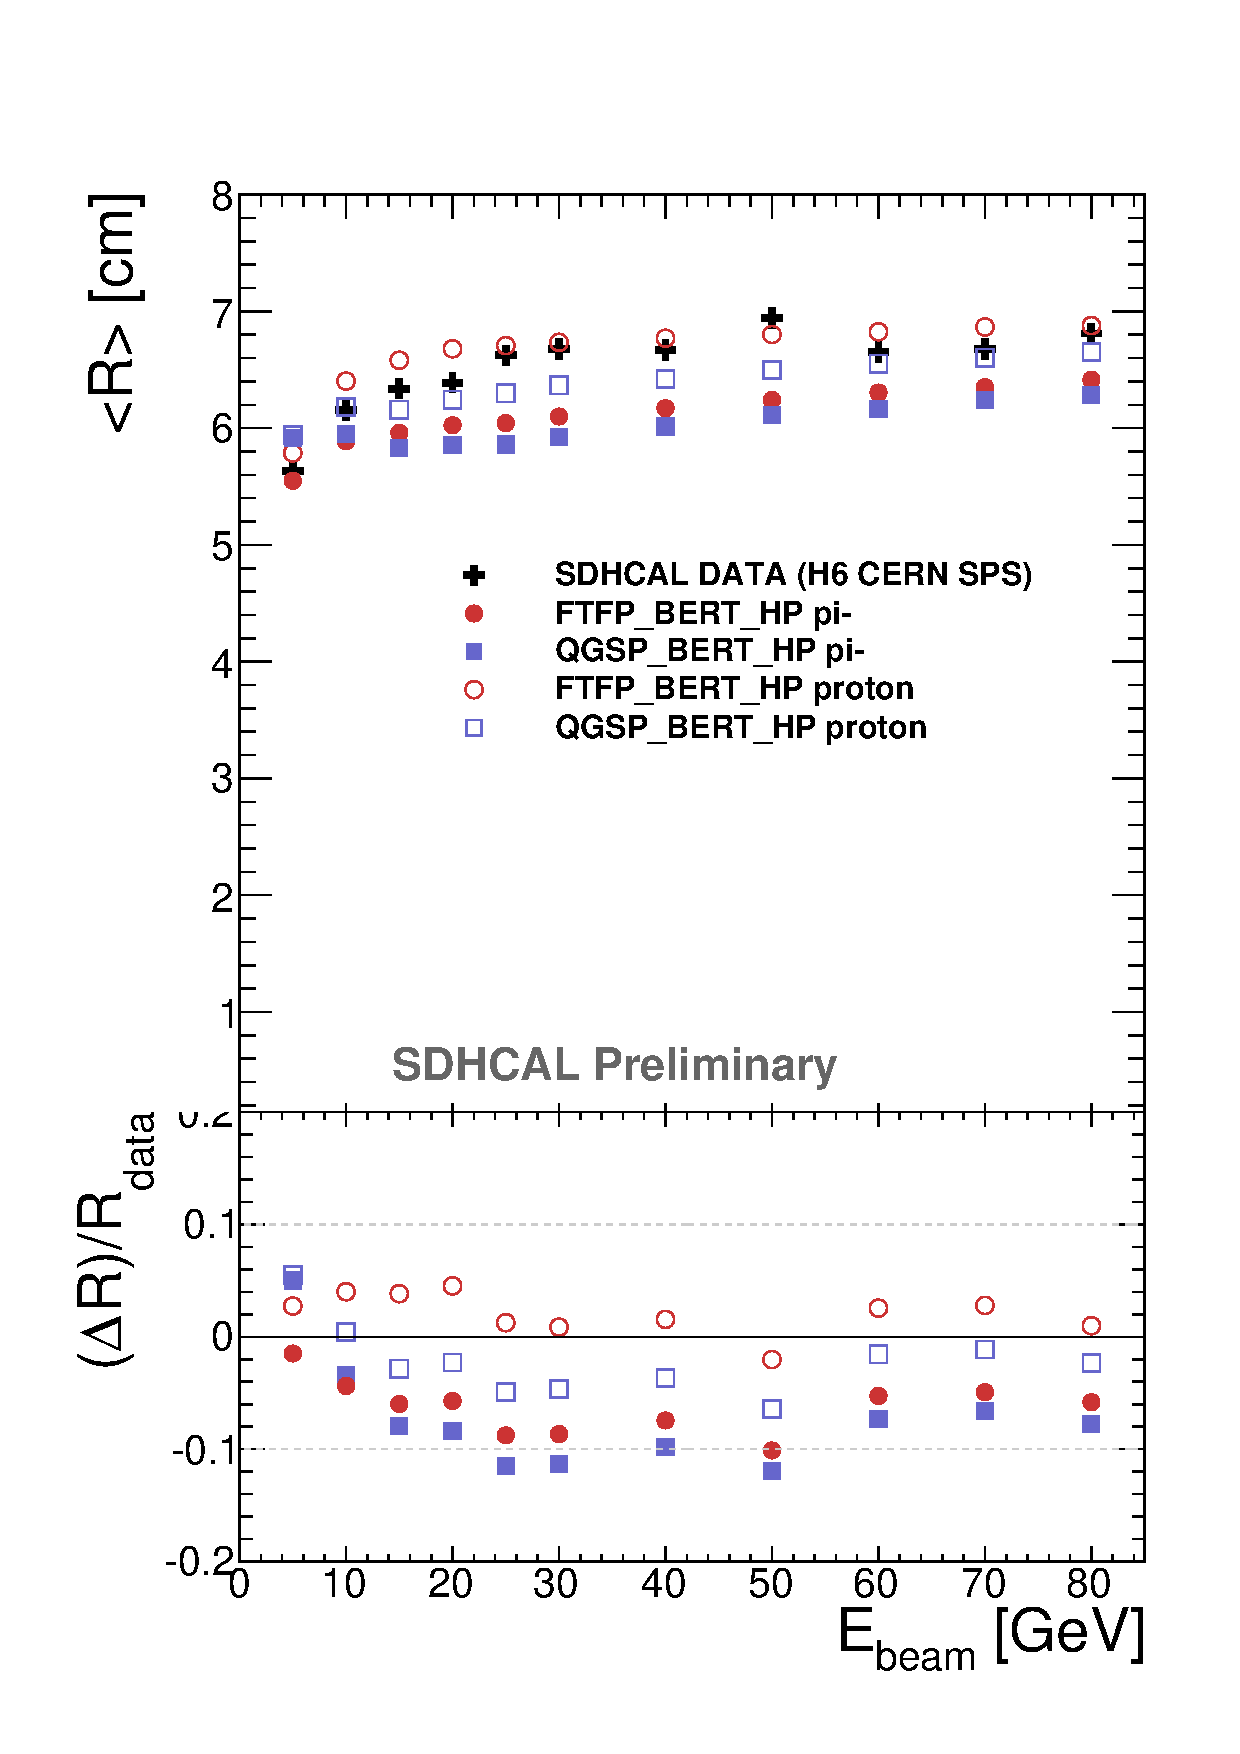
\includegraphics[width=0.49\linewidth]{figs/RADPIONHP.pdf}
      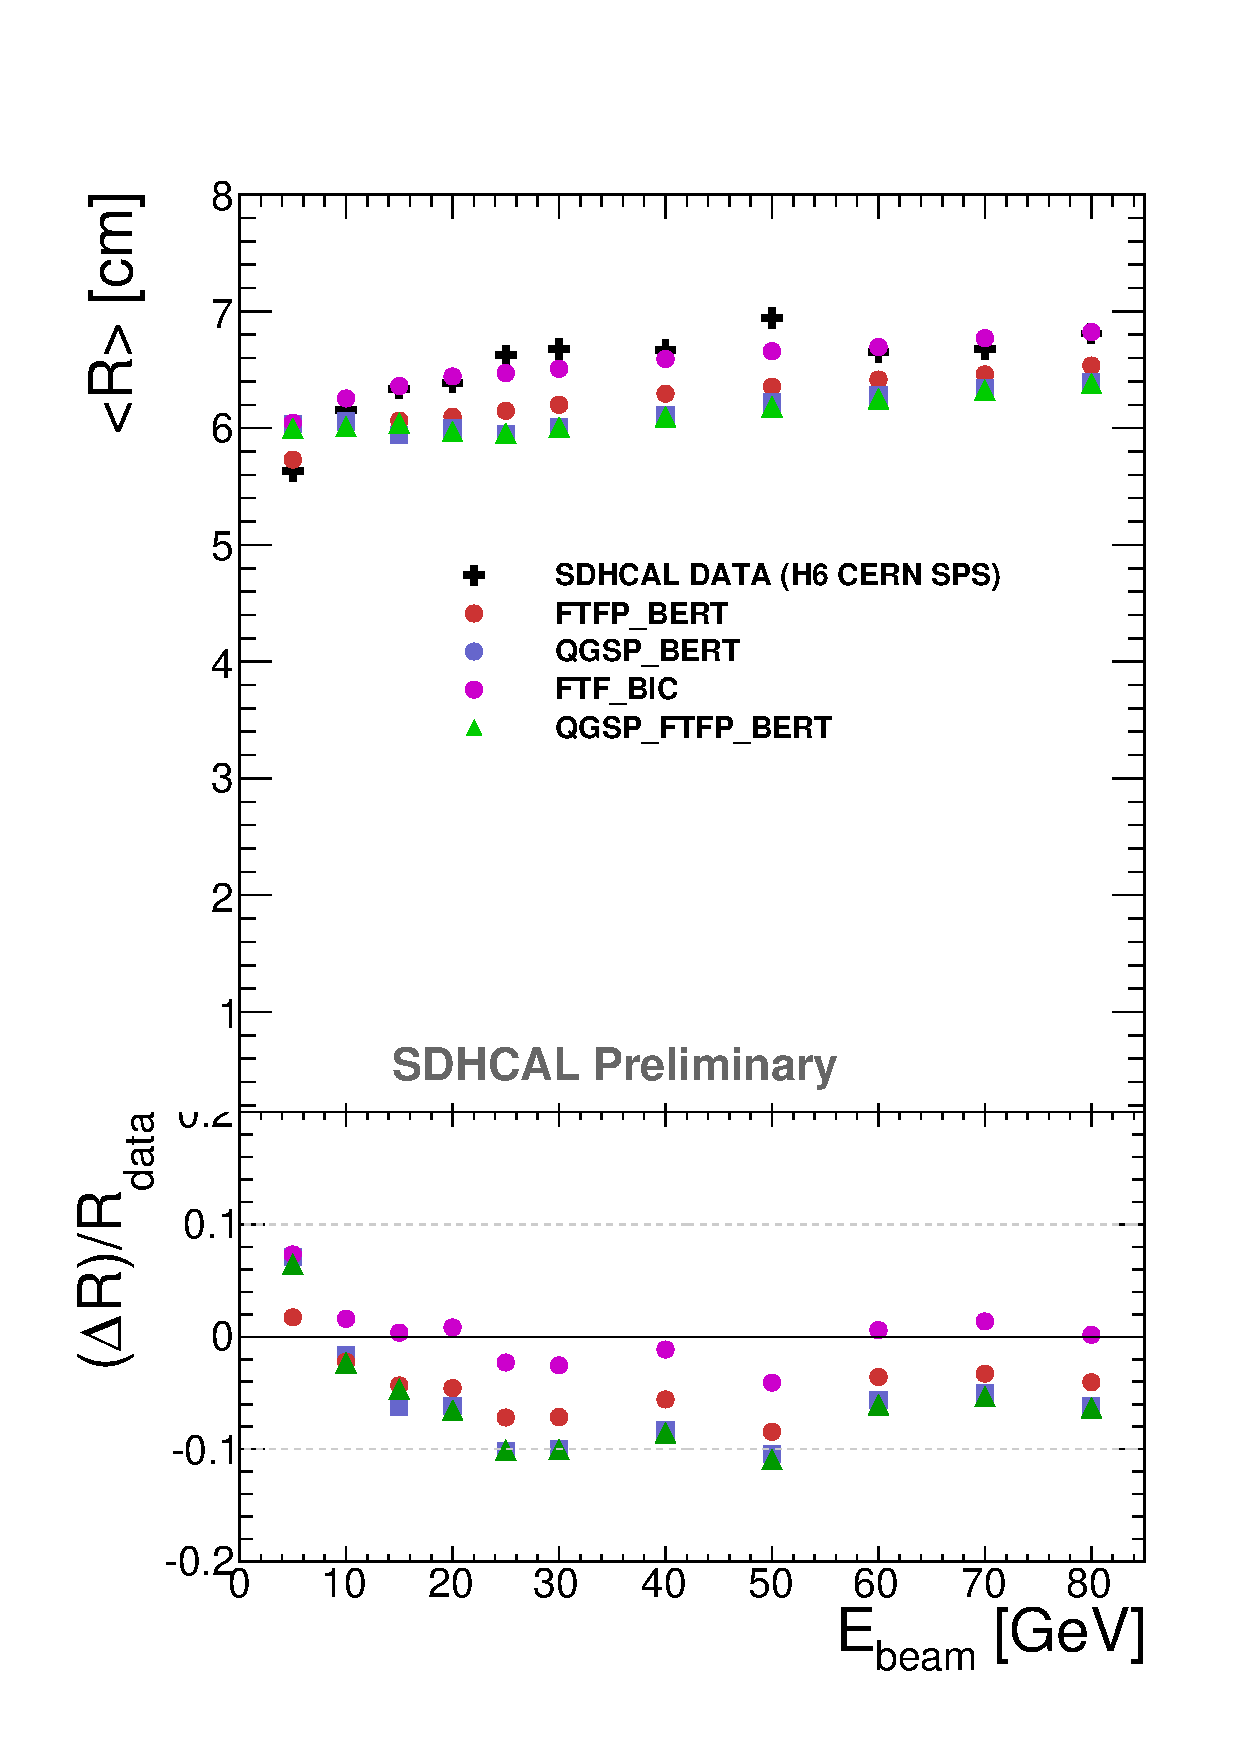
\includegraphics[width=0.49\linewidth]{figs/RADPROF_PION_MODEL.pdf}
    \end{center}
    \crefarticle{Thèse A. Steen}{2015LYO10230}
  \end{frame}




  %%%%%%%%%
  %% PFA %%
  %%%%%%%%%
  \section{Les algorithmes de suivi de particules}

  \begin{frame}
  \frametitle{\secname}
    \tableofcontents[currentsection]
  \end{frame}

  \subsection{Introduction}

  \begingroup
  \small
  \begin{frame}
  \frametitle{\secname}
  \framesubtitle{\subsecname}
    \begin{block}{Définition}
      \centering \textcolor{red}{Algorithme(s) de reconstruction} visant à reconstruire les particules \textcolor{blue}{individuellement} en \textcolor{red}{combinant les informations} les plus appropriées des \textcolor{blue}{différents sous-détecteurs}.
    \end{block}
    \pause
    \begin{center} \textbf{\large PFA = \textcolor{red}{Logiciel} + \textcolor{blue}{Détecteur} !} \end{center}
    \pause
    \begin{minipage}{0.48\linewidth}
      \begin{block}{Sous-détecteurs appropriés}
        \begin{itemize}
          \item $e^{\pm}$ : \textbf{Tracker}
          \item $h^{\pm}$ : \textbf{Tracker}
          \item $\mu^{\pm}$ : \textbf{Tracker} + chambres à muons
          \item $\gamma$ ~~~: \textbf{ECal} + Tracker (track veto)
          \item $h^{0}$ ~: \textbf{ECal + HCal}
        \end{itemize}
      \end{block}
      \begin{block}{Composition moyenne d'un jet de 100 GeV}
        \begin{itemize}
          \item 65 \% particules chargées
          \item 25 \% photons
          \item 10 \% hadrons neutres
        \end{itemize}
        \crefarticle{}{NIM \textbf{A495} (2002), 107–120}
      \end{block}
    \end{minipage} \hfill
    \begin{minipage}{0.5\linewidth}
      \begin{center}
        \includegraphics[width=0.95\linewidth]{pfa_event_display.png}
      \end{center}
    \end{minipage}
  \end{frame}
  \endgroup

  \begingroup
  \footnotesize
  \begin{frame}
  \frametitle{\secname}
  \framesubtitle{\subsecname - PandoraPFA}
    \begin{minipage}{0.6\linewidth}
    \begin{block}{PandoraPFA}
      \begin{enumerate}
        \item<2-> \textcolor{red}{\textit{Clustering} en cône récursifs}
        \item<3-> \textcolor{MyGreen}{Associations topologiques}
        \begin{itemize}
          \item<3-> \textcolor{MyGreen}{\footnotesize Association trace $\leftrightarrow$ cluster}
          \item<3-> \textcolor{MyGreen}{\footnotesize Association cluster $\leftrightarrow$ cluster}
        \end{itemize}
        \item<4->  \textbf{\textit{Re-clustering} statistique}
        \begin{itemize}
          \item<4-> \textbf{\footnotesize Compatibilité $E-p$}
          \item<4-> \textbf{\footnotesize Clustering local}
        \end{itemize}
        \item<5-> \textcolor{blue}{Suppression des fragments}
      \end{enumerate}
    \end{block}
    ~
    \end{minipage} \hfill
    \begin{minipage}{0.39\linewidth}
      \begin{center}
        \begin{tikzpicture}
          \node<2->[anchor=south west,inner sep=0] at (0,0) {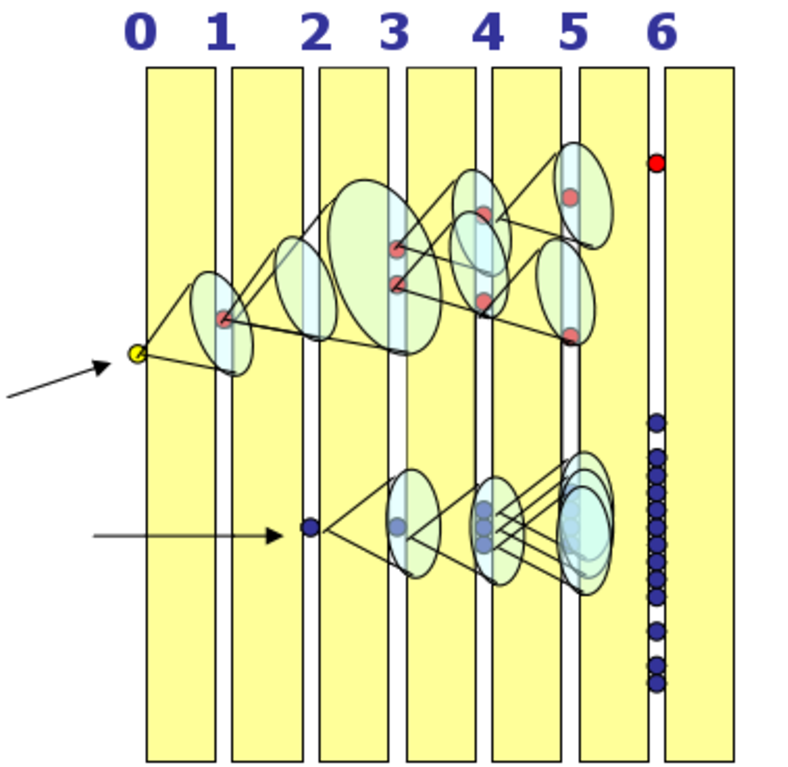
\includegraphics[width=0.9\linewidth]{figs/ConeAlgorithm.pdf}};
          \draw<2->[red,  thick, overlay] (0,-0.1) rectangle (3.8,3.8);
        \end{tikzpicture}
      \end{center}
    \end{minipage}

    \begin{minipage}{0.6\linewidth}
      \vspace{-7pt}
      \begin{center}
        {\onslide<3-> 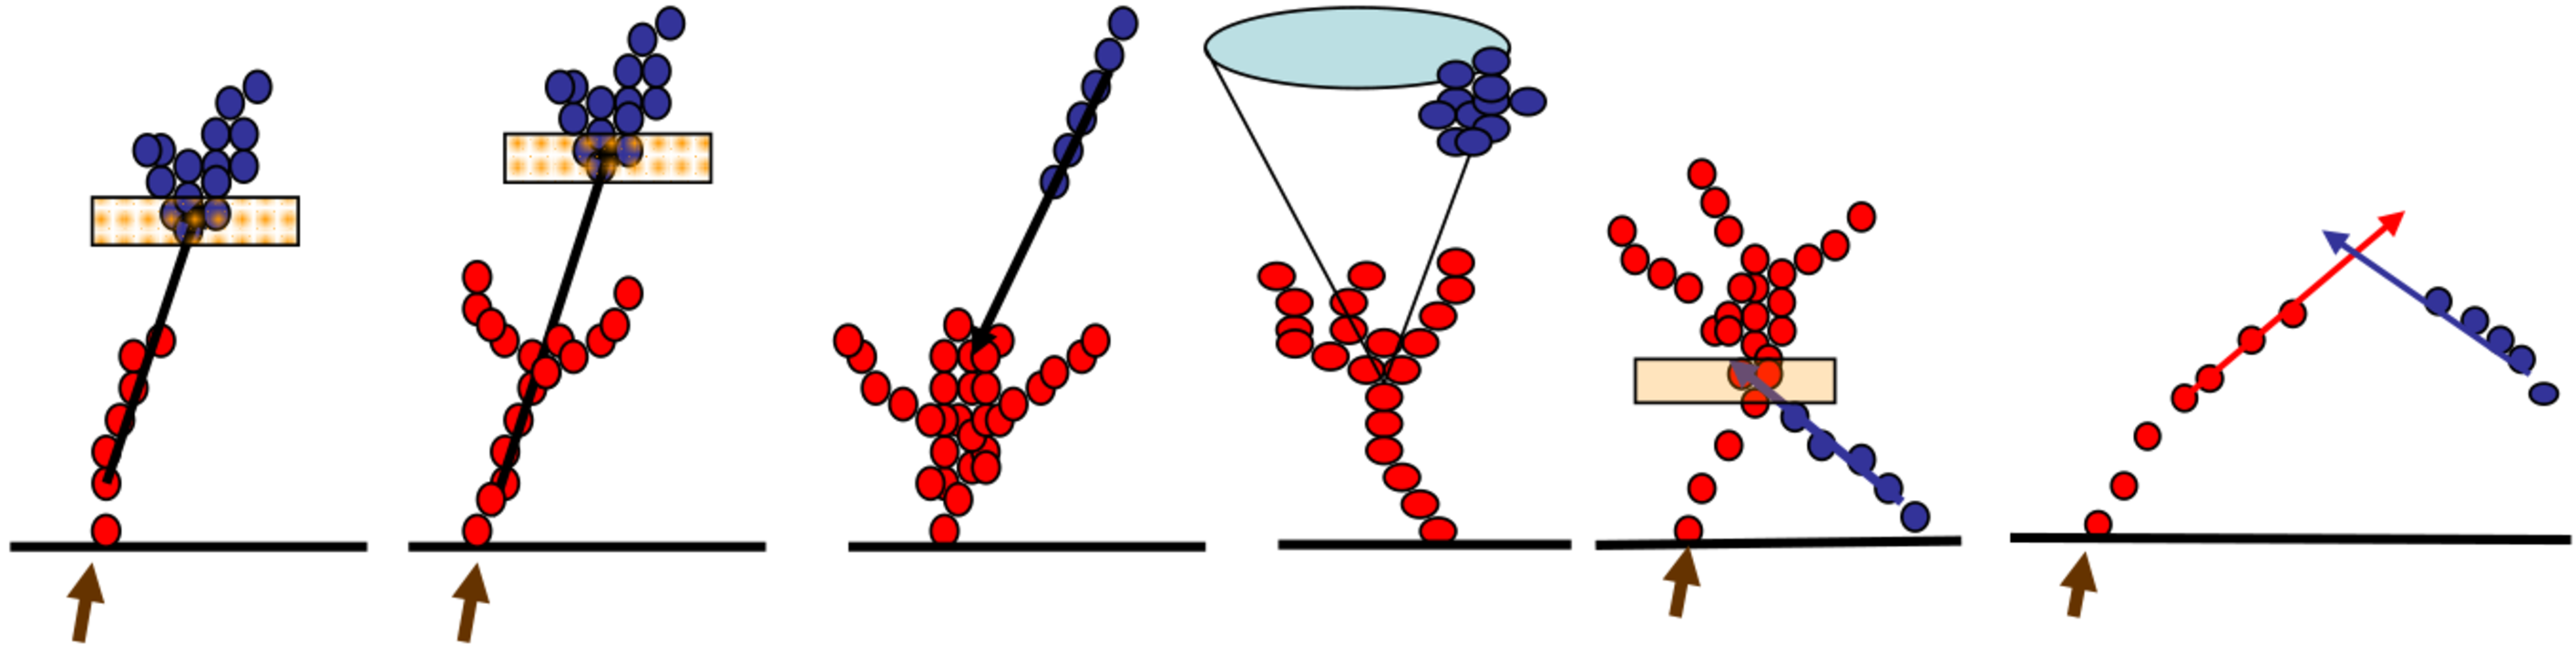
\includegraphics[width=\linewidth]{PandoraAssociations.pdf}
        \begin{tikzpicture}
          \draw[MyGreen,  thick, overlay] (0.1,-0) rectangle (-6.55,1.65);
        \end{tikzpicture}} \\
        \vspace{0.1cm}
        {\onslide<5-> 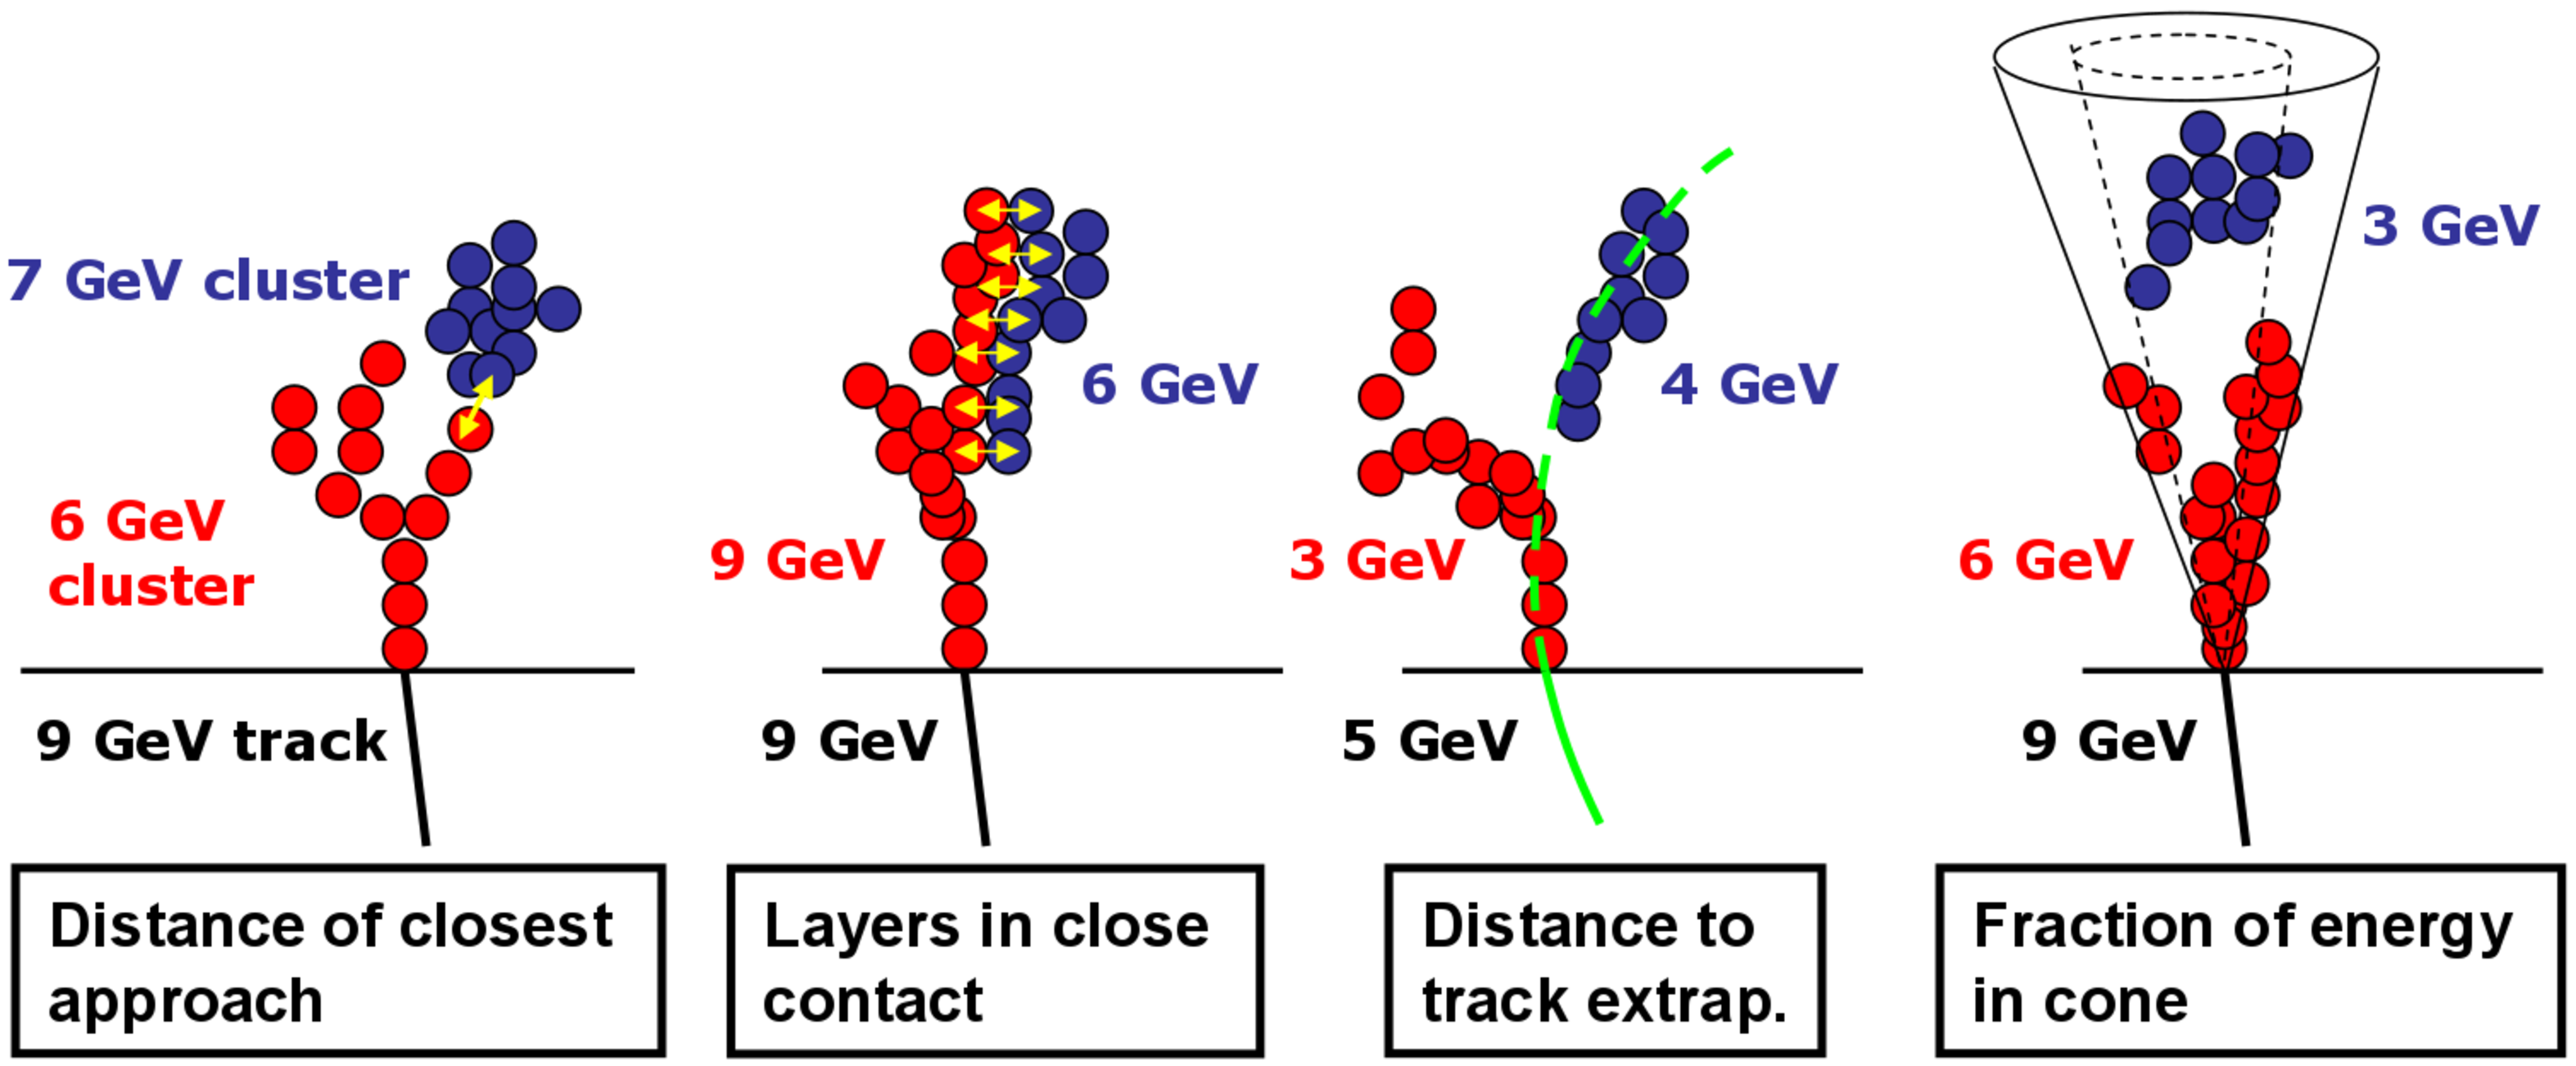
\includegraphics[width=0.8\linewidth]{PandoraFragmentRemoval.pdf}
        \begin{tikzpicture}
          \draw[blue,  thick, overlay] (0.1,-0.1) rectangle (-5.3,2.15);
        \end{tikzpicture}}
      \end{center}
    \end{minipage} ~ \hfill
    \begin{minipage}{0.37\linewidth}
      \begin{center}
        {\onslide<4-> 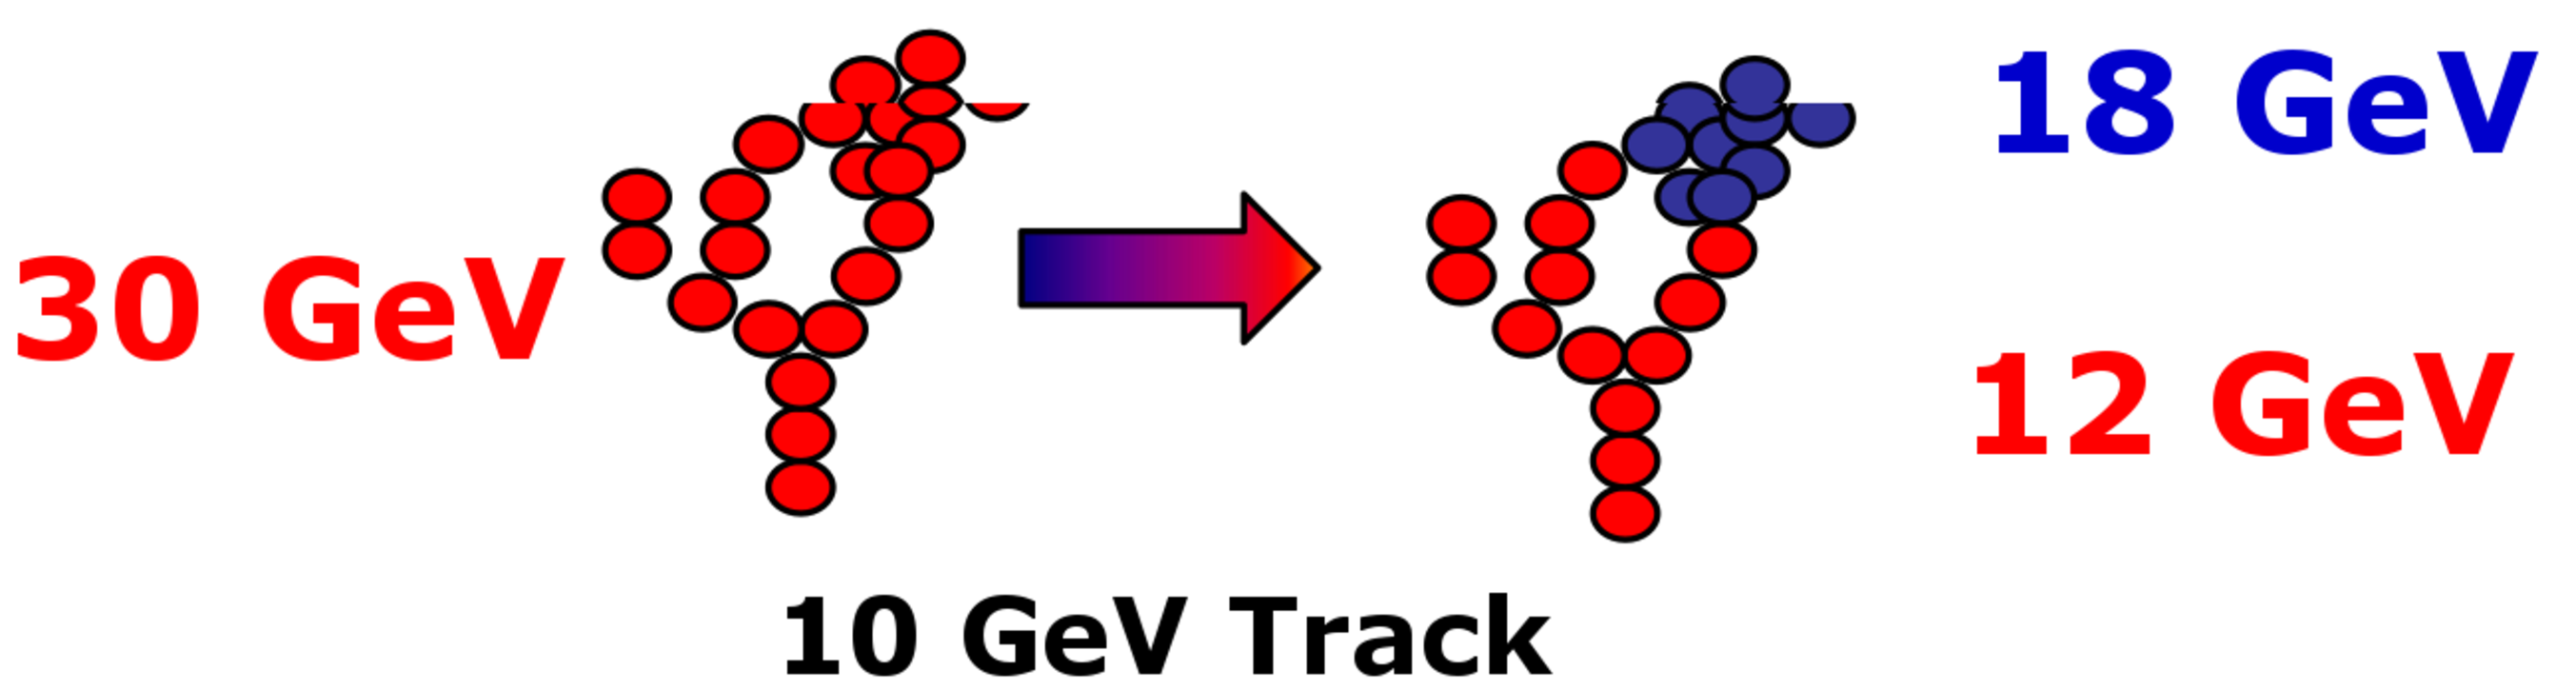
\includegraphics[width=\linewidth]{PandoraReclustering-ClusterSplitting.pdf} \\ ~ \\
        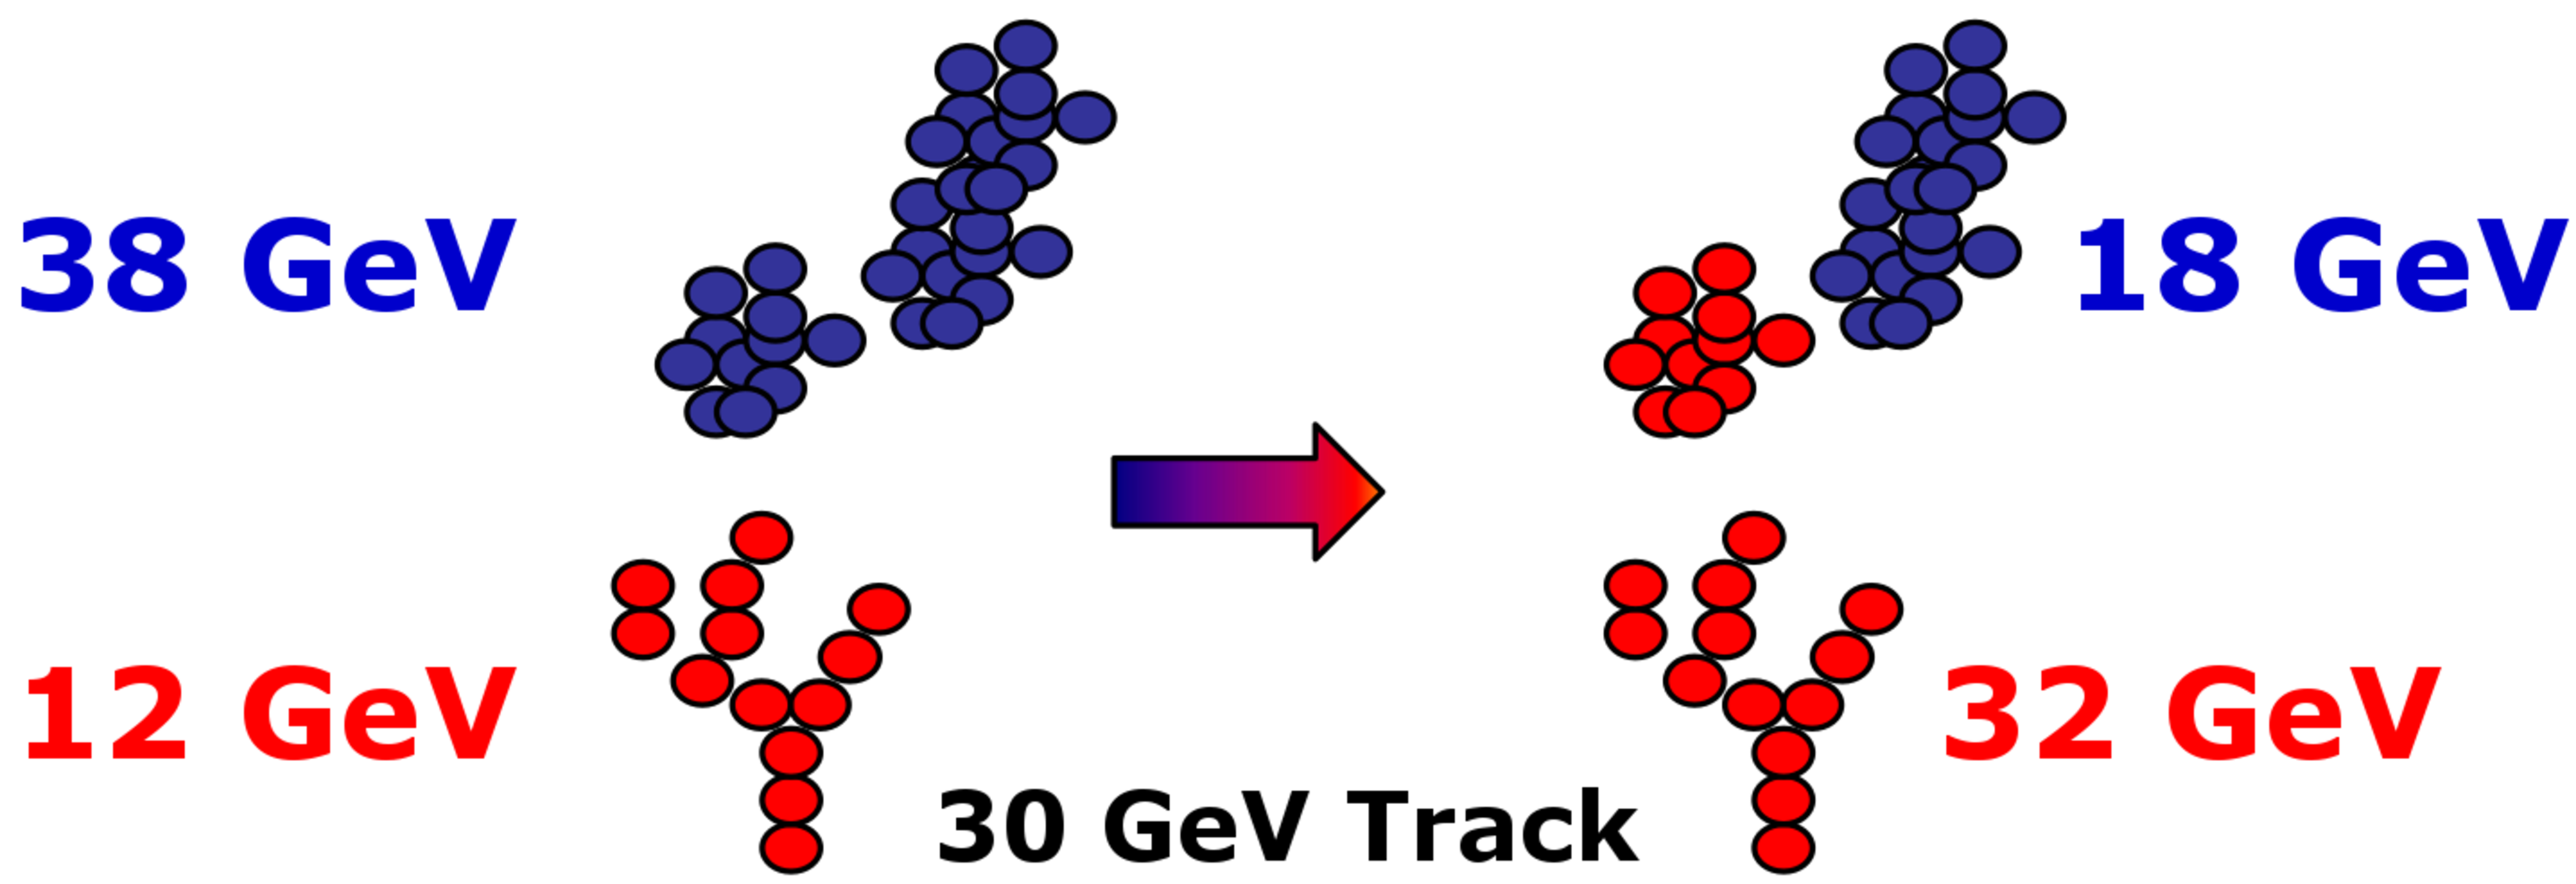
\includegraphics[width=\linewidth]{PandoraReclustering-MergeSplit.pdf}
        \begin{tikzpicture}
          \draw[black,  thick, overlay] (0.1,-0.1) rectangle (-4.1,2.9);
        \end{tikzpicture}}
      \end{center}
    \end{minipage}
  \end{frame}
  \endgroup

  \begin{frame}
  \frametitle{\secname}
  \framesubtitle{\subsecname - les performances de PandoraPFA}

  \begin{minipage}{0.6\linewidth}

    \begin{block}{Extraction des performances}
      \begin{itemize}
        \item Boson $Z^0$ virtuel $\rightarrow$ \textit{jj}
        \item Énergies : 91, 200, 360 et 500 $GeV$
      \end{itemize}
    \end{block}

    {\onslide<2->
    \begin{block}{Les limites de PandoraPFA}
      \begin{itemize}
        \item Conçu pour un HCal analogique
        \item Optimisé pour une taille de cellule 3x3$cm^2$
        \item Calcul d'énergie linéaire dans les algorithmes
      \end{itemize}
    \end{block}

    \begin{center}
      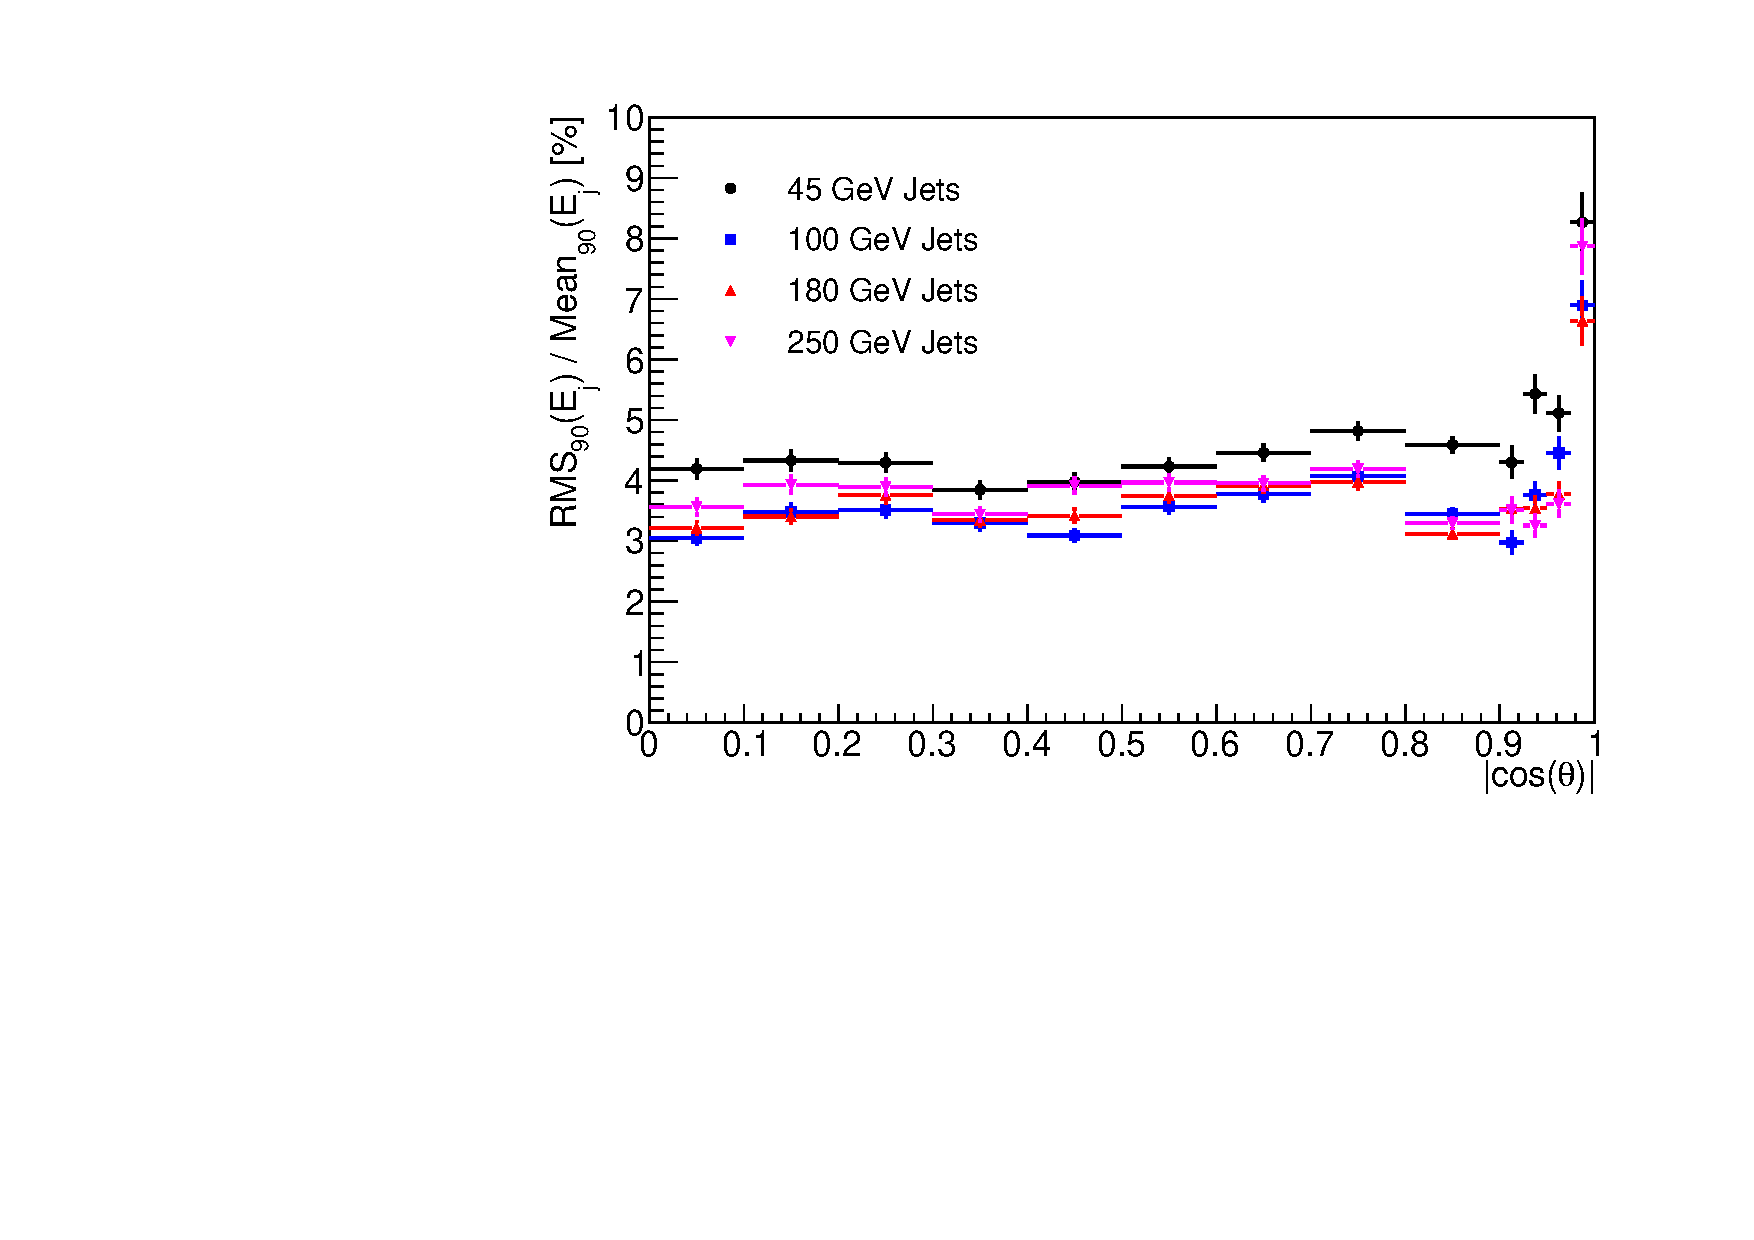
\includegraphics[width=0.7\linewidth]{PandoraPFA_JER_ILD_v05_o2.pdf}
    \end{center}
    \crefarticle{Thèse A. Steen}{2015LYO10230}
    }

  \end{minipage} ~~ \hfill
  \begin{minipage}{0.37\linewidth}

    \begin{center}
      {\onslide<1-> 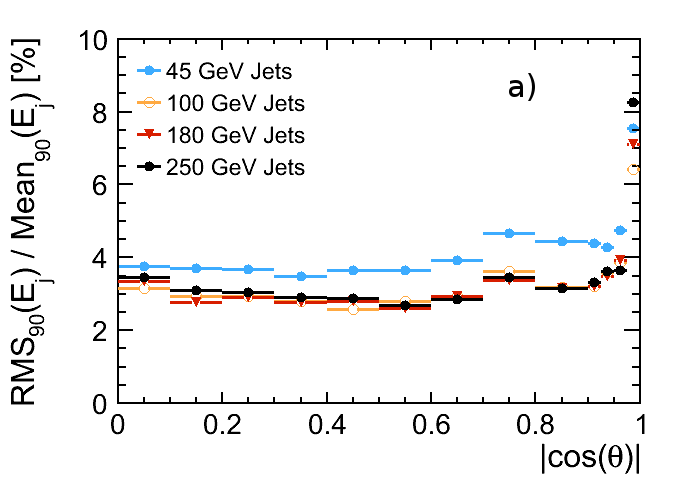
\includegraphics[width=1.07\linewidth]{PandoraPFA_JER_ILD_v05_o1.png} \\
      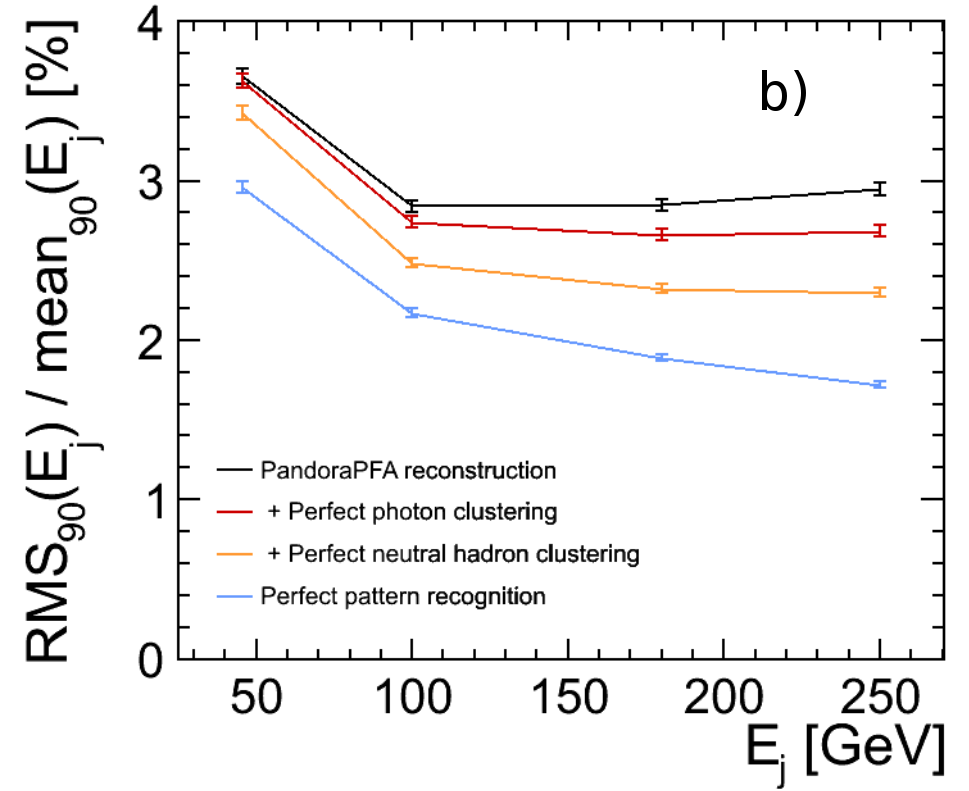
\includegraphics[width=\linewidth]{PandoraPFA_JER_ILD_v05_o1_Cheating.png}
      \crefarticle{M. A. Thomson\\}{\textbf{NIM}, A611:25-40,2009}
      }
    \end{center}

  \end{minipage}

  \end{frame}

  \subsection{Principe d'ArborPFA}
  \begin{frame}
  \frametitle{\secname}
  \framesubtitle{\subsecname}
  \begin{block}{Principe}
    \begin{center}Algorithme de \textit{clustering} basé sur la \textbf{topologie en arbre} des gerbes hadroniques.\end{center}
  \end{block}
  \pause
  \begin{minipage}{0.325\linewidth}
    \begin{center}
      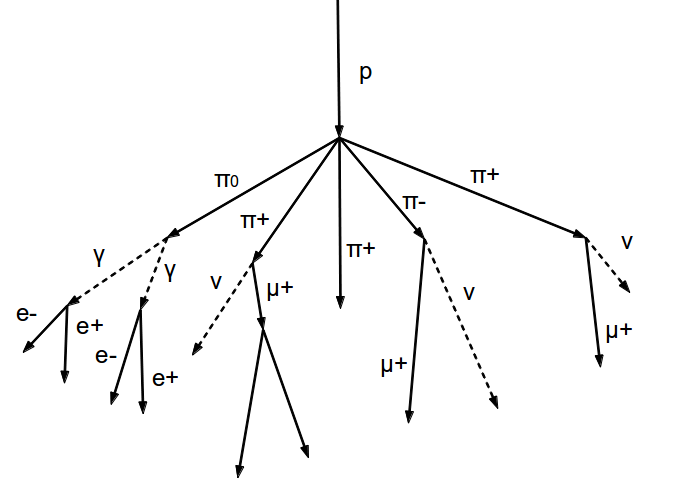
\includegraphics[width=\linewidth]{ProtonDecay.png} \\
      Gerbe hadronique
    \end{center}
  \end{minipage} \hfill
  \begin{minipage}{0.325\linewidth}
    \begin{center}
      \pause
      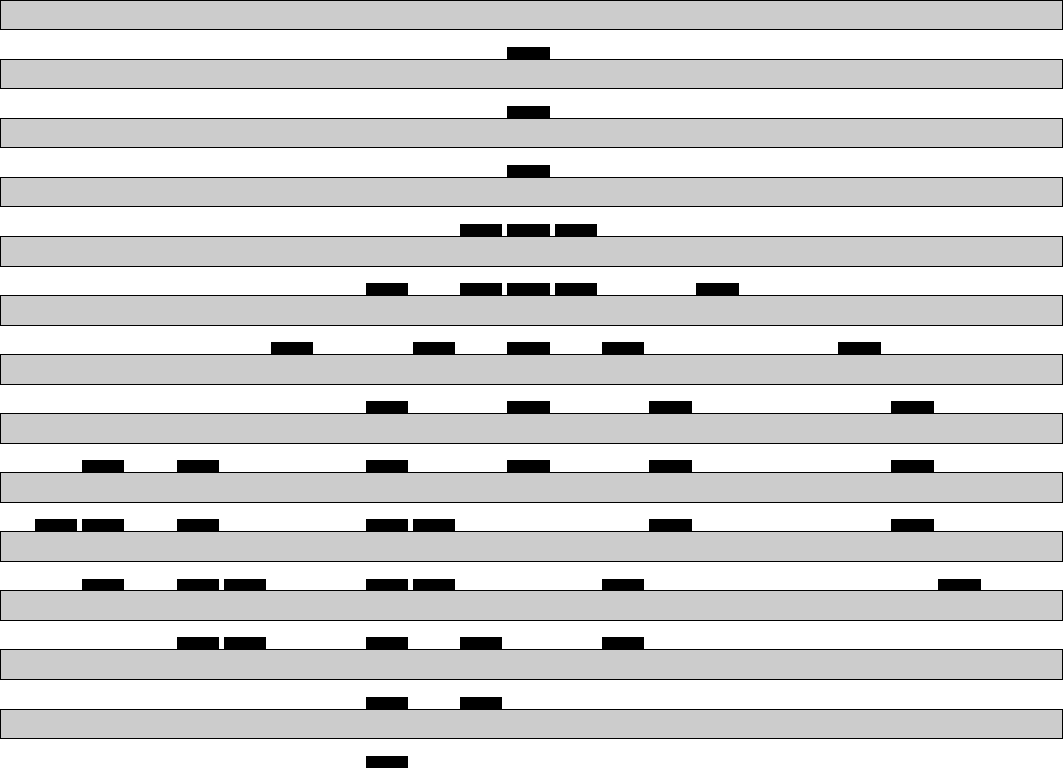
\includegraphics[width=\linewidth]{ProtonDecayCaloNoConnector.pdf} \\
      dans un calorimètre
    \end{center}
  \end{minipage}\hfill
  \begin{minipage}{0.325\linewidth}
    \begin{center}
      \pause
      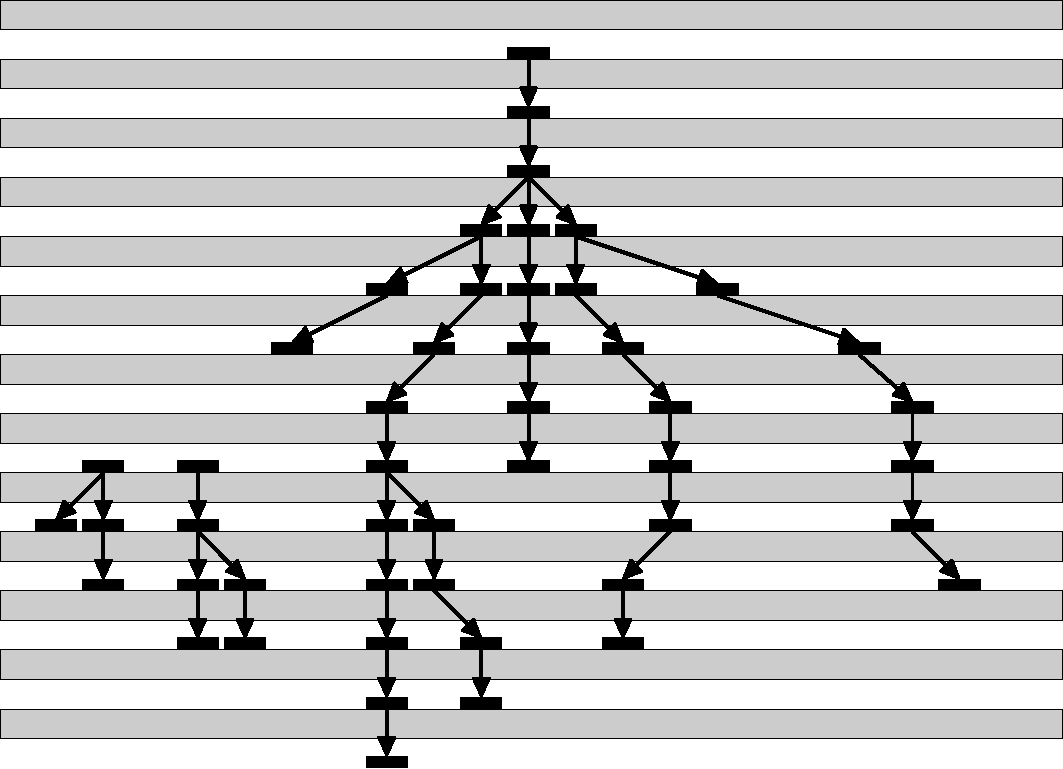
\includegraphics[width=\linewidth]{ProtonDecayCalo.pdf} \\
      avec ArborPFA
    \end{center}
  \end{minipage}
  \pause
  \begin{block}{Quelques définitions}
    \begin{itemize}
      \item \textbf{Vertex} : \textit{Point} (\textit{sommet}) dans l'espace relié par un ou plusieurs connecteurs (+ vertex racines et feuilles)
      \item \textbf{Connecteur} : \textit{Lien} (\textit{arrête}) orienté liant deux vertex
      \item \textbf{Arbre} : Ensemble de vertex reliés par des connecteurs (\textit{arbre enraciné}).
      \begin{itemize}
        \item il est connexe
        \item possède un unique vertex sans prédecesseur,
        \item tous les autres vertex possèdent un unique prédécesseur.
      \end{itemize}
    \end{itemize}
  \end{block}
  \end{frame}


  \subsection{ArborPFA pour le SDHCAL}

  %% SDHCAL ArborPFA (1)
  \begin{frame}
  \frametitle{\secname}
  \framesubtitle{\subsecname}

    \begin{block}{ArborPFA pour le SDHCAL}
      \begin{itemize}
        \item Test du principe de l'algorithme
        \item Habilité à reconstruire une particule isolée
        \item Habilité à séparer un hadron neutre d'un chargé
      \end{itemize}
    \end{block}

    \pause
    \begin{minipage}{0.6\linewidth}
      \begin{block}{Implémentation}
        \begin{itemize}
          \item \textcolor<2>{red}{Création de vertex (1 algo)}
          \item \textcolor<3,7>{red}{Construction des arbres et clusters (6 algos)}
          \begin{itemize}
            \item \textcolor<3,7>{red}{Connexions des vertex (3 algos)}
            \item \textcolor<3,7>{red}{Nettoyage des connexions (3 algos)}
          \end{itemize}
          %\item \textcolor<2->{blue}{Association traces $\rightarrow$ clusters (1 algo)}
          \item \textcolor<4>{red}{Association traces $\rightarrow$ clusters (1 algo)}
          % \item \textcolor<2->{blue}{Association clusters $\rightarrow$ clusters (3 algos)}
          \item \textcolor<5>{red}{Association clusters $\rightarrow$ clusters (3 algos)}
          \item \textcolor<6>{red}{Création de PFOs (1 algo)}
        \end{itemize}
      \end{block}
    \end{minipage}
    \begin{minipage}{0.39\linewidth}
      \begin{overprint}
        \onslide<2> \centering 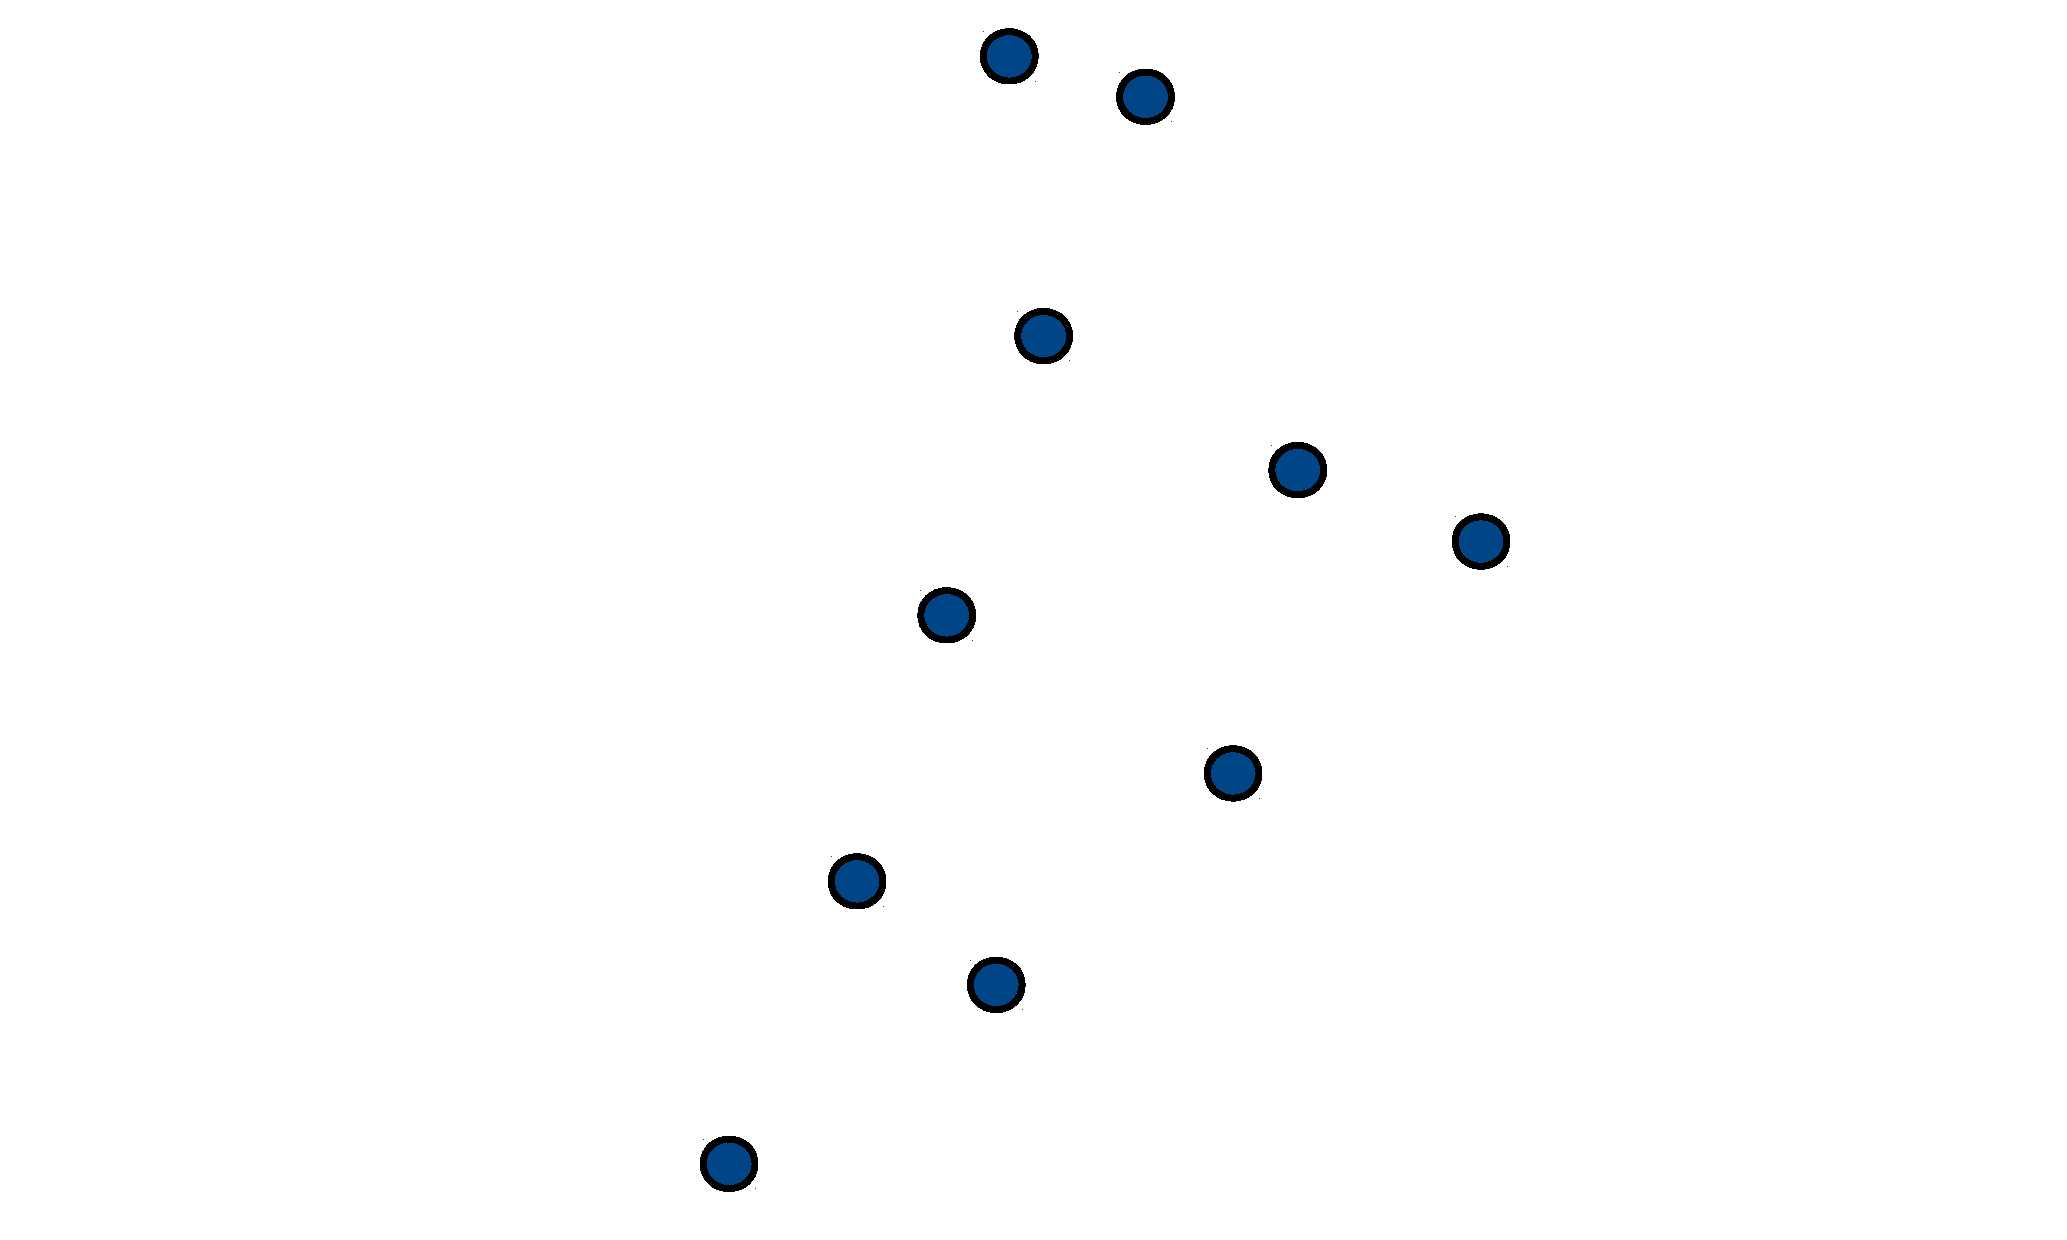
\includegraphics[width=0.8\linewidth]{VertexCreationIntro.pdf}
        \onslide<3,7> \centering 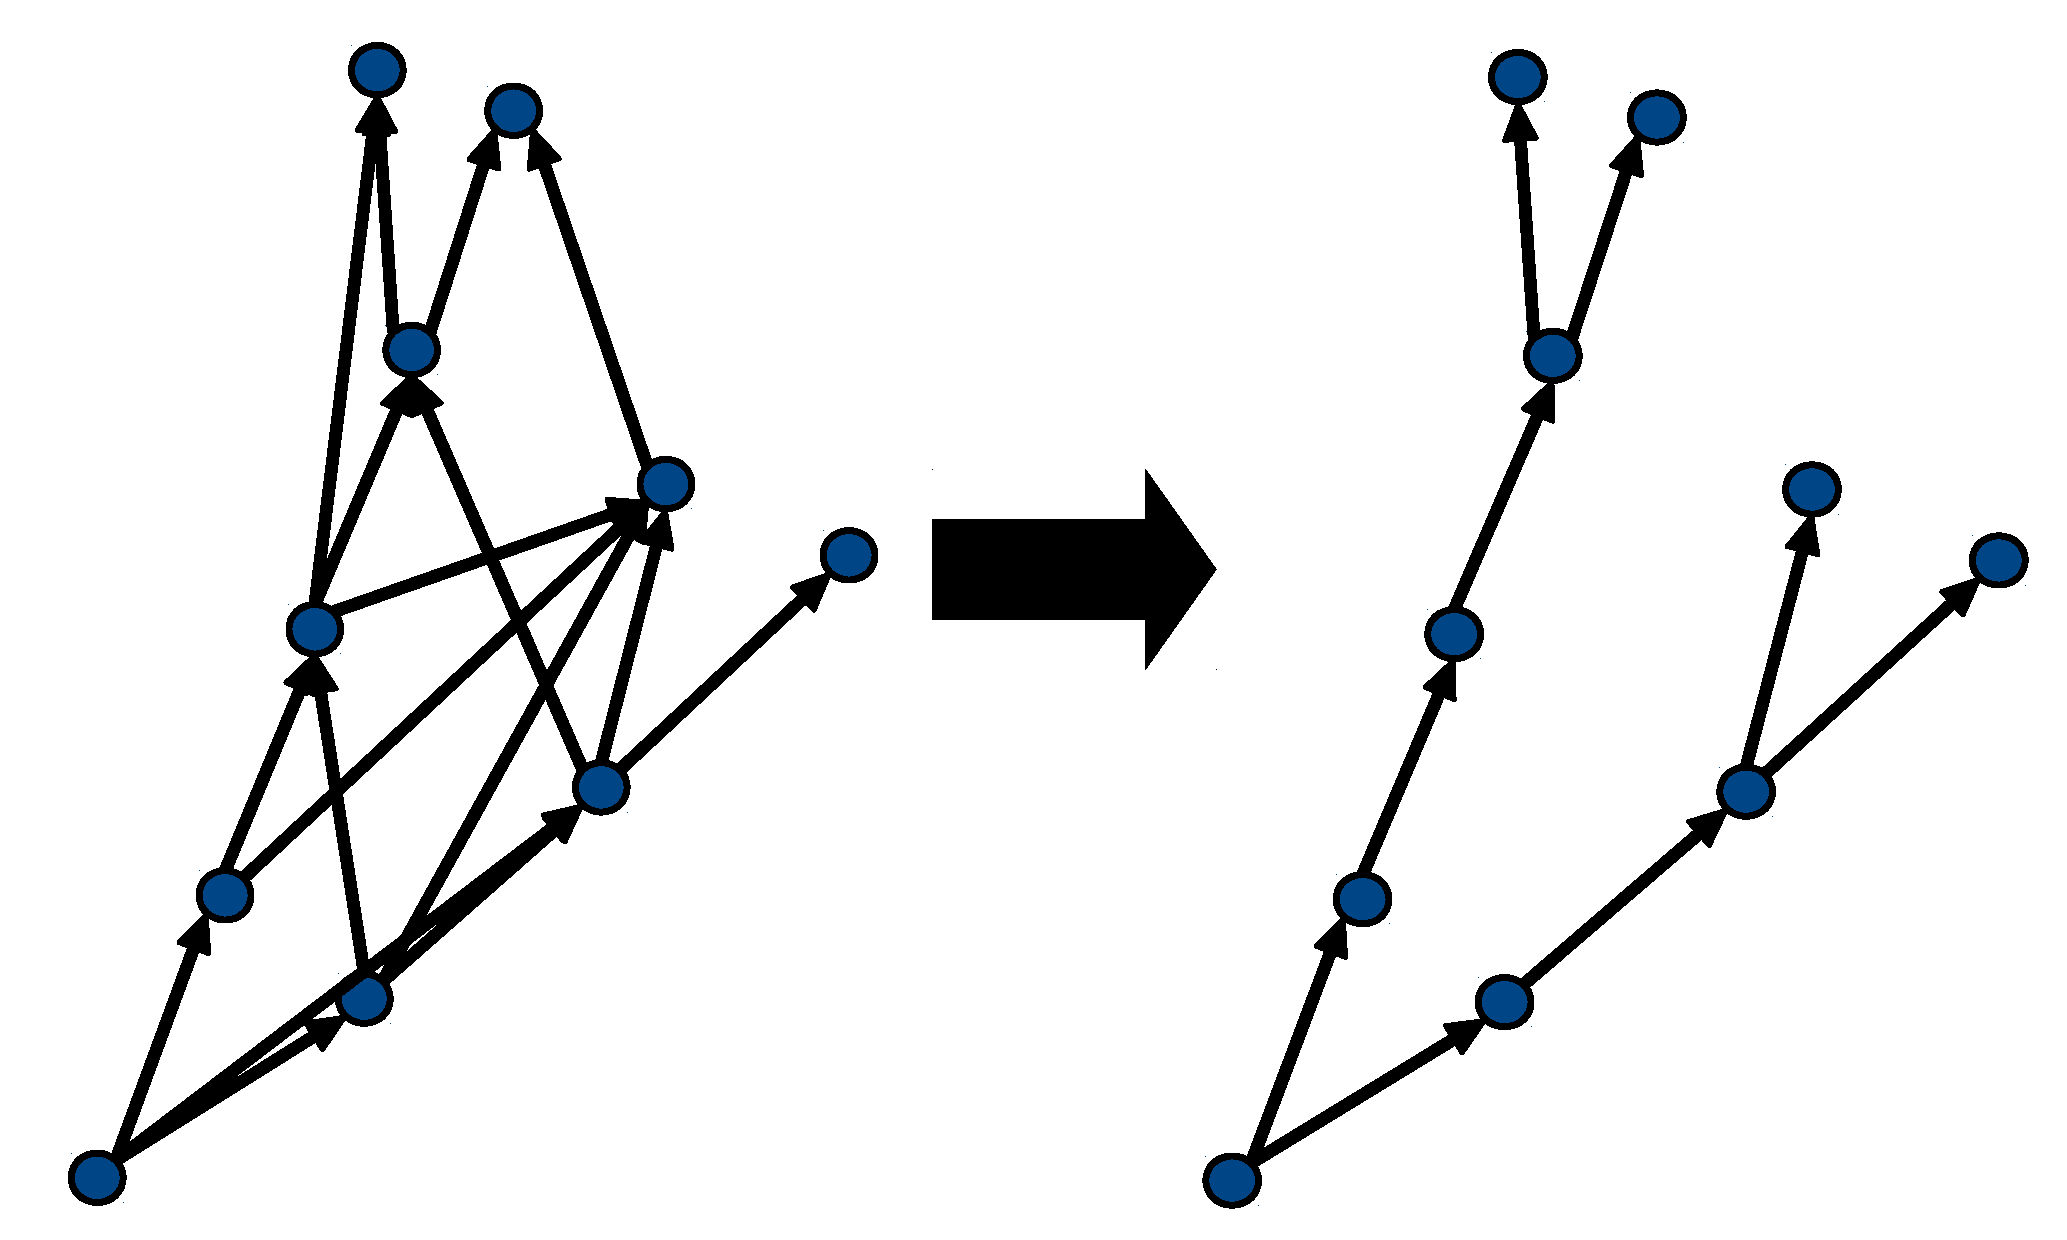
\includegraphics[width=0.8\linewidth]{ConnectCleanIntro.pdf}
        \onslide<4> \centering 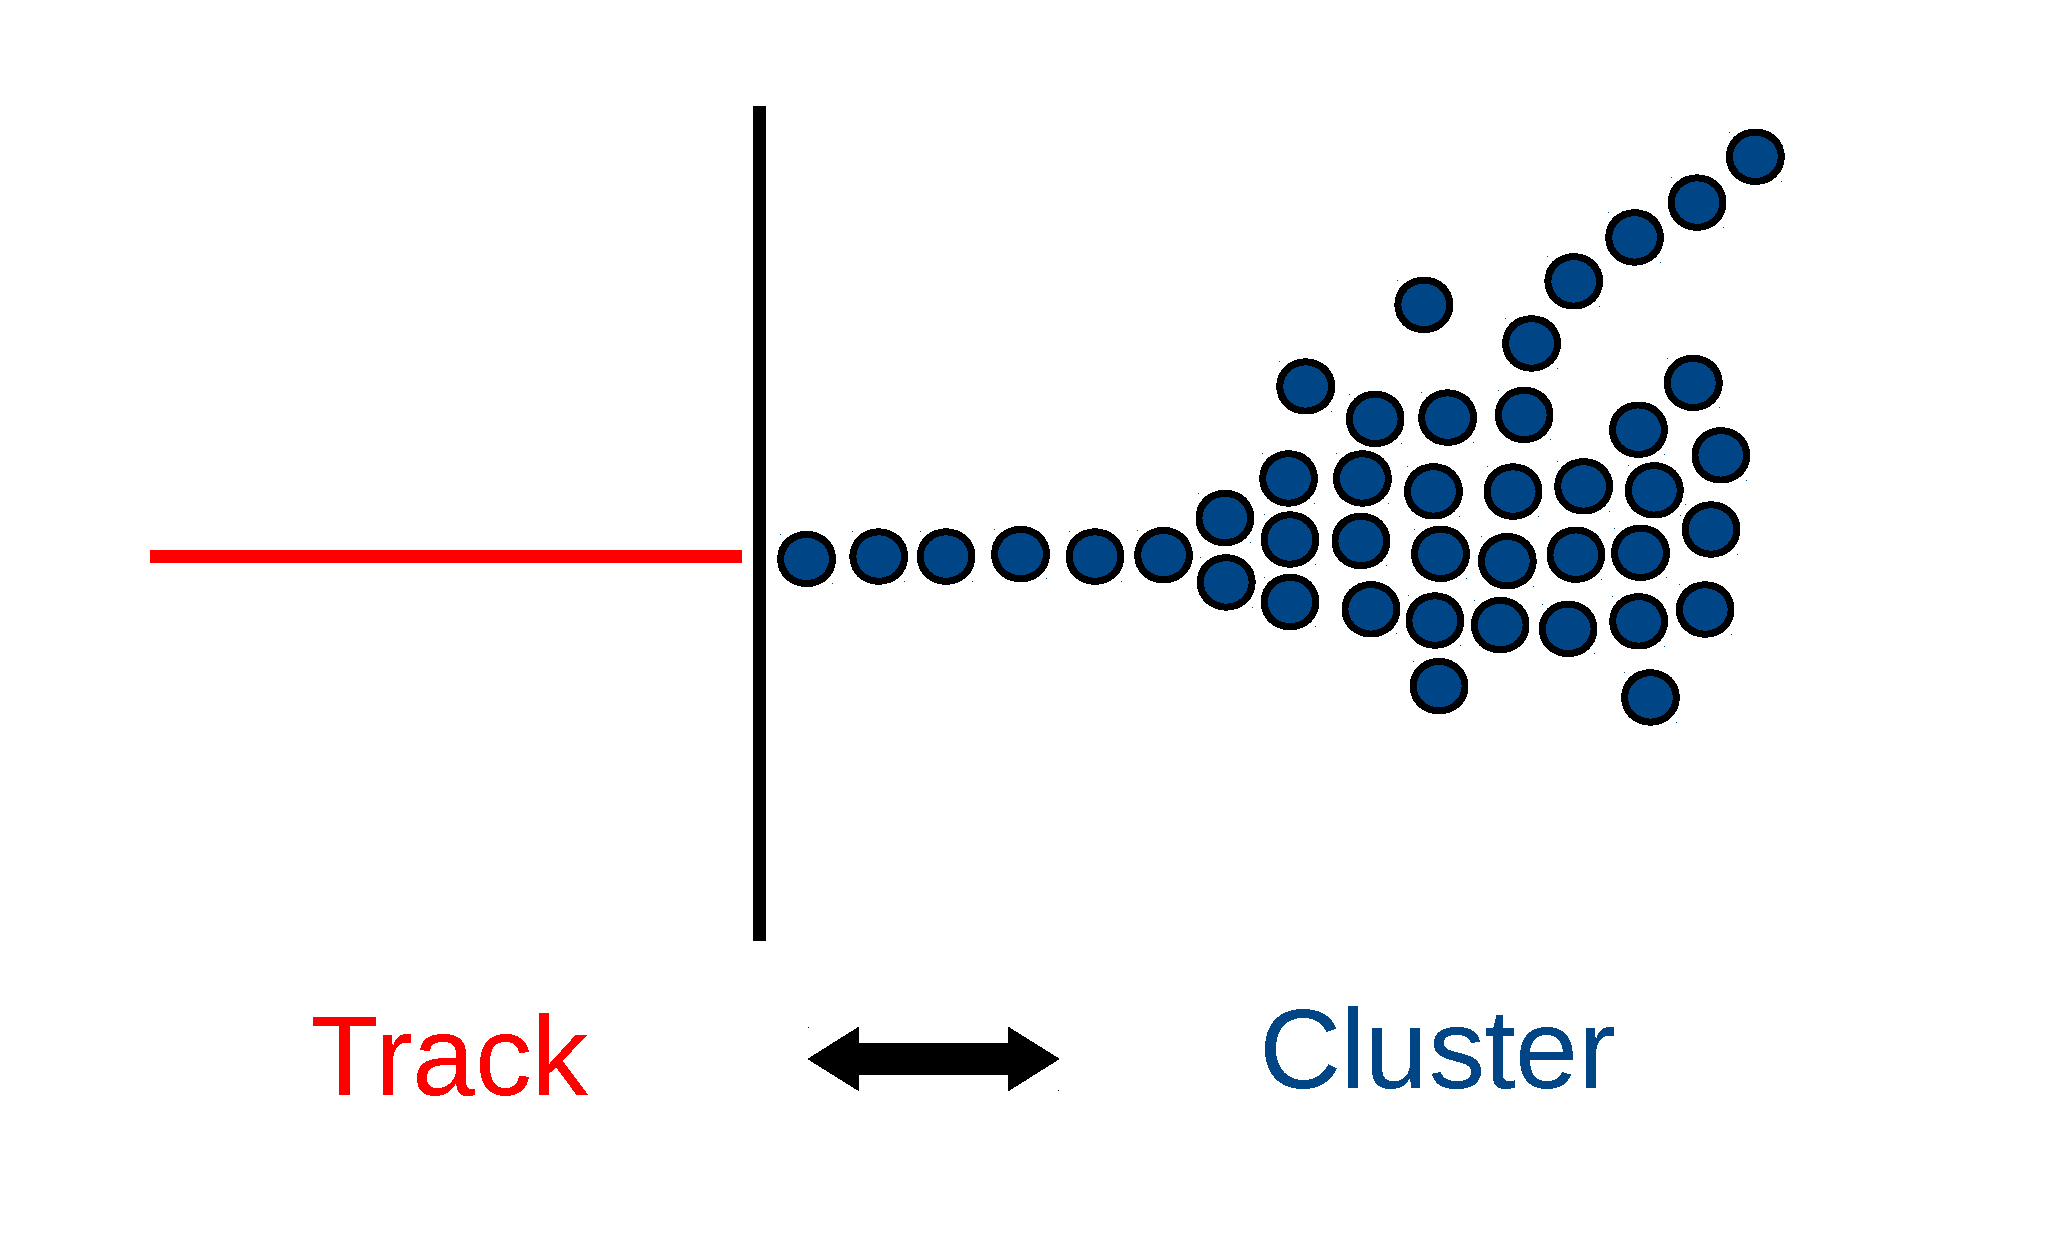
\includegraphics[width=0.8\linewidth]{TrackClusterAssociationIntro.pdf}
        \onslide<5> \centering 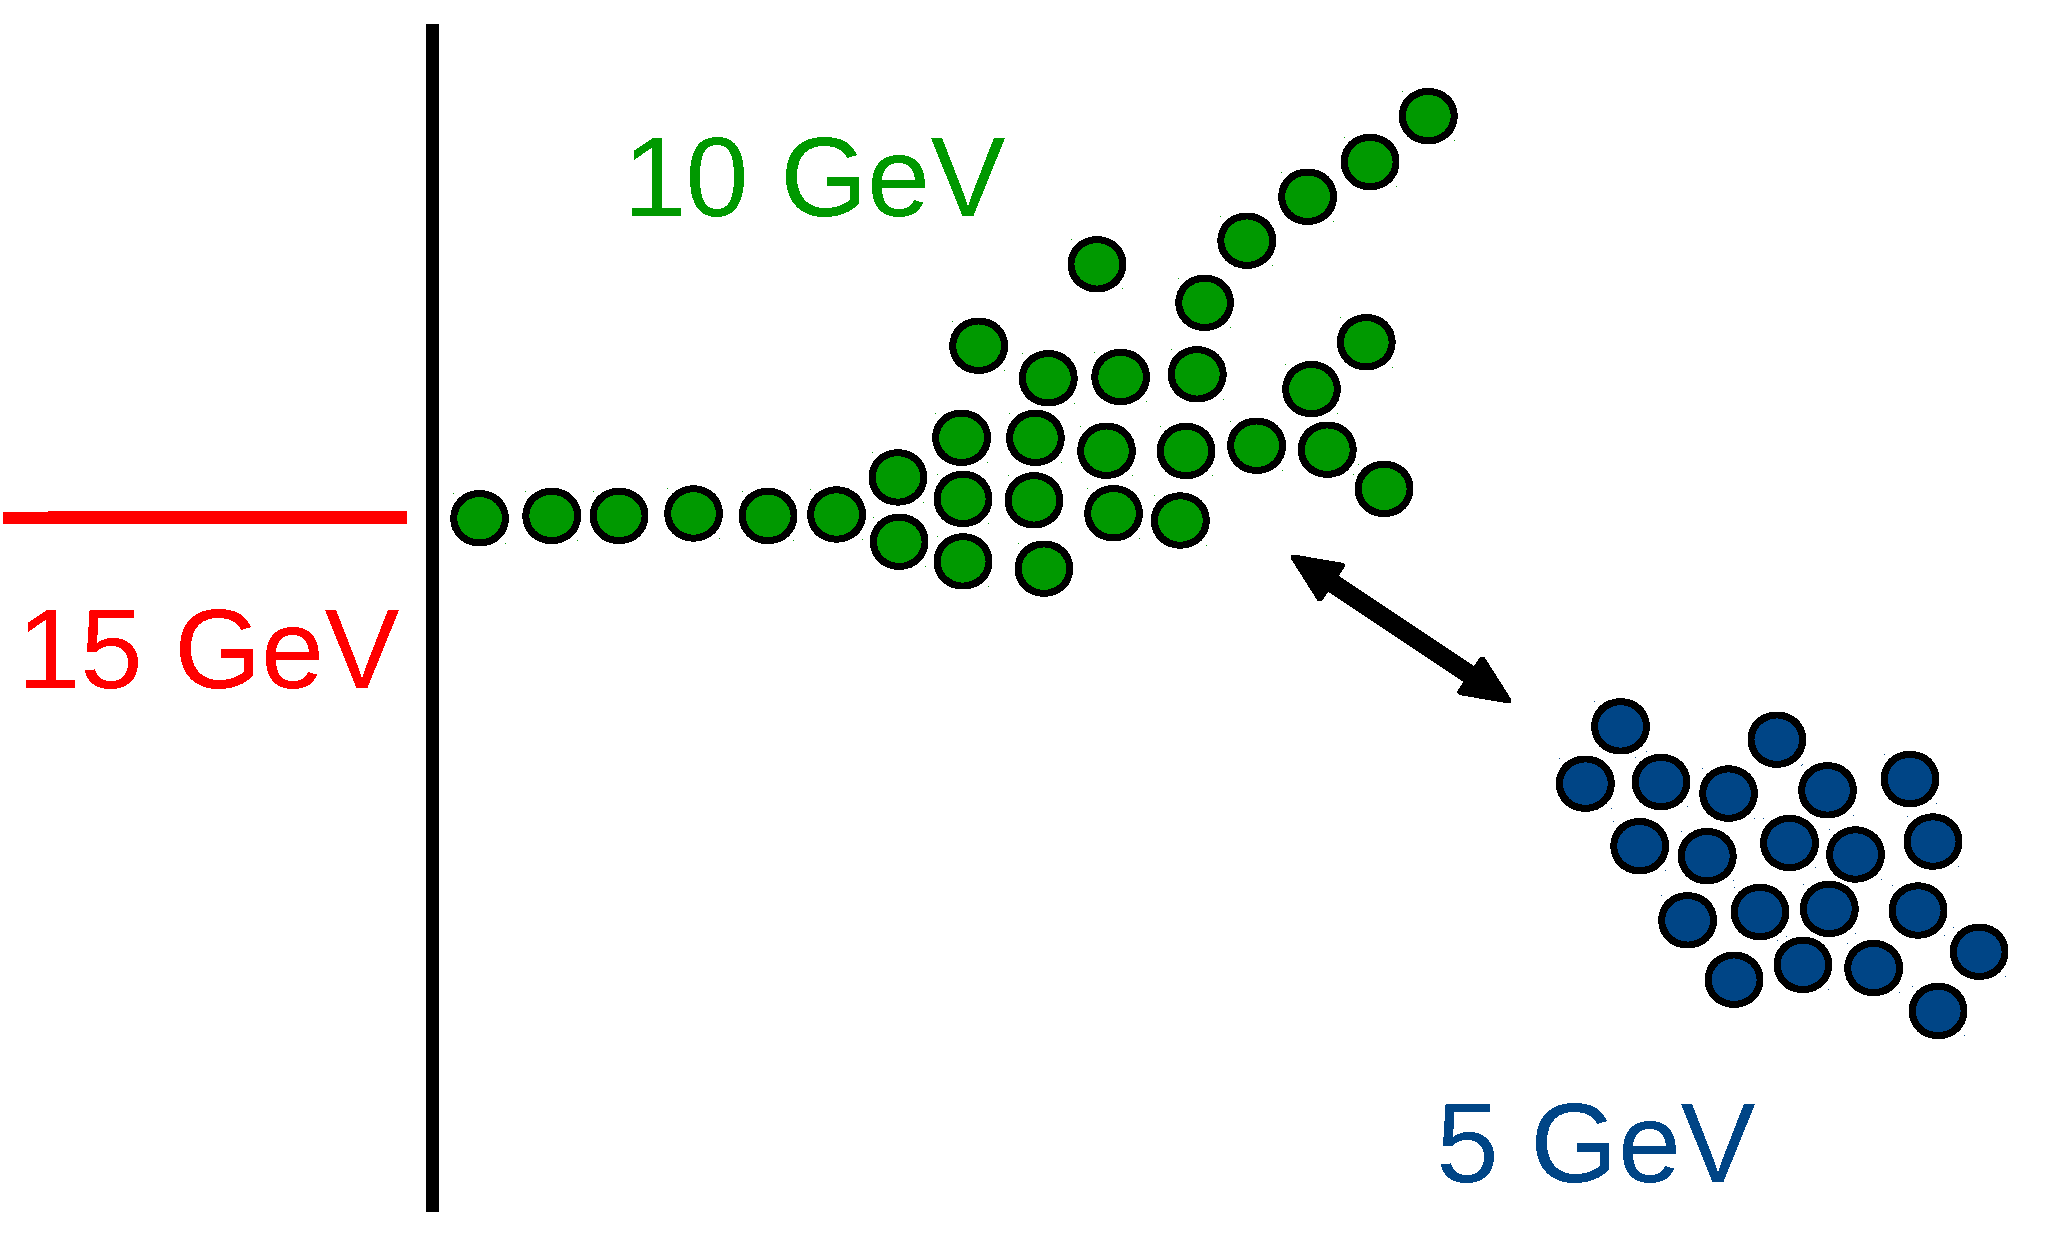
\includegraphics[width=0.8\linewidth]{TopologicalAssociationsIntro.pdf}
        \onslide<6> \centering 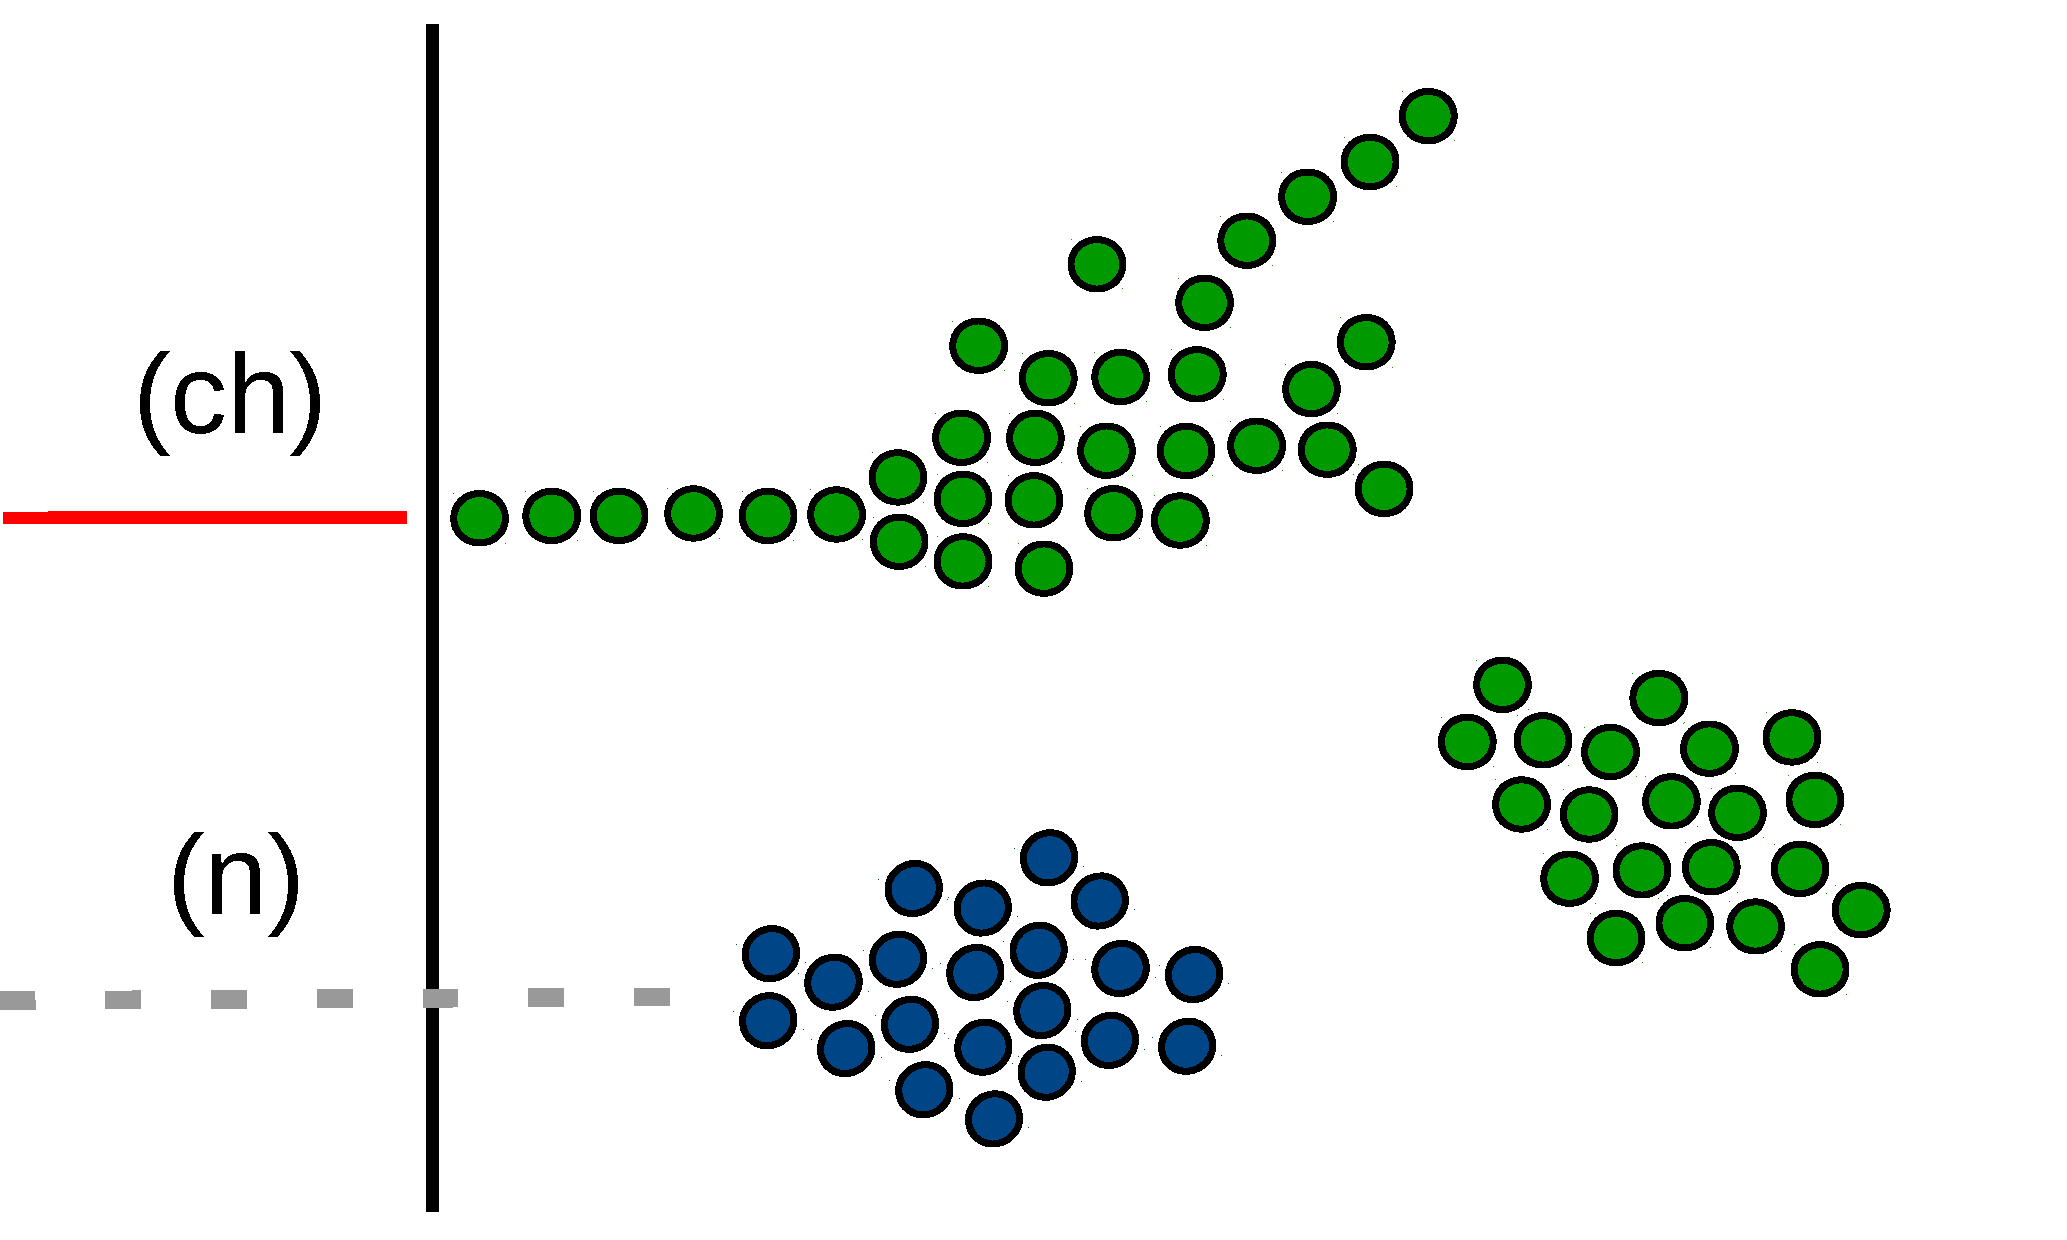
\includegraphics[width=0.8\linewidth]{PfoCreationIntro.pdf}
      \end{overprint}
    \end{minipage}
  \end{frame}


  \begin{frame}
  \frametitle{\secname}
  \framesubtitle{\subsecname - Connexions des vertex}
    \begin{overlayarea}{\textwidth}{0.6\textheight}
      \begin{center}
        \includegraphics[width=0.7\linewidth]<1>{ConnectorSeeding_1.pdf}
        \includegraphics[width=0.7\linewidth]<2>{ConnectorSeeding_2.pdf}
        \includegraphics[width=0.7\linewidth]<3>{ConnectorSeeding_3.pdf}
        \includegraphics[width=0.7\linewidth]<4>{ConnectorSeeding_4.pdf}
        \includegraphics[width=0.7\linewidth]<5>{ConnectorSeeding_5.pdf}
        \includegraphics[width=0.7\linewidth]<6>{ConnectorSeeding_6.pdf}
        \includegraphics[width=0.7\linewidth]<7>{ConnectorSeeding_7.pdf}
        \includegraphics[width=0.7\linewidth]<8>{ConnectorSeedingFinal.pdf}
      \end{center}
    \end{overlayarea}
  \end{frame}


  \begin{frame}
  \frametitle{\secname}
  \framesubtitle{\subsecname - Nettoyage des connexions}
    \begin{overlayarea}{\textwidth}{0.6\textheight}
      \begin{center}
        \includegraphics[width=0.7\linewidth]<1>{ConnectorCleaning_1.pdf}
      \end{center}
    \end{overlayarea}
  \end{frame}


  \begin{frame}
  \frametitle{\secname}
  \framesubtitle{\subsecname - Nettoyage des connexions}
    \begin{minipage}{0.3\linewidth}
      \onslide<1-5>{
        Vecteur de référence :
        \begin{align*}
          \vec{C}_{ref} = - w_{bck} . \sum_\sigma \sum_b \vec{c}_{b,\sigma} \\- w_{fwd} . \sum_\delta \sum_f \vec{c}_{f,\delta}
        \end{align*}
      }
      ~ \\
      \onslide<3-5>{
        Paramètre d'ordre :
        \begin{align*}
          \kappa = \Big(\frac{\theta}{\pi}\Big)^{p_\theta} . \Big( \frac{\Delta}{\Delta_{max}}\Big)^{p_\Delta}
        \end{align*}
      }
    \end{minipage}
    \begin{minipage}{0.68\linewidth}
      \begin{overlayarea}{\textwidth}{0.8\textheight}
        \begin{center}
          \vspace{10pt}
          \includegraphics[width=0.9\linewidth]<1>{ConnectorCleaning_2.pdf}
          \includegraphics[width=0.9\linewidth]<2>{ConnectorCleaning_3.pdf}
          \includegraphics[width=0.9\linewidth]<3>{ConnectorCleaning_3.pdf}
          \includegraphics[width=0.9\linewidth]<4>{ConnectorCleaning_4.pdf}
          \includegraphics[width=0.9\linewidth]<5>{ConnectorCleaning_5.pdf}
        \end{center}
      \end{overlayarea}
    \end{minipage}
  \end{frame}


  \begin{frame}
  \frametitle{\secname}
  \framesubtitle{\subsecname - Nettoyage des connexions}
    \begin{overlayarea}{\textwidth}{0.6\textheight}
      \begin{center}
        \includegraphics[width=0.7\linewidth]<1>{ConnectorCleaningFinal.pdf}
      \end{center}
    \end{overlayarea}
  \end{frame}


  \begin{frame}
  \frametitle{\secname}
  \framesubtitle{\subsecname - Hadrons isolés}
    \begin{center}
      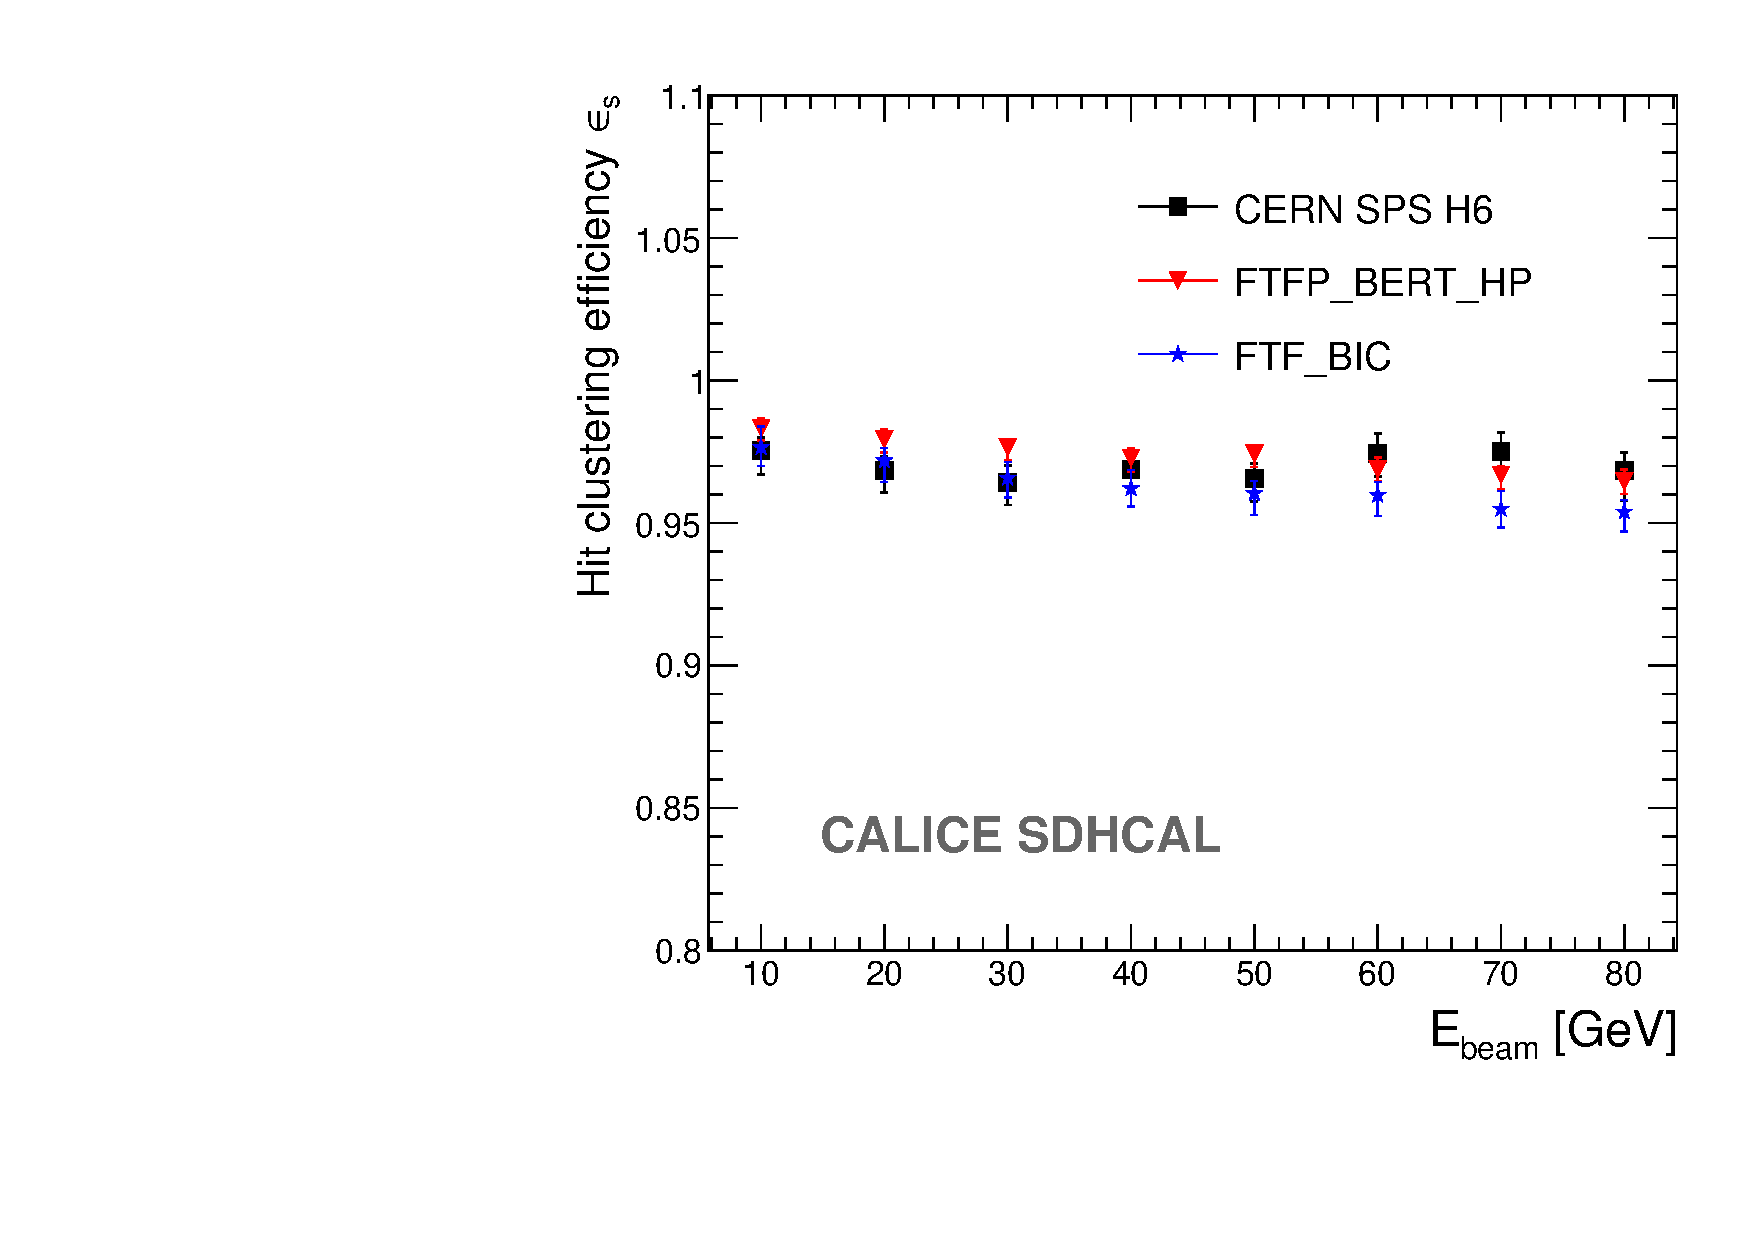
\includegraphics[width=0.49\linewidth]{Single_MC_DATA_COMP_Efficiency.pdf}
      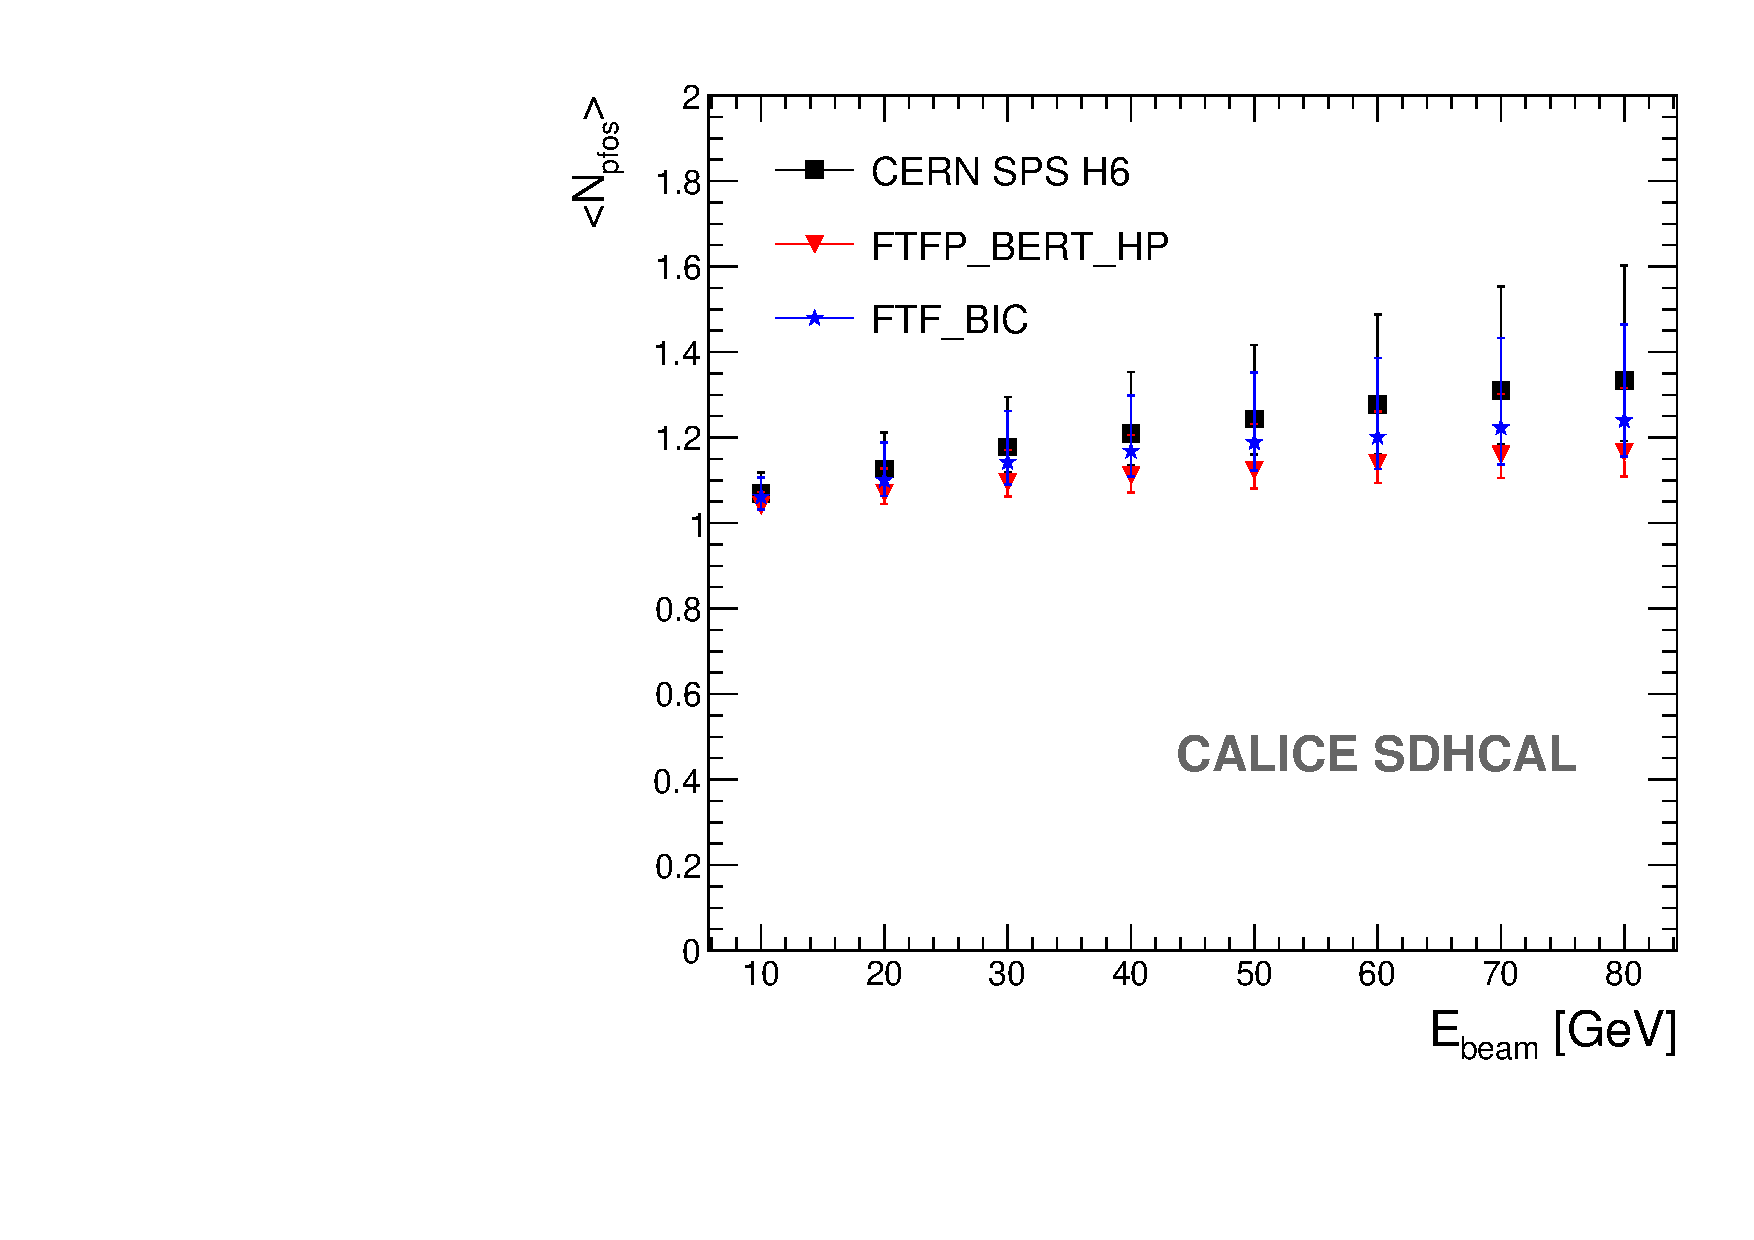
\includegraphics[width=0.49\linewidth]{Single_MC_DATA_COMP_NPfos.pdf}
    \end{center}
  \end{frame}

  \begin{frame}
  \frametitle{\secname}
  \framesubtitle{\subsecname - Hadrons isolés}
    \begin{center}
      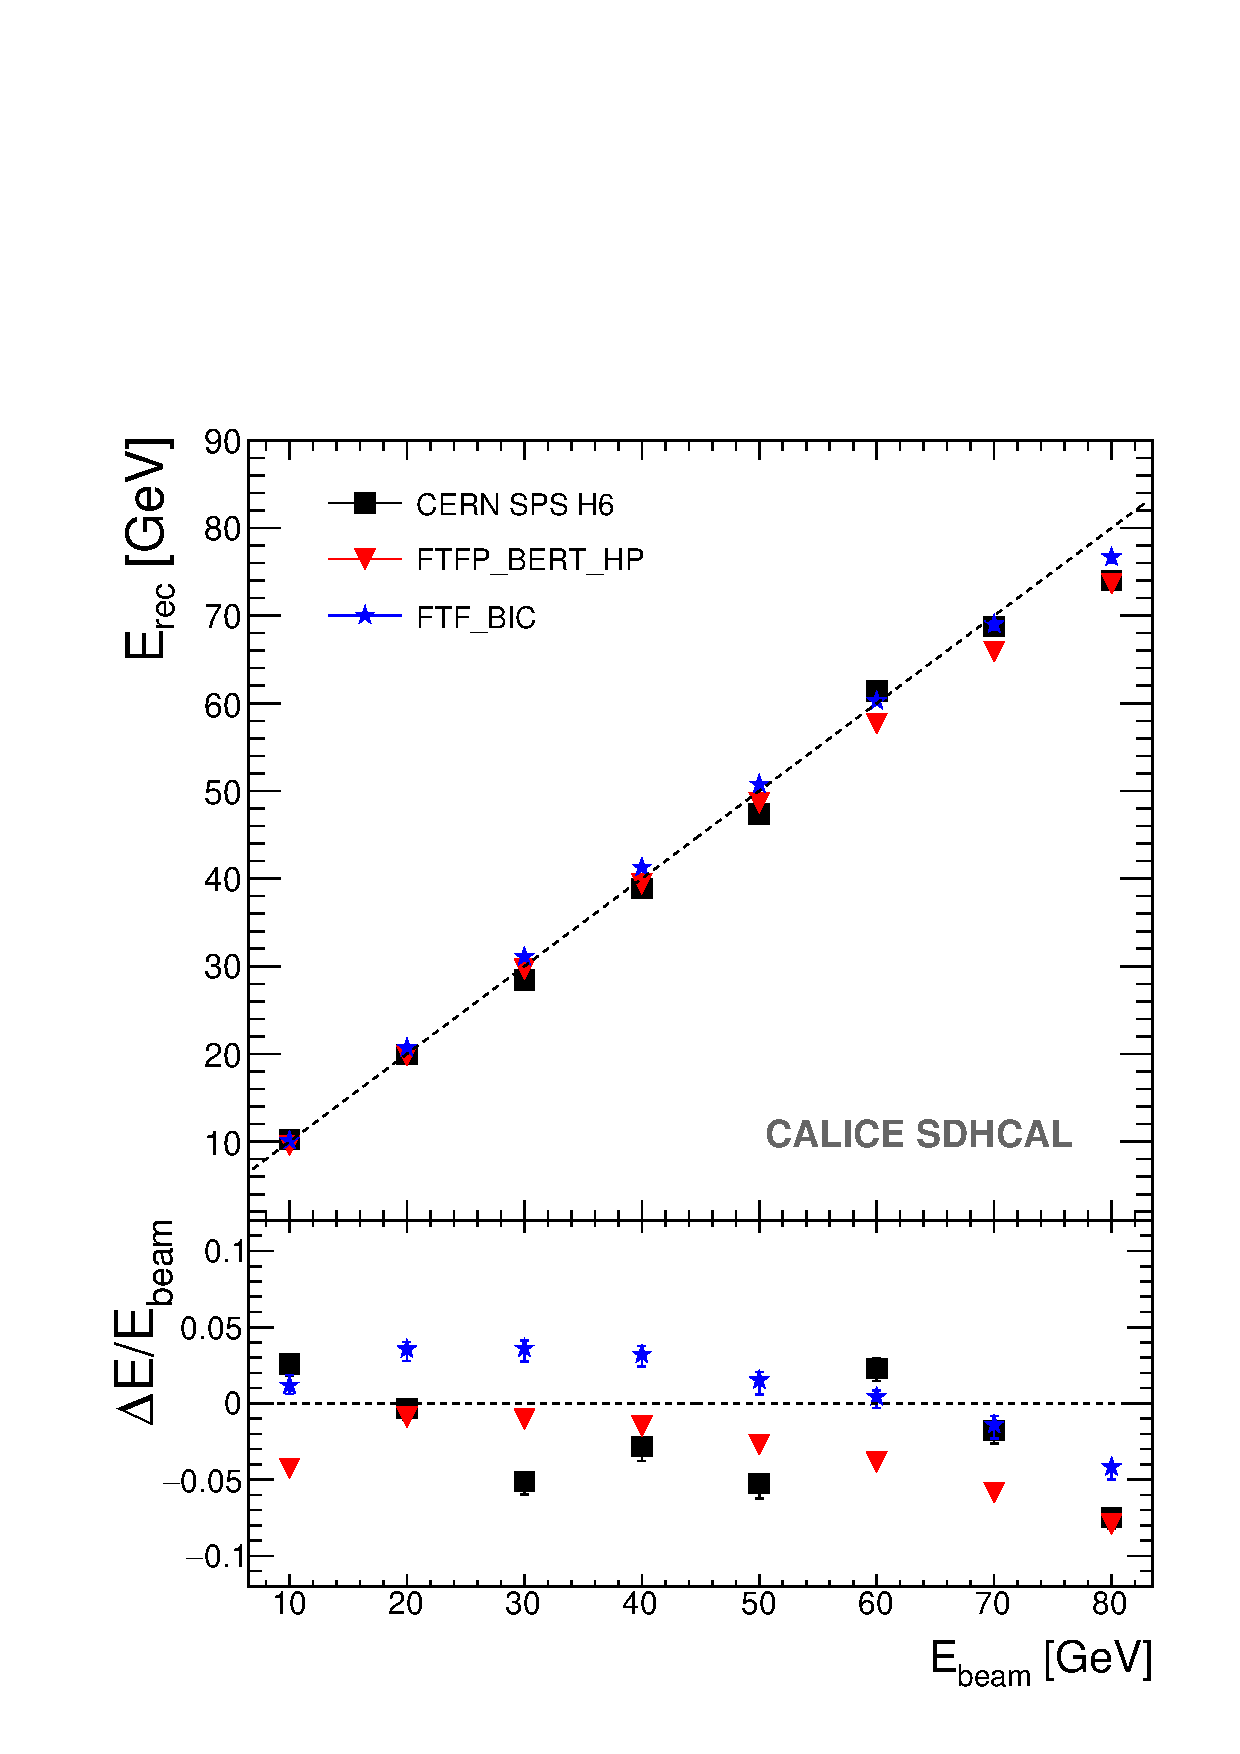
\includegraphics[width=0.49\linewidth]{Single_MC_DATA_COMP_ERec.pdf}
      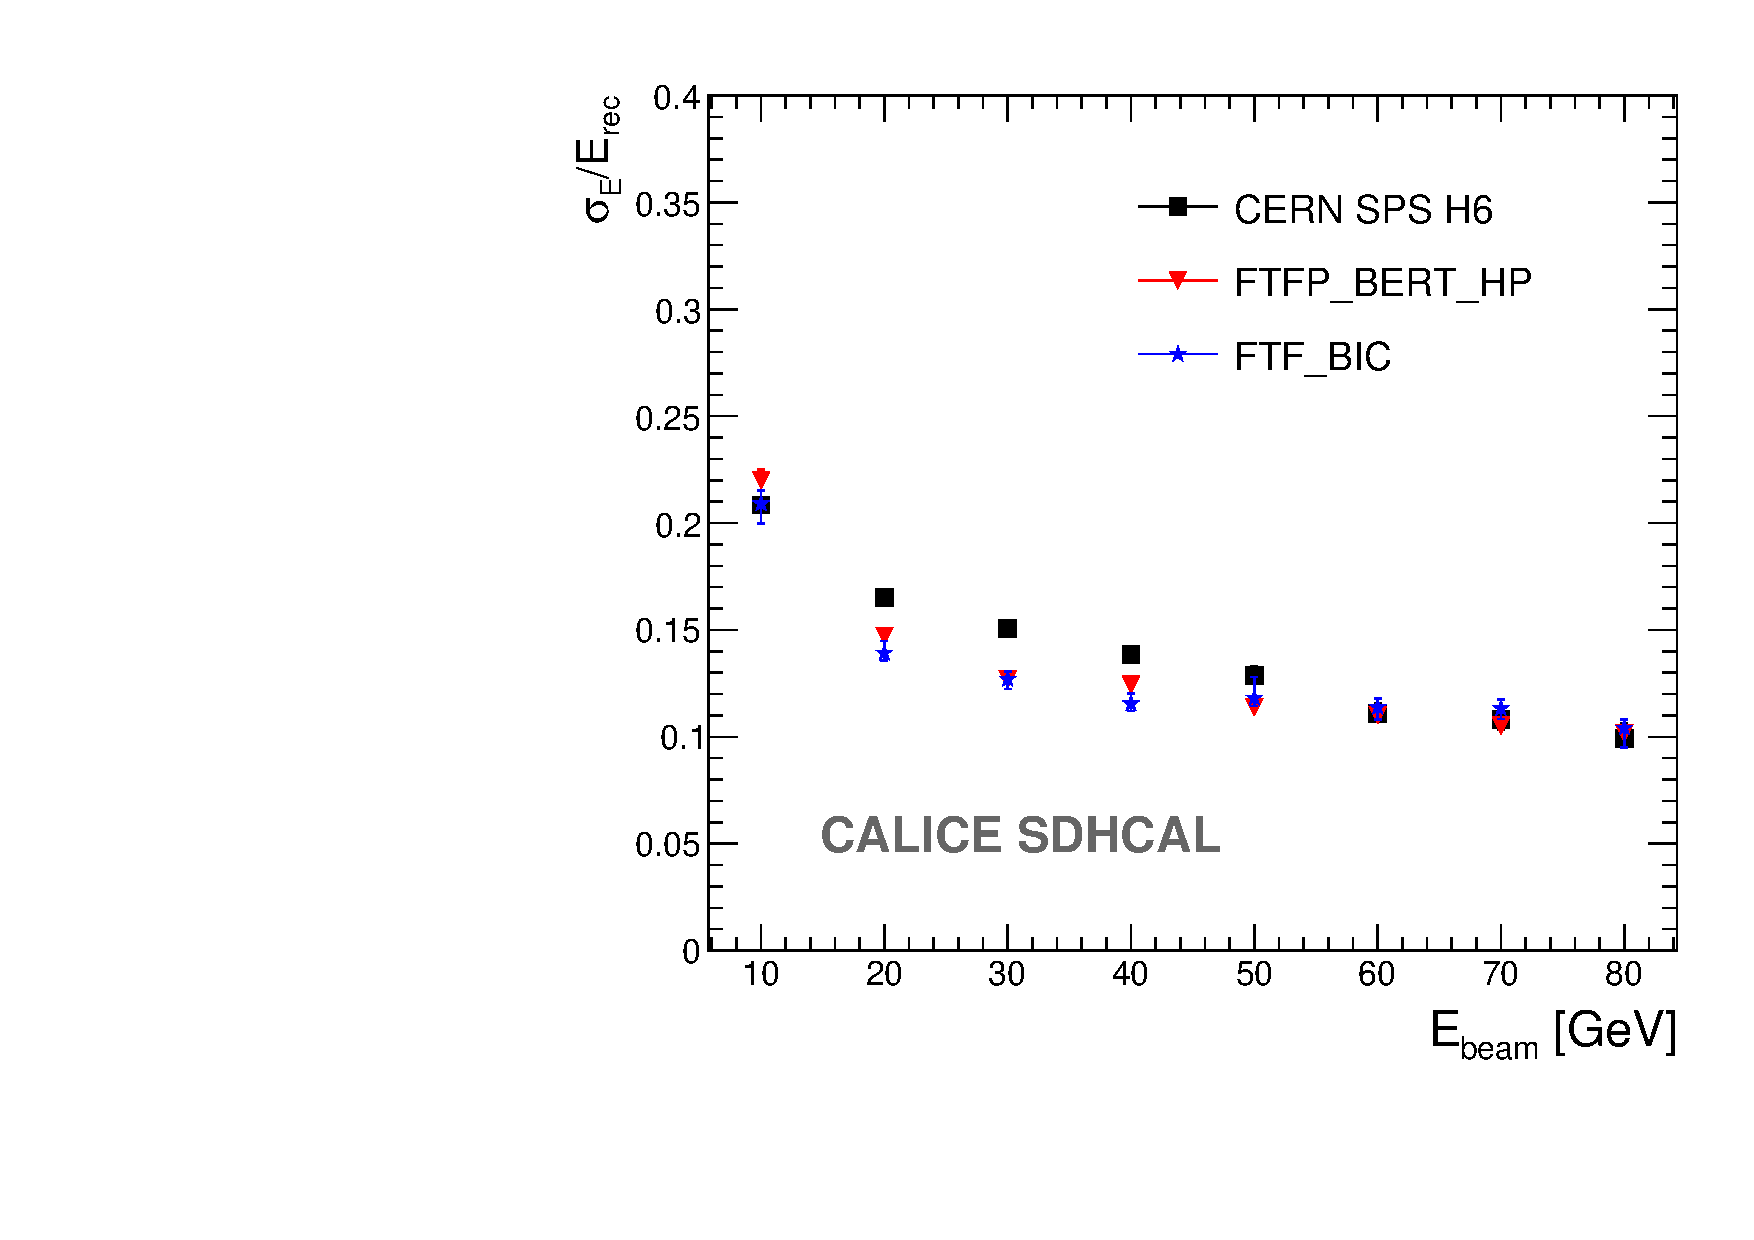
\includegraphics[width=0.49\linewidth]{Single_MC_DATA_COMP_EResol.pdf}
    \end{center}
  \end{frame}


  \begin{frame}
  \frametitle{\secname}
  \framesubtitle{\subsecname - Séparation de deux hadrons}
    \begin{block}{Superposition de deux événements hadronique}
      \begin{itemize}
        \item Détermination des points d'entrées et barycentres.
        \item Suppression des hits du segment de trace primaire du hadron de 10 GeV
        \item Centrage au centre du calorimètre (x et y) puis décalage de $\pm$ d/2 dans la direction x
        \item Hit superposé : le seuil le plus haut est assigné à ce hit
        \item Les hits sont étiqueté 1, 2 ou 3 (superposé).
      \end{itemize}
    \end{block}
    \begin{center}
      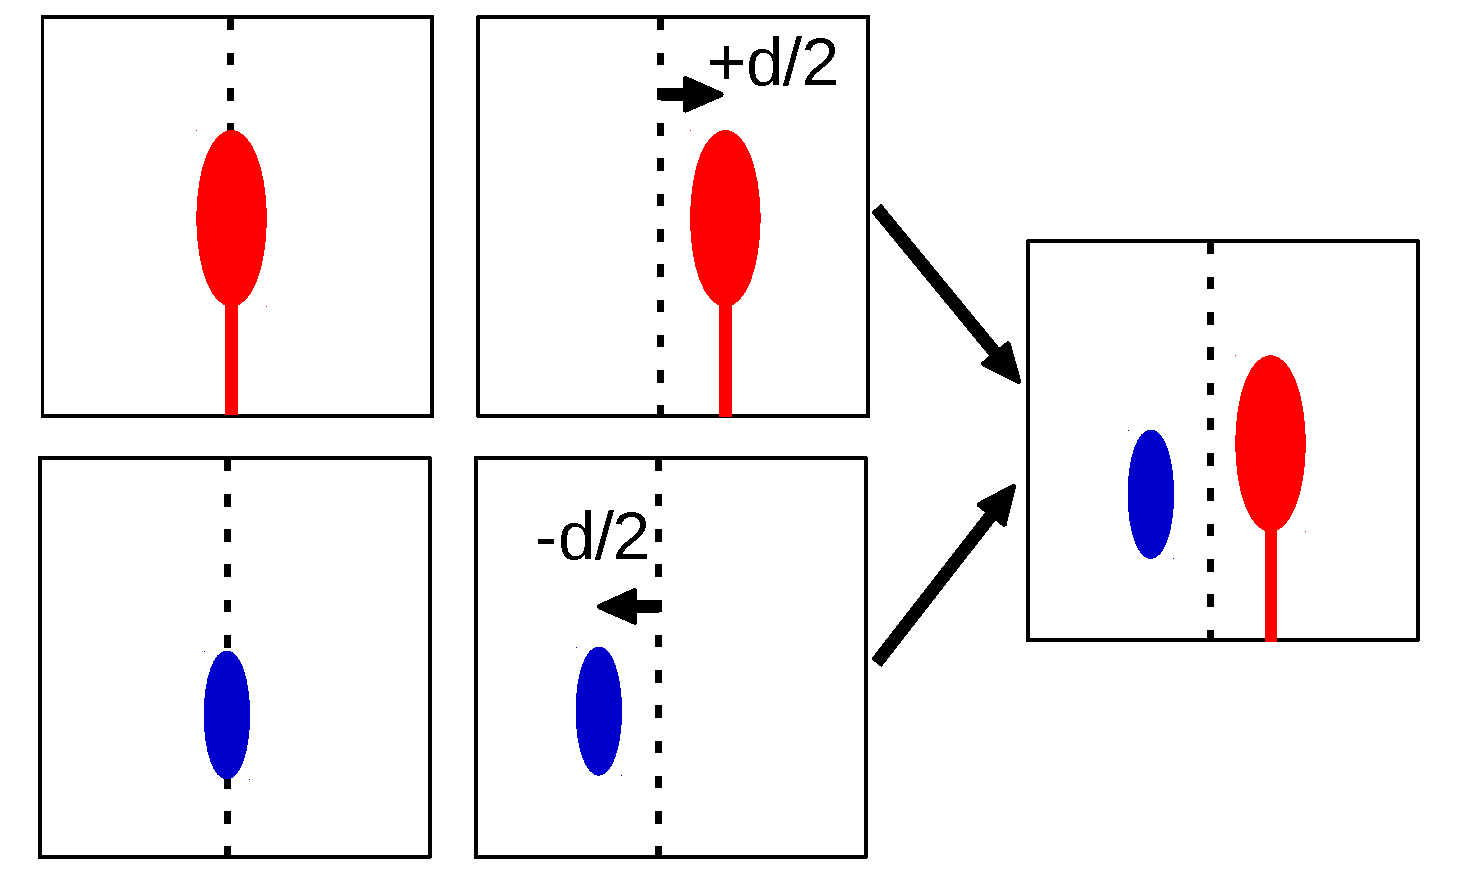
\includegraphics[width=0.65\linewidth]{OverlayEvent.pdf}
    \end{center}
  \end{frame}


  \begin{frame}
  \frametitle{\secname}
  \framesubtitle{\subsecname - Séparation de deux hadrons}
    \begin{center}
      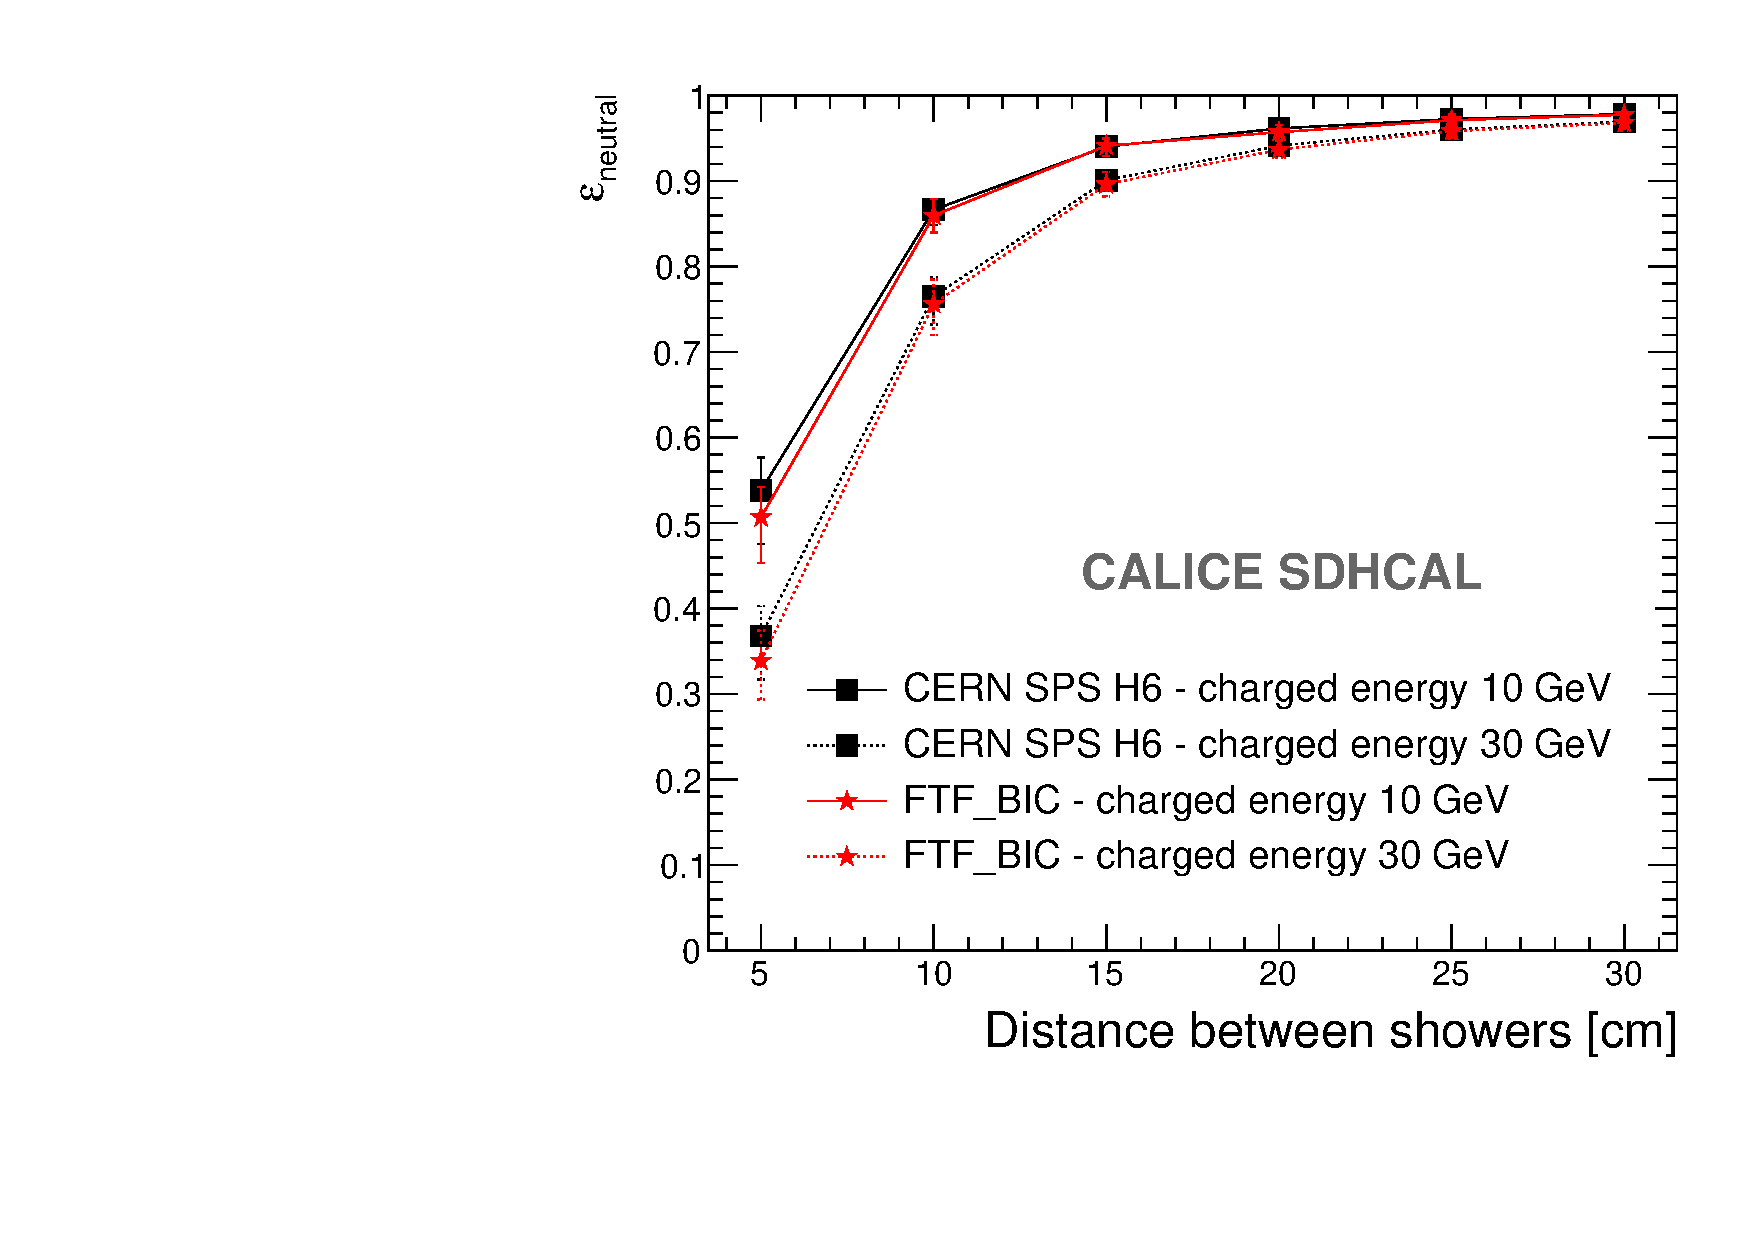
\includegraphics[width=0.49\linewidth]{OverlayEvent_Efficiency.pdf}
      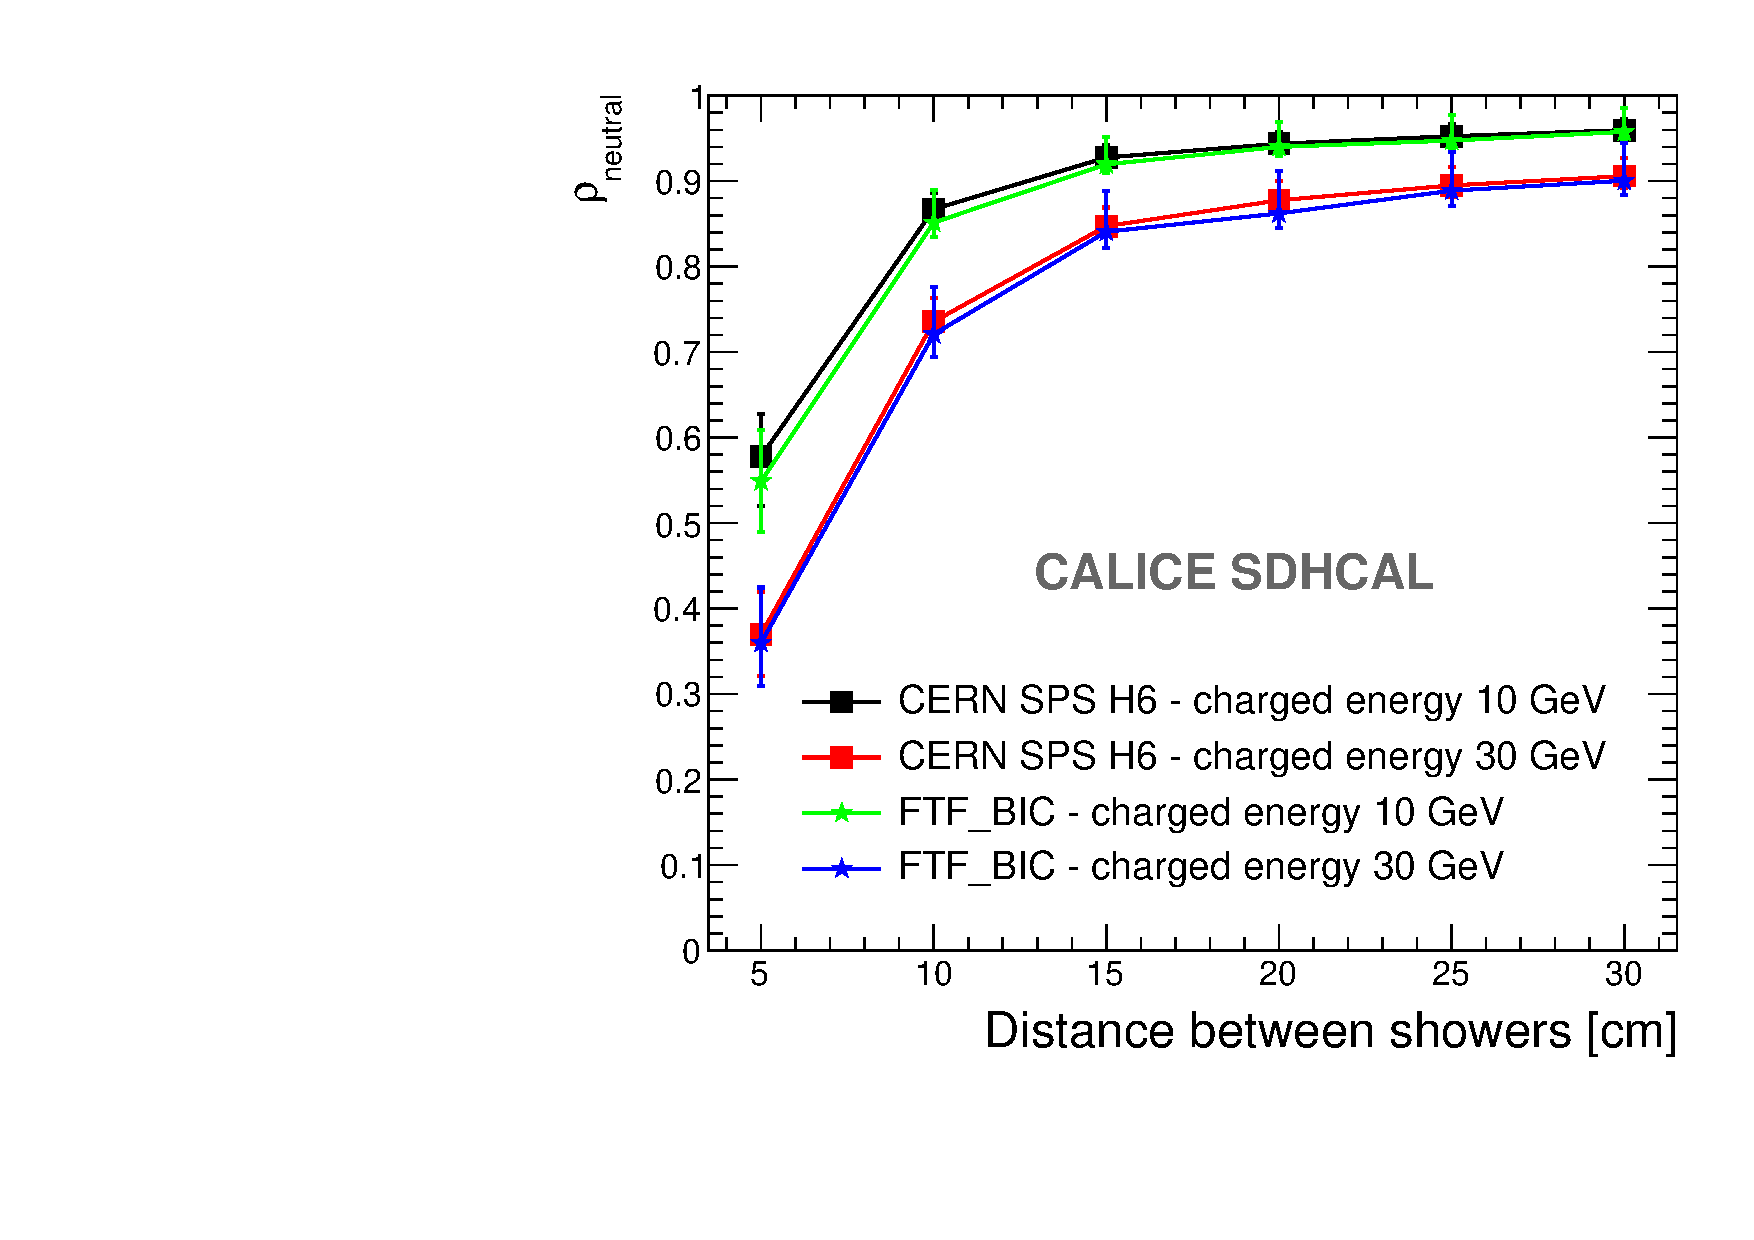
\includegraphics[width=0.49\linewidth]{OverlayEvent_Purity.pdf}
    \end{center}
  \end{frame}

  \begin{frame}
  \frametitle{\secname}
  \framesubtitle{\subsecname - Séparation de deux hadrons}
    \begin{center}
      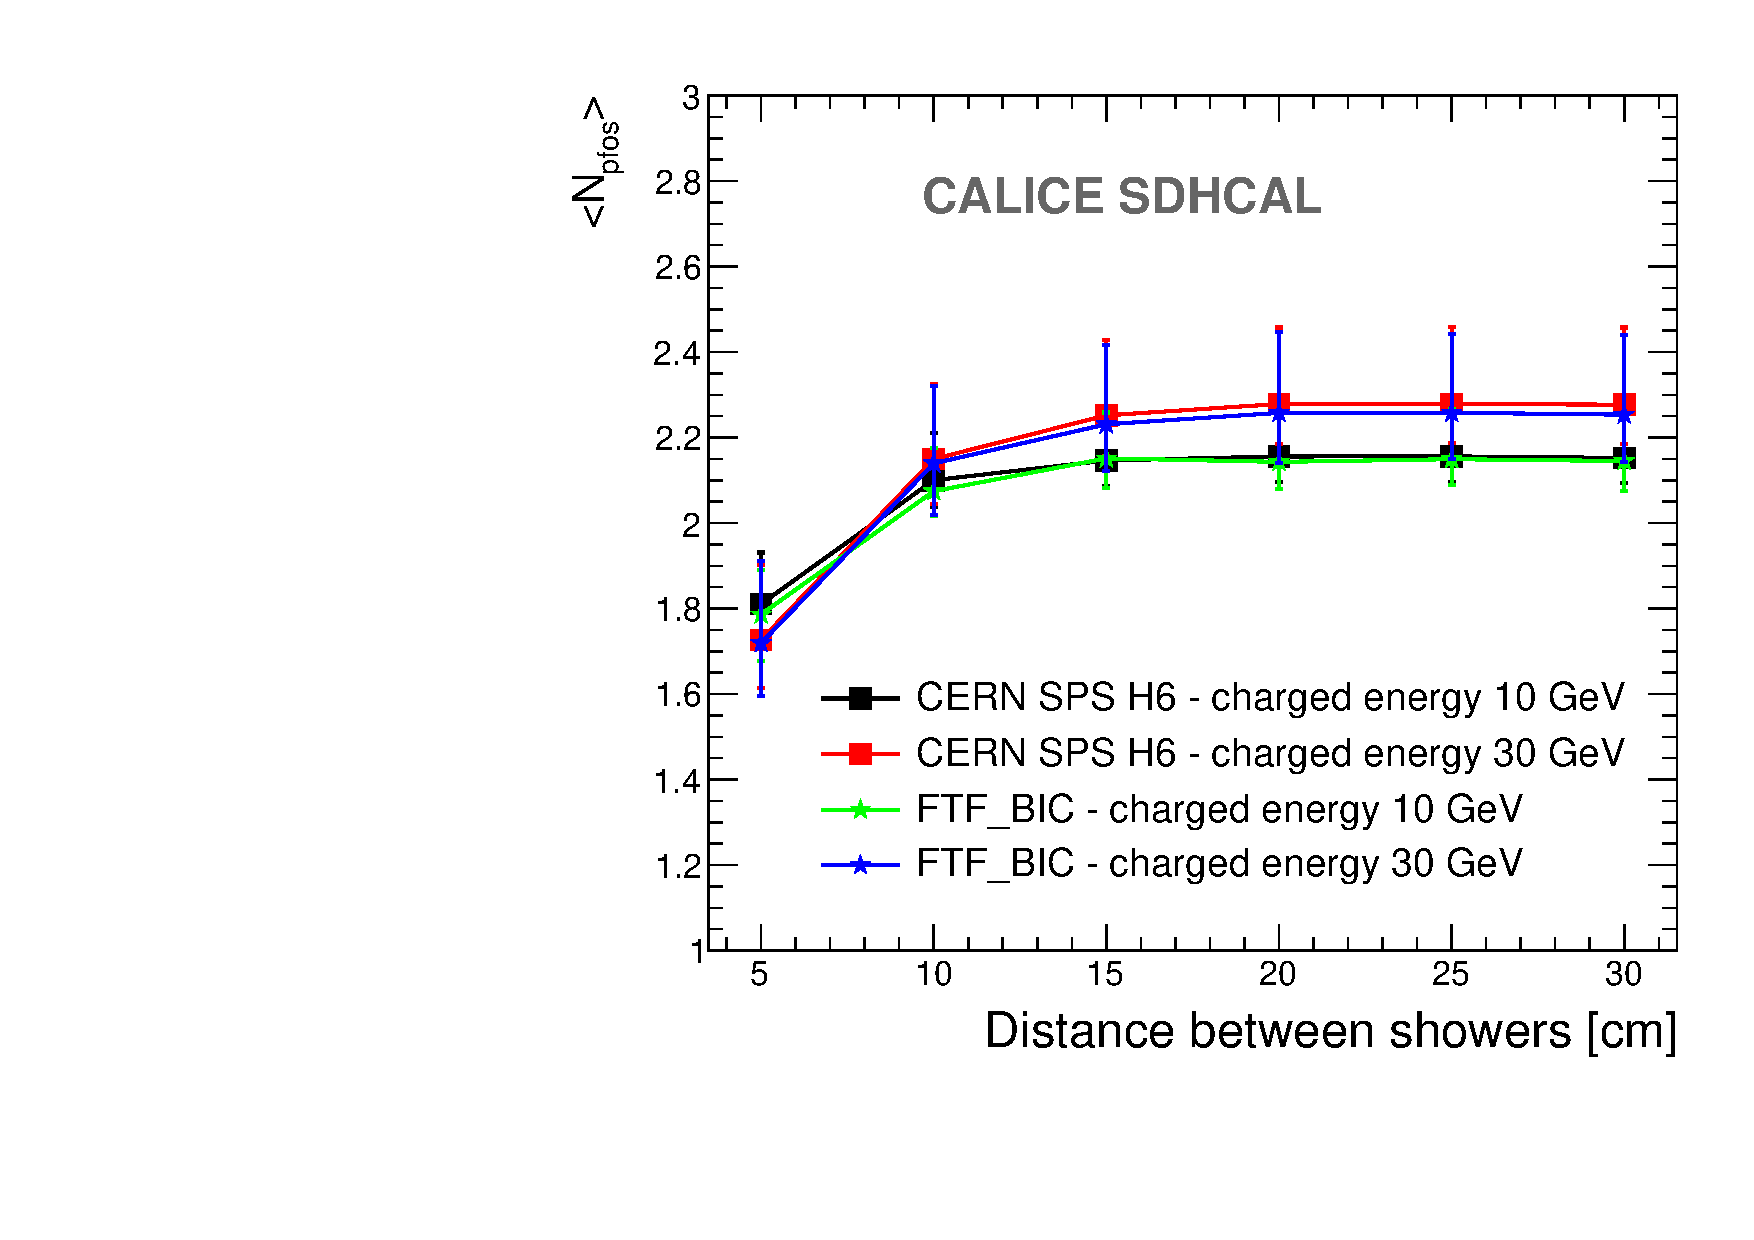
\includegraphics[width=0.49\linewidth]{OverlayEvent_NPfos.pdf}
      \includegraphics[width=0.49\linewidth]{OverlayEvent_EnergyDifference.pdf}
    \end{center}
  \end{frame}

  \begin{frame}
  \frametitle{\secname}
  \framesubtitle{\subsecname - Séparation de deux hadrons}
    \begin{center}
      \includegraphics[width=0.49\linewidth]{OverlayEvent_ProbaNeutral.pdf}
      \includegraphics[width=0.49\linewidth]{OverlayEvent_EnergyDifferenceEfficient.pdf}
    \end{center}
  \end{frame}



  %% ArborPFA - ILD
  \subsection{ArborPFA pour le détecteur ILD}

  \begin{frame}
  \frametitle{\secname}
  \framesubtitle{\subsecname}
    \begin{minipage}{0.53\linewidth}
      \begin{block}{ArborPFA pour le détecteur ILD}
        \begin{itemize}
          \item Prise en compte des autres sous détecteurs
          \begin{itemize}
            \item Connexion/nettoyage dans le ECAL
            \item Connexion ECAL-HCAL
            \item Traces courbées dans la TPC
          \end{itemize}
          \item Étude de linéarité et de résolution en énergie pour les hadrons neutres $K_{0}^{L}$
          \begin{itemize}
            \item Calibration initiale de référence \\
            $\rightarrow$ $\phi=0$ et $\theta=1.5$ $rad$
            \item Correction en énergie près des interstices dans le tonneau central (5 modules)
            \item Correction en énergie en fonction de l'angle $\theta$
          \end{itemize}
          \item Performances physiques sur un système di-jets ($Z^0~\rightarrow q\bar{q}$)
          \begin{itemize}
            \item Linéarité, résolution en énergie
            \item Contribution de différents termes de confusions
          \end{itemize}
        \end{itemize}
      \end{block}
    \end{minipage} ~~~~\hfill
    \begin{minipage}{0.43\linewidth}
      \begin{center}
        \includegraphics[width=\linewidth]{BarrelEndcapRegions.pdf}
      \end{center}
    \end{minipage}
  \end{frame}



  \begin{frame}
  \frametitle{\secname}
  \framesubtitle{\subsecname - Calibration et corrections en énergie}
    \begin{minipage}{0.6\linewidth}
      \begin{block}{Calibration initiale ($\phi=0$, $\theta=1.5$ $rad$)}
        \begin{itemize}
          \item Kaons neutres $K_{0}^{L}$, $E$ $=$ $[10, 80]~GeV$
          \item Estimateur d'énergie :
          \begin{align*}
            E_{rec} = \sum_{i} \big(c_{h}^{e}.e_i\big) + \big(\alpha.N_1 + \beta.N_2 + \gamma.N_3\big)
          \end{align*}
          avec :
          \begin{itemize}
            \item $c_{h}^{e}$ = 1.075 $GeV$
            \item $\alpha$ = 0.0433(771) $\pm 10^{-4}$ $GeV$
            \item $\beta$  = 0.0884(24)  $\pm 10^{-4}$ $GeV$
            \item $\gamma$ = 0.4573(53)  $\pm 10^{-4}$ $GeV$
          \end{itemize}
        \end{itemize}
      \end{block}
      \begin{center}
        \includegraphics[width=0.6\linewidth]{ERecLin.pdf}
      \end{center}
    \end{minipage} \hfill
    \begin{minipage}{0.39\linewidth}
      \begin{center}
        \includegraphics[width=0.8\linewidth]{kaon0L_primary_calibration_erec_2.pdf} \\
        \includegraphics[width=0.8\linewidth]{kaon0L_primary_calibration_eresol_2.pdf}
      \end{center}
    \end{minipage}
  \end{frame}


  \begin{frame}
  \frametitle{\secname}
  \framesubtitle{\subsecname - Calibration et corrections en énergie}
    \begin{minipage}{0.49\linewidth}
      \begin{block}{Correction près des interstices}
        \begin{itemize}
          \item Tonneau central séparé en 5 modules
          \item Budget matière plus important près des interstices \\
          $\rightarrow$ Énergie manquante !
          \item Correction en énergie :\\
          Comptage de l'énergie déposé près des interstices $E_{gap}$
          \begin{align*}
            E_{rec,gap} = E_{rec} + \alpha_{gap}.E_{gap}
          \end{align*}
          avec $\alpha_{gap}$ = 1.5254
        \end{itemize}
      \end{block}
      \begin{center}
        \includegraphics[width=\linewidth]{ModuleGap.pdf}
      \end{center}
    \end{minipage} \hfill
    \begin{minipage}{0.5\linewidth}
      \begin{center}
        \begin{overprint}
          \onslide<1> \centering \includegraphics[width=0.8\linewidth]{ERecLin.pdf} \\ \includegraphics[width=0.8\linewidth]{ERes_thesis.pdf}
          \onslide<2> \centering \includegraphics[width=0.8\linewidth]{ERecLinGap_nofit_thesis.pdf} \\ \includegraphics[width=0.8\linewidth]{EResLinGap_thesis.pdf}
        \end{overprint}
      \end{center}
    \end{minipage}
  \end{frame}


  \begin{frame}
  \frametitle{\secname}
  \framesubtitle{\subsecname - Calibration et corrections en énergie}
    \begin{minipage}{0.49\linewidth}
      \begin{block}{Correction en fonction de $cos\theta$}
        \begin{itemize}
          \item<1-> Chute linéaire de l'énergie dans le tonneau et les bouchons
          \item<2-> Énergies : ajustement linéaire  dans les régions 1 et 3
          \item<3-> Paramètres : ajustement d'un polynôme d'ordre 1 ou 2
          \item<4-> Région intermédiaire 2 : correction en fonction des fractions tonneau/bouchon
          % \item<>
        \end{itemize}
      \end{block}
      \begin{center}
        \begin{overprint}
          \onslide<2> \centering \includegraphics[width=0.8\linewidth]{ThetaCalibFit_nofit_thesis.pdf}
          \onslide<3> \centering \includegraphics[width=0.8\linewidth]{ThetaCalibFit_pol2_thesis.pdf}
          \onslide<4-> \centering \includegraphics[width=0.8\linewidth]{EndcapFraction_thesis.pdf}
        \end{overprint}
      \end{center}
    \end{minipage} \hfill
    \begin{minipage}{0.5\linewidth}
      \begin{center}
        \begin{overprint}
          \onslide<1> \centering \includegraphics[width=0.8\linewidth]{ERecLinGap_nofit_thesis.pdf} \\ \includegraphics[width=0.8\linewidth]{EResLinGap_thesis.pdf}
          \onslide<2-4> \centering \includegraphics[width=0.8\linewidth]{ERecLinGap_fits_thesis.pdf} \\ \includegraphics[width=0.8\linewidth]{EResLinGap_thesis.pdf}
          \onslide<5-> \centering \includegraphics[width=0.8\linewidth]{ERecCorrThetaGapO2_thesis.pdf} \\ \includegraphics[width=0.8\linewidth]{EResCorrThetaGapO2_thesis.pdf}
        \end{overprint}
      \end{center}
    \end{minipage}
  \end{frame}


  \begin{frame}
  \frametitle{\secname}
  \framesubtitle{\subsecname - Les algorithmes de reconstruction}
    \begin{block}{Implémentation pour le détecteur ILD}
      \begin{itemize}
        \item<1-> Préparation de l'évenement (2 algos)
        \item<2-> Reconstruction des photons (8 algos)
        \item<3-> Clustering principal (11 algos)
        \begin{itemize}
          \item<4-> Connexion des vertex et nettoyage des connexions (3 algos)
          \item<5-> Associations topologiques (1+7 algos)
        \end{itemize}
        \item<6-> Reclustering (41 algos)
        \begin{itemize}
          \item<6-> Reclustering en cas d'excès en énergie (12 clust + 7 top + 1 trk-cl)
          \item<6-> Reclustering en cas d'énergie manquante (12 clust + 7 top + 1 trk-cl)
          \item<6-> Reclustering en cas d'associations trace-cluster multiples (1 algo)
        \end{itemize}
        \item<7-> Création et identification des particules reconstruites (6 algos)
      \end{itemize}
    \end{block}
    ~ \\
    \begin{overprint}
      \onslide<2-3> \centering \includegraphics[width=0.8\linewidth]{NearbyTrackPhotonRemovalILD.pdf}
      \onslide<4> \centering \includegraphics[width=0.8\linewidth]{TrackDrivenSeeding.pdf}
      \onslide<5> \centering \includegraphics[width=0.8\linewidth]{ILDTopologicalAssociations.pdf}
      \onslide<6-> \centering \includegraphics[width=0.8\linewidth]{ReclusteringAlgorithmsILD.pdf}
    \end{overprint}
  \end{frame}


  \begin{frame}
  \frametitle{\secname}
  \framesubtitle{\subsecname - Les performances physiques}
    \begin{minipage}{0.49\linewidth}
      \begin{center}
        \includegraphics[width=\linewidth]{ILDArborPFA_ErecConfusions_NoNeutralHadron.pdf}
      \end{center}
    \end{minipage}
    \begin{minipage}{0.49\linewidth}
      \begin{center}
        \includegraphics[width=\linewidth]{ILDArborPFA_EResol_NoNeutralHadron.pdf}
      \end{center}
    \end{minipage}
  \end{frame}

  \begin{frame}
  \frametitle{\secname}
  \framesubtitle{\subsecname - Les performances physiques}
    \begin{minipage}{0.49\linewidth}
      \begin{center}
        \includegraphics[width=\linewidth]{ILDArborPFA_Resolution_NoNeutralHadron.pdf}
      \end{center}
    \end{minipage}
    \begin{minipage}{0.49\linewidth}
      \begin{center}
        \includegraphics[width=\linewidth]{ILDArborPFA_PerfectResolution_NoNeutralHadron.pdf}
      \end{center}
    \end{minipage}
  \end{frame}




















  %%%%%%%%%%%%%
  %% DQM4HEP %%
  %%%%%%%%%%%%%
  \section{Logiciel de surveillance de données}

  \begin{frame}
  \frametitle{\secname}
    \tableofcontents[currentsection]
  \end{frame}

  \subsection{Introduction}

  %% Introduction
  \begin{frame}
  \frametitle{\secname}
  \framesubtitle{\subsecname}
  \small
    \begin{block}{Les systèmes de DQM}
      \begin{itemize}
        \item Évalue la \textbf{qualité} des données :
        \begin{itemize}
          \item en ligne
          \item hors ligne
        \end{itemize}
        \item \textbf{Alerte} l'utilisateur d'un \textbf{état anormal du système} de détection (fuite de gaz, cellule morte, ...)
        \item Présents dans les expériences de physique de hautes énergies. Par exemple :
        \begin{itemize}
          \item CMS   - CMSSW DQM
          \item ALICE - AMORE
        \end{itemize}
        \item Principe général : collecter $\rightarrow$ distribuer $\rightarrow$ analyser $\rightarrow$ visualiser
      \end{itemize}
    \end{block}
    \pause
    \begin{minipage}{0.47\linewidth}
      \begin{block}{Fonctionnalités communes}
        \begin{itemize}
          \item Couplage au système d'acquisition
          \item Analyse de données en ligne / hors ligne
          \item Tests de la qualité des données
          \item Interface de visualisation des données (histogrammes, scalaires, etc ...)
          \item Environnements distribués \\(multi-processus + réseau)
        \end{itemize}
      \end{block}
    \end{minipage} \hfill
    \begin{minipage}{0.47\linewidth}
      \pause
      \begin{block}{Fonctionnalités différentes}
        \begin{itemize}
          \item \textbf{Contenu des données entrantes}
          \item \textbf{Format des données entrantes}
          \item Contenu des analyses
          \item Couplage au système d'acquisition
          \item Synthèse différente des données sur l'interface utilisateur
        \end{itemize}
      \end{block}
    \end{minipage}
    \pause
    \begin{center} \textbf{Logiciel commun ???} \end{center}
  \end{frame}


  \subsection{Logiciel DQM4HEP}

  %% DQM4HEP introduction
  \begin{frame}
  \frametitle{\secname}
  \framesubtitle{\subsecname}
    \begin{block}{Points clés}
      \begin{itemize}
        \item Nouveau logiciel : DQM4HEP (\textit{\textbf{D}ata \textbf{Q}uality \textbf{M}onitoring for \textbf{H}igh \textbf{E}nergy \textbf{P}hysics})
        \item Regroupement des fonctionnalités communes des différents logiciels
        \item \textbf{Abstraction des autres fonctionnalités}
      \end{itemize}
    \end{block}
    \pause
    \begin{block}{Les fonctionnalités}
      \begin{itemize}
        \item \textbf{Système de plug-in}
        \item \textbf{Abstraction des événements (modèle/format)}
        \item Station de gestion des runs
        \item Environnement d'analyse de données dédié au DQM
        \item Environnement distribué (serveur/client)
        \begin{itemize}
          \item Données brutes (DAQ)
          \item Éléments de surveillance (histogrammes, graphes, ...)
        \end{itemize}
        \item Interface graphique de visualisation (opérateurs)
      \end{itemize}
    \end{block}
  \end{frame}

  %% Architecture
  \begin{frame}
  \frametitle{\secname}
  \framesubtitle{\subsecname - architecture logicielle}
    \begin{center}
      \includegraphics[width=\linewidth]{GlobalArchitectureDiagram.pdf}
    \end{center}
    \pause
    \begin{tikzpicture}
      \draw[red,  thick, overlay] (2.15,2.1) rectangle (3.6,3);
      \draw[red,  thick, overlay] (4.3,3.7) rectangle (5.75,4.55);
      \draw[red,  thick, overlay] (9.05,0.75) rectangle (10.75,6.15);
    \end{tikzpicture}
  \end{frame}

  %% Analysis module
  \begin{frame}
  \frametitle{\secname}
  \framesubtitle{\subsecname - analyse des données provenant des détecteurs}
    \begin{minipage}{0.78\textwidth}
      \begin{block}{Module d'analyse de données}
        \begin{itemize}
          \item Conçu pour l'analyse de données (raw data, tracking, PFA, etc ...)
          \item Produit des élements de surveillance (histogrammes, graphes, ...)
          \item Évalue la qualité des données (Q-tests)
          \item Structuré en séquence de runs et de cycles
        \end{itemize}
      \end{block}
      \begin{center}
        \includegraphics[width=\linewidth]{AnalysisModuleApplicationDiagram.pdf}
      \end{center}
    \end{minipage} \hfill
    \begin{minipage}{0.18\textwidth}
      \begin{flushright}
        \begin{tikzpicture}[scale=0.8]
        \node[draw] (I) at (0,-1) {Init};
        \node[draw] (SR) at (0,-2) {Start of run};
        \node[draw] (SC) at (0,-3) {Start of cycle};
        \node[draw] (PE) at (0,-4) {Process event};
        \node[draw] (EC) at (0,-5) {End of cycle};
        \node[draw] (ER) at (0,-6) {End of run};
        \node[draw] (E) at (0,-7) {End};
        \tikzset{fleche/.style={->,>=latex,thick}}
        \draw[fleche] (0,0) node {$\bullet$} -- (I);
        \draw[fleche] (I) -- (SR);
        \draw[fleche] (SR) -- (SC);
        \draw[fleche] (SC) -- (PE);
        \draw[fleche] (PE) -- (EC);
        \draw[fleche] (EC) -- (ER);
        \draw[fleche] (ER) -- (E);
        \draw[fleche] (E) -- (0,-8) node {$\bullet$};
        \draw[fleche] (0,-4.5) -- (1.3,-4.5) -- (1.3,-3.5) -- (0,-3.5);
        \draw[fleche] (0,-5.5) -- (1.4,-5.5) -- (1.4,-2.5) -- (0,-2.5);
        \draw[fleche] (0,-6.5) -- (1.5,-6.5) -- (1.5,-1.5) -- (0,-1.5);
        \end{tikzpicture}
      \end{flushright}
    \end{minipage}
  \end{frame}

  %% Slow control module
  \begin{frame}
  \frametitle{\secname}
  \framesubtitle{\subsecname - analyse des données environnementales}
    \begin{minipage}{0.78\textwidth}
      \begin{block}{Module environnemental}
        \begin{itemize}
          \item Traitement de données environnementales (T, P, HV, gaz, ...)
          \item Pas de donnée transmise au module
          \item Produit des éléments de surveillance (histogrammes, graphes, ...)
          \item Évalue la qualité des données (Q-tests)
        \end{itemize}
      \end{block}
      \begin{center}
        \includegraphics[width=\linewidth]{StandaloneModuleApplicationDiagram.pdf}
      \end{center}
    \end{minipage} \hfill
    \begin{minipage}{0.18\textwidth}
      \begin{flushright}
        \begin{tikzpicture}[scale=0.8]
        \node[draw] (I) at (0,-1) {Init};
        \node[draw] (SC) at (0,-2) {Start of cycle};
        \node[draw] (PE) at (0,-3) {Process};
        \node[draw] (EC) at (0,-4) {End of cycle};
        \node[draw] (E) at (0,-5) {End};
        \tikzset{fleche/.style={->,>=latex,thick}}
        \draw[fleche] (0,0) node {$\bullet$} -- (I);
        \draw[fleche] (I) -- (SC);
        \draw[fleche] (SC) -- (PE);
        \draw[fleche] (PE) -- (EC);
        \draw[fleche] (EC) -- (E);
        \draw[fleche] (E) -- (0,-6) node {$\bullet$};
        \draw[fleche] (0,-3.5) -- (1.3,-3.5) -- (1.3,-2.5) -- (0,-2.5);
        \draw[fleche] (0,-4.5) -- (1.4,-4.5) -- (1.4,-1.5) -- (0,-1.5);
        \end{tikzpicture}
      \end{flushright}
    \end{minipage}
  \end{frame}

  %% Run control
  \begin{frame}
  \frametitle{\secname}
  \framesubtitle{\subsecname - gestion des run}
    \begin{minipage}{0.33\linewidth}
      \begin{block}{Gestionnaire graphique de run}
        \begin{itemize}
          \item Configuration du run
          \begin{itemize}
            \item numéro de run
            \item nom du détecteur
            \item paramètres
            \item description
          \end{itemize}
          \item Envoie des signaux de :
          \begin{itemize}
            \item début de run
            \item fin de run
          \end{itemize}
          \item Statut du run
          \item Barre de notification
        \end{itemize}
      \end{block}
    \end{minipage} ~\hfill
    \begin{minipage}{0.6\linewidth}
      \begin{center}
        \includegraphics[width=\linewidth]{RunControlGUI.pdf}
      \end{center}
    \end{minipage}
  \end{frame}

  %% Job control
  \begin{frame}
  \frametitle{\secname}
  \framesubtitle{\subsecname - gestion des processus}
    \begin{onlyenv}<1-2>
      \begin{block}<1-2>{Remarques}
        \begin{itemize}
          \item nombre important de processus
          \item processus dispatchés sur plusieurs hôtes
          \begin{itemize}
            \item séparation DAQ $\leftrightarrow$ DQM
            \item amortissement de la charge CPU
          \end{itemize}
          \item gestion manuelle complexe
        \end{itemize}
      \end{block}
      \begin{block}<2>{Solution}
        \begin{itemize}
          \item Implémentation d'un gestionnaire de processus à distance (\textit{dimjc})
          \item Implémentation d'un gestionnaire graphique (QtGui)
        \end{itemize}
      \end{block}
    \end{onlyenv}
    \begin{onlyenv}<3>
      \begin{center}
        \includegraphics[width=\linewidth]{JobControlGui.pdf}
      \end{center}
      \begin{tikzpicture}
        \draw[gray, overlay, rounded corners=1pt] (0,0.7) rectangle (10.8,7.06);
      \end{tikzpicture}
    \end{onlyenv}
  \end{frame}

  %% Monitoring GUI
  \begin{frame}
  \frametitle{\secname}
  \framesubtitle{\subsecname - surveillance par les opérateurs}
    \begin{minipage}{0.5\linewidth}
      \begin{block}{Interface pour les opérateurs}
        \begin{itemize}
          \item Client graphique multi-collecteurs (QtGui)
          \item Navigateur vers les collecteurs
          \begin{itemize}
            \item Requête, filtrage, sélection d'élements
          \end{itemize}
          \item Rendu des élements de surveillance lors des mises à jour
          \item Affichage multi-éléments
          \item \textbf{Aperçu du statut des détecteurs}
          \item Contenu graphique persistent (XML)
        \end{itemize}
      \end{block}
    \end{minipage} ~\hfill
    \begin{minipage}{0.47\linewidth}
      \begin{center}
        \includegraphics[width=\linewidth]{MonitoringMVCDiagram.pdf}
      \end{center}
    \end{minipage}
  \end{frame}

  %% Monitoring GUI (2)
  \begin{frame}
  \frametitle{\secname}
  \framesubtitle{\subsecname - surveillance par les opérateurs (GUI)}
    {
    \onslide<1->
    \begin{center}
      \includegraphics[width=\linewidth]{MonitoringMainWindowGui.pdf}
    \end{center}
    }
    \begin{tikzpicture}
      \node<3>[overlay, anchor=south west,inner sep=0] at (2, 1) {\includegraphics[width=0.6\linewidth]{MonitoringBrowserWindowGui.pdf}};
      \draw<2-3>[black, thick, overlay, rounded corners=2pt] (0.7,0.6) rectangle (1.7,1.);
      \draw[gray, overlay, rounded corners=1pt] (0,0.65) rectangle (10.8,6.6);
      \draw<4>[black, thick, overlay, rounded corners=2pt] (0.1,4) rectangle (1.6,5.8);
    \end{tikzpicture}
  \end{frame}


  %% DQMSDHCAL
  \subsection{Surveillance de la prise de données du SDHCAL}

  \begin{frame}
  \frametitle{\secname}
  \framesubtitle{\subsecname}
    \begin{block}{Test sur faisceau combiné}
      \begin{itemize}
        \item Test sur faisceau combiné SiWEcal + SDHCAL
        \begin{itemize}
          \item DAQ et DQM combinés
        \end{itemize}
        \item Test du logiciel
        \begin{itemize}
          \item Prise en main par les opérateurs ?
          \item Performances graphiques, réseau, mémoire ?
          \item Détection de problème(s) ?
        \end{itemize}
      \end{itemize}
    \end{block}
    \begin{center}
      \includegraphics[width=\linewidth]{CombinedCaloSetup.pdf}
    \end{center}
  \end{frame}

  %% Data format / Analysis / Bilan
  \begin{frame}
  \frametitle{\secname}
  \framesubtitle{\subsecname}
    \begin{block}{Le format de données}
      \begin{itemize}
        \item Format LCIO
        \item Sérialisation implémentée (\texttt{LCIOStreamer})
      \end{itemize}
    \end{block}
    \pause
    \begin{block}{Les analyses de données}
      \begin{minipage}{0.49\linewidth}
        \begin{itemize}
          \item Module \texttt{RawDataAnalysis} \\
          Cartes de comptage de hits et ASICs \\
          Corrélation comptage DIFs vs ASICs
          \item Module \texttt{EventDisplay} \\
          Identification des particules \\
          Profiles 2D et vues 3D des événements
        \end{itemize}
      \end{minipage} \hfill
      \begin{minipage}{0.49\linewidth}
        \begin{itemize}
          \item Module \texttt{SlowControl} \\
          T, P (global) et HV, LV, I (par chambre)
          \item Module \texttt{EcalAnalysis} \\
          Cartes de comptage de hits, adc par plan
          \item Module \texttt{BeamAnalysis} \\
          Temps d'acquisition, durée des spills
        \end{itemize}
      \end{minipage}
    \end{block}
    \pause
    \begin{block}{Bilan du test sur faisceau}
      \begin{minipage}{0.49\linewidth}
        \begin{itemize}
          \item Performances mémoires $\rightarrow$ perfectible
          \item Performances réseau $\rightarrow$ OK
          \item Prise en main du logiciel $\rightarrow$ OK
          \begin{itemize}
            \item Pas "lag" graphique
          \end{itemize}
        \end{itemize}
      \end{minipage} \hfill
      \begin{minipage}{0.49\linewidth}
        \begin{itemize}
          \item Déploiement du logiciel $\rightarrow$ perfectible
          \item Éléments les plus visualisés :
          \begin{itemize}
            \item Cartes de comptage (Ecal et SDHCAL)
            \item Courant I(t)
            \item Temps d'acquisition
          \end{itemize}
        \end{itemize}
      \end{minipage}
    \end{block}
  \end{frame}














  %%%%%%%%%%%%%%%%
  %% Conclusion %%
  %%%%%%%%%%%%%%%%
  \section{Conclusion et perspectives}

  \begin{frame}
  \frametitle{\secname}
    \tableofcontents[currentsection]
  \end{frame}

  \subsection*{Conclusion}

  \begin{frame}
  \frametitle{\secname}
  \framesubtitle{\subsecname}
    \begin{block}{Contexte théorique et expérimental}
      \begin{itemize}
        \pause
        \item L'ILC est un des projets qui permettra de mesurer \textbf{précisement} les propriétés du boson de Higgs et de \textbf{contraindre le modèle standard}.
        \pause
        \item La programme physique requiert le développement de \textbf{détecteurs à grande granularité} pour permettre l'application des \textbf{algorithmes de suivi de particules}
        \pause
        \item L'algorithme de suivi de particules \textbf{PandoraPFA} est l'algorithme le plus abouti à ce jour mais \textbf{ne considère pas encore toutes les technologies} comme celle du SDHCAL.
      \end{itemize}
    \end{block}
    \pause
    \begin{block}{ArborPFA pour le SDHCAL}
      \begin{itemize}
        \pause
        \item Un logiciel de reconstruction par \textbf{méthode de suivi de particules} a été développé pour le SDHCAL
        \pause
        \item Une \textbf{première implémentation} visant à tester le principe sous-jacent d'ArborPFA dans le \textbf{prototype du SDHCAL} a été développée :
        \begin{itemize}
          \item Hadrons seuls $\rightarrow$ bonnes performances ($\epsilon_s > 96\%$ et $\Delta_E/E < 10\%$)
          \item Deux hadrons proches $\rightarrow$ bonnes performances jusqu'à 10cm. \\
          Au deçà (5cm) : $p_n$=0.7 $\Rightarrow$ $\Delta_E/E$ < $5\%$
        \end{itemize}
        \pause
        \item Résultats publiés dans une note d'analyse CALICE (CAN-054)
        \pause
        \item Publication dans JINST (\textit{Journal of Instrumentation}) en cours de rédaction
      \end{itemize}
    \end{block}
  \end{frame}


  \begin{frame}
  \frametitle{\secname}
  \framesubtitle{\subsecname}
    \begin{block}{ArborPFA pour le détecteur ILD}
      \begin{itemize}
        \pause
        \item Une \textbf{seconde version} a été implémenté pour le \textbf{détecteur ILD}
        \pause
        \item Des \textbf{corrections en énergie} au niveau de hadrons isolés ont été développées :
        \begin{itemize}
          \item Correction près des \textbf{interstices inter-modules}
          \item Correction en \textbf{fonction de $cos\theta$}
          \item Corrections pas suffisante (linéarité)
        \end{itemize}
        \pause
        \item De nouveaux algorithmes ont été développés
        \begin{itemize}
          \item Détecteurs additionnels : ECAL, TPC ($\vec{B} \neq \vec{0}$)
          \item Algorithme de reconstruction de photon
          \item Associations topologiques supplémentaires
          \item Algorithmes de \textit{re-clustering}
        \end{itemize}
        \pause
        \item Les performances physiques on été évaluées :
        \begin{itemize}
          \item Linéarité correcte
          \item JER $\simeq$ $5-7\%$
        \end{itemize}
        \pause
        \item La version de l'implémentation actuelle ne respecte pas les performances requises de l'ILC (JER $\sim$ $3-4\%$)
      \end{itemize}
    \end{block}
  \end{frame}


  \begin{frame}
  \frametitle{\secname}
  \framesubtitle{\subsecname}
    \begin{block}{DQM4HEP}
      \begin{itemize}
        \pause
        \item Les logiciels de \textit{DQM} permettent d'effectuer un \textbf{suivi de la qualité des données} lors des différentes prises de données
        \pause
        \item Les logiciels actuels sont de très bonne qualité mais \textbf{restent très spécifiques} à une expérience donnée
        \pause
        \item Un logiciel générique (DQM4HEP) à été développé. Il regroupe les fonctionnalités communes et abstrait les autres fonctionnalités (événements, IO, analyses)
        \begin{itemize}
          \item L'architecture a été présentée. Un effort particulier a été mis sur la \textbf{généricté du logiciel}
          \item Une solution dédiée à la combinaison des détecteurs SiWEcal et SDHCAL a été implémentée et déployée lors de plusieurs tests sur faisceaux
          \item Les performances \textit{mémoires/réseaux/utilisateurs} ont montré un logiciel utilisable mais perfectible sur certains points
        \end{itemize}
        \pause
        \item Résultats présentés à IEEE (poster) et publiés dans un \textit{conference record} (TODO : mettre la référence)
        \pause
        \item Intégration au projet européen AIDA 2020 : WP5, Task 5.4 "\textit{Development of data quality and slow control monitoring}" \crefarticle{AIDA-2020-NOTE-2017-001}{cds.cern.ch/record/2241973}
      \end{itemize}
    \end{block}
  \end{frame}

  \subsection*{Perspectives}

  \begin{frame}
  \frametitle{\secname}
  \framesubtitle{\subsecname}
    \begin{block}{ArborPFA pour l'ILD}
      \begin{itemize}
        \pause
        \item Révision du \textit{clustering} principal \\
        $\rightarrow$ Façon plus optimale de connecter les vertex ?
        \pause
        \item Ajout d'associations topologiques supplémentaires \\
        $\rightarrow$ Support de la rétro-diffusion, etc ...
        \pause
        \item Évaluation des performances de reconstruction/identification de chaque type de particules
        $\rightarrow$ Particule seule + séparation
        \pause
        \item Amélioration des corrections en énergie \\
        $\rightarrow$ Modification des correction et ajout de nouvelles (région 2)
        \pause
        \item Optimisation des paramètres de l'algorithme \\
        $\rightarrow$ Procédure d'optimisation ??
        \pause
        \item Reconstruction des muons en amont
        \pause
        \item Évaluation des erreurs systématiques pour la JER (+ autres)
        \pause
        \item Rédaction d'une documentation développeur/utilisateur
      \end{itemize}
    \end{block}
  \end{frame}

  \begin{frame}
  \frametitle{\secname}
  \framesubtitle{\subsecname}
    \begin{block}{DQM4HEP}
      \begin{itemize}
        \pause
        \item Remplacement de ROOT pour les histogrammes \\
        $\rightarrow$ Amélioration des performances mémoires \\
        $\rightarrow$ Interface graphique Qt pure, plus adaptée au contexte \\
        $\rightarrow$ Implémentation d'une conversion DQM4HEP $\leftrightarrow$ ROOT
        \pause
        \item \textit{Refactoring} de la couche réseau \\
        $\rightarrow$ Meilleure maintenance sur le long terme
        \pause
        \item Extension de la configuration du logiciel \\
        $\rightarrow$ Solution plus centralisée (DB) et plus "\textit{user friendly}" (XML, json, yaml, ...)
        \pause
        \item Interface web de visualisation \\
        $\rightarrow$ Pas d'installation du logiciel pour les opérateurs
        \pause
        \item Application de suivi de déploiement du logiciel \\
        $\rightarrow$ Surveillance des performances de chacune des applications en direct
        \pause
        \item Rédaction d'une documentation développeur/utilisateur/opérateur
      \end{itemize}
    \end{block}
  \end{frame}

  \begin{frame}
    \begin{center}
      ~ \\
      ~ \\
      ~ \\
      ~ \\
      ~ \\
      \Large Merci pour votre attention !
    \end{center}
  \end{frame}

















  %%%%%%%%%%%%
  %% BACKUP %%
  %%%%%%%%%%%%

  \section*{Backup}

  %% La partie logicielle
  \begin{frame}
  \frametitle{\secname}
  \framesubtitle{ArborPFA - La partie logicielle}
    \begin{center}
      \includegraphics[width=\linewidth]{ArborSoftwareView.pdf}
    \end{center}
  \end{frame}

  \begin{frame}
  \frametitle{\secname}
  \framesubtitle{ArborPFA ILD - Les performances physiques}
    \begin{center}
      \includegraphics[width=0.52\linewidth]{ILDArborPFA_ERec_NoNeutralHadron.pdf}
      \includegraphics[width=0.52\linewidth]{ILDArborPFA_PerfectERec_NoNeutralHadron.pdf}
    \end{center}
  \end{frame}





  \begin{frame}
  \frametitle{\secname}
  \framesubtitle{DQM4HEP}
    \begin{block}{Les performances mémoires}
      \begin{table}[!h]
        \begin{center}
        \setlength\tabcolsep{10pt}
          \begin{tabular}{c|c|c|c|c}
            Processus & \makecell{Mémoire \\ virtuelle \\ (KB)} & \makecell{Mémoire \\ résiduelle \\ (KB)} & \% Mémoire & \% CPU \\
            \hline \hline
            Slow control & 619600 & 256194 & 3.23 & 19.75 \\
            \hline
            Analyse ECal & \underline{410477} & \underline{89444} & \underline{1.13} & 7.35 \\
            \hline
            \makecell{Analyse \\ données brutes} & 580559 & 221993 & 2.8 & \textbf{32.4} \\
            \hline
            \textit{Event display} & 545670 & 237811 & 3 & 50.4 \\
            \hline \hline
            \makecell{Collecteur d'éléments \\ de surveillance} & 607924 & 305080 & 3.72 & \underline{5.05} \\
            \hline
            \makecell{Collecteur d'événements \\ physiques 1} & 558420 & 270784 & 3.3 & 13.57 \\
            \hline
            \makecell{Collecteur d'événements \\ physiques 2} & 518524 & 252332 & 3.08 & 7.57 \\
            \hline
            \makecell{Gestionnaire \\ de \textit{run}} & - & - & - & (0.03) \\
            \hline \hline
            Convertisseurs SHM & \textbf{1061870} & \textbf{638328} & \textbf{7.79} & 7.76
          \end{tabular}
        \end{center}
      \end{table}
    \end{block}
  \end{frame}

  \begin{frame}
  \frametitle{\secname}
  \framesubtitle{DQM4HEP}
    \begin{block}{Les performances réseau}
      \begin{table}[!h]
        \begin{center}
        \setlength\tabcolsep{10pt}
          \begin{tabular}{c c c|c}
             \makecell{Serveur/processus \\ sortant} & ~ & \makecell{Serveur/processus \\ entrant} & \makecell{Bande \\ passante \\ (MB/s)} \\
            \hline \hline
            lyosdhcal9/Convertisseurs & $\longrightarrow$ & \makecell{lyosdhcal10/Collecteurs \\ d'événements physique} & 12 \\
            \hline
            \makecell{lyosdhcal10/Collecteurs \\ d'événements physique} & $\longrightarrow$ & \makecell{lyosdhcal7/Modules \\ d'analyse de données} & 41 \\
            \hline
            \makecell{lyosdhcal7/Modules \\ d'analyse de données} & $\longrightarrow$ & \makecell{lyosdhcal10/Collecteur \\ d'éléments de surveillance} & 12
          \end{tabular}
        \end{center}
      \end{table}
    \end{block}
  \end{frame}


  \begin{frame}
  \frametitle{\secname}
  \framesubtitle{DQM4HEP - Déploiement SiWEcal/SDHCAL}
  \begin{center}
    \includegraphics[width=\linewidth]{DQMSDHCALDeployement.pdf}
  \end{center}
  \end{frame}


  \begin{frame}
  \frametitle{\secname}
  \framesubtitle{DQM4HEP - les paquets}
    \begin{center}
      \includegraphics[width=\linewidth]{PackagesDiagram.pdf}
    \end{center}
  \end{frame}


\end{document}
